% Capitolul 8: Modelarea avansată a volatilității: măsuri realizate, HAR și GARCH multivariat
% Analiza avansată a seriilor de timp și previziune -- Programul de master Statistică aplicată și data science, anul I, semestrul 2, Academia de Studii Economice din București
% GENERAT de latex/build_chapter8.py -- modificați generatorul, nu acest fișier.

\newcommand{\coursename}{Analiza avansată a seriilor de timp și previziune}
\def\atslang{ro}
% Preambul comun ATS -- Analiza avansată a seriilor de timp și previziune / Advanced Time Series Analysis and Forecasting
% (Beamer, 16:9). Același design ca MFM, SFM și TSA (copiat din TSA, 5 octombrie 2026). Înainte de % Preambul comun ATS -- Analiza avansată a seriilor de timp și previziune / Advanced Time Series Analysis and Forecasting
% (Beamer, 16:9). Același design ca MFM, SFM și TSA (copiat din TSA, 5 octombrie 2026). Înainte de % Preambul comun ATS -- Analiza avansată a seriilor de timp și previziune / Advanced Time Series Analysis and Forecasting
% (Beamer, 16:9). Același design ca MFM, SFM și TSA (copiat din TSA, 5 octombrie 2026). Înainte de \input{../../latex/preamble} se definește
%   \newcommand{\coursename}{Advanced Time Series Analysis and Forecasting}          (EN)
%   \newcommand{\coursename}{Analiza avansată a seriilor de timp și previziune}       (RO)  și  \def\atslang{ro}
% Fișierele .tex se află în EN/Courses, EN/Seminars, RO/Cursuri, RO/Seminarii (două niveluri sub rădăcină).
% Deck-urile sînt generate de latex/build_chapterN.py / build_seminarN.py (vezi latex/ats_build.py).

\documentclass[9pt, aspectratio=169, t]{beamer}
\providecommand{\coursename}{Advanced Time Series Analysis and Forecasting}

% Ensure content fits on slides
\setbeamersize{text margin left=8mm, text margin right=8mm}
% Smaller institute font (title page)
\setbeamerfont{institute}{size=\footnotesize}

%=============================================================================
% THEME AND STYLE CONFIGURATION
%=============================================================================
\usetheme{default}
% Using default theme for clean header/footer control

% Color Palette (matching Redispatch PDF)
\definecolor{MainBlue}{RGB}{26, 58, 110}
\definecolor{AccentBlue}{RGB}{26, 58, 110}
\definecolor{IDAred}{RGB}{205, 0, 0}
\definecolor{DarkGray}{RGB}{51, 51, 51}
\definecolor{MediumGray}{RGB}{128, 128, 128}
\definecolor{LightGray}{RGB}{248, 248, 248}
\definecolor{VeryLightGray}{RGB}{235, 235, 235}
\definecolor{KeynoteGray}{RGB}{218, 218, 218}
\definecolor{SectionGray}{RGB}{120, 120, 120}
\definecolor{FooterGray}{RGB}{100, 100, 100}
\definecolor{Crimson}{RGB}{220, 53, 69}
\definecolor{Forest}{RGB}{46, 125, 50}
\definecolor{Amber}{RGB}{181, 133, 63}
\definecolor{Orange}{RGB}{230, 126, 34}
\definecolor{Purple}{RGB}{142, 68, 173}

% Gradient background (exact Keynote 315° gradient: white to RGB 218,218,218)
\setbeamertemplate{background}{%
    \begin{tikzpicture}[remember picture, overlay]
        \shade[shading=axis, shading angle=315,
        top color=white, bottom color=KeynoteGray]
        (current page.south west) rectangle (current page.north east);
    \end{tikzpicture}%
}
% Fallback solid color for compatibility
\setbeamercolor{background canvas}{bg=}

\setbeamercolor{palette primary}{bg=MainBlue, fg=white}
\setbeamercolor{palette secondary}{bg=MainBlue!85, fg=white}
\setbeamercolor{palette tertiary}{bg=MainBlue!70, fg=white}
\setbeamercolor{structure}{fg=MainBlue}
\setbeamercolor{title}{fg=IDAred}
\setbeamercolor{frametitle}{fg=IDAred, bg=}
\setbeamercolor{block title}{bg=MainBlue, fg=white}
\setbeamercolor{block body}{bg=VeryLightGray, fg=DarkGray}
\setbeamercolor{block title alerted}{bg=Crimson, fg=white}
\setbeamercolor{block body alerted}{bg=Crimson!8, fg=DarkGray}
\setbeamercolor{block title example}{bg=Forest, fg=white}
\setbeamercolor{block body example}{bg=Forest!8, fg=DarkGray}
\setbeamercolor{item}{fg=MainBlue}

% Footer colors (override Madrid theme blue)
\setbeamercolor{author in head/foot}{fg=FooterGray, bg=}
\setbeamercolor{title in head/foot}{fg=FooterGray, bg=}
\setbeamercolor{date in head/foot}{fg=FooterGray, bg=}
\setbeamercolor{section in head/foot}{fg=FooterGray, bg=}
\setbeamercolor{subsection in head/foot}{fg=FooterGray, bg=}

% Bullet styles (apply everywhere including blocks)
\setbeamertemplate{itemize item}{\color{MainBlue}$\boxdot$}
\setbeamertemplate{itemize subitem}{\color{MainBlue}$\blacktriangleright$}
\setbeamertemplate{itemize subsubitem}{\color{MainBlue}\tiny$\bullet$}
\setbeamertemplate{itemize/enumerate body begin}{\normalsize}
\setbeamertemplate{itemize/enumerate subbody begin}{\normalsize}

% Item spacing - compact style
\setlength{\leftmargini}{10pt}       % Level 1: minimal indent
\setlength{\leftmarginii}{10pt}      % Level 2: minimal additional indent
% Compact list spacing (zero extra space before/after lists in blocks)
\makeatletter
\def\@listi{\leftmargin\leftmargini \topsep 0pt \parsep 0pt \itemsep 0pt}
\def\@listii{\leftmargin\leftmarginii \topsep 0pt \parsep 0pt \itemsep 0pt}
\makeatother

\setbeamertemplate{navigation symbols}{}

%=============================================================================
% CUSTOM HEADLINE
%=============================================================================
\setbeamertemplate{headline}{%
    \vskip10pt%
    \hbox to \paperwidth{%
        \hskip0.5cm%
        {\small\color{FooterGray}\renewcommand{\hyperlink}[2]{##2}\insertsectionhead}%
        \hfill%
        \textcolor{FooterGray}{\small\insertframenumber}%
        \hskip0.5cm%
    }%
    \vskip4pt%
    {\color{FooterGray}\hrule height 0.4pt}%
}

%=============================================================================
% CUSTOM FOOTER
%=============================================================================
\usepackage{fontawesome5}

\setbeamertemplate{footline}{%
    {\color{FooterGray}\hrule height 0.4pt}%
    \vskip4pt%
    \hbox to \paperwidth{%
        \hskip0.5cm%
        \textcolor{FooterGray}{\small\coursename}%
        \hfill%
        \raisebox{-0.1em}{%
            \begin{tikzpicture}[x=0.08em, y=0.08em, line width=0.4pt]
                \draw[FooterGray] (0,3) -- (1,4) -- (2,3.5) -- (3,5) -- (4,4) -- (5,6) -- (6,5.5) -- (7,4) -- (8,5) -- (9,7) -- (10,6) -- (11,5) -- (12,6.5) -- (13,8) -- (14,7) -- (15,6) -- (16,7.5) -- (17,9) -- (18,8) -- (19,7) -- (20,8.5) -- (21,10) -- (22,9) -- (23,8) -- (24,9.5);
            \end{tikzpicture}%
        }%
        \hskip0.5cm%
    }%
    \vskip6pt%
}

%=============================================================================
% PACKAGES
%=============================================================================
\usepackage[utf8]{inputenc}
\DeclareUnicodeCharacter{03B1}{\ensuremath{\alpha}}
\usepackage[T1]{fontenc}
\usepackage{amsmath, amssymb, amsthm}
\usepackage{mathtools}
\usepackage{bm}
\usepackage{tikz}
\usetikzlibrary{arrows.meta, positioning, shapes, calc, decorations.pathreplacing, shadings}
\usepackage{booktabs}
\usepackage{multirow}
\usepackage{array}
\usepackage{graphicx}
\usepackage{animate}
\usepackage{hyperref}
\usepackage{colortbl}
\usepackage{listings}
\lstset{language=Python, basicstyle=\ttfamily\scriptsize, keywordstyle=\color{MainBlue}\bfseries,
  commentstyle=\color{Forest}, stringstyle=\color{Crimson}, breaklines=true,
  frame=none, backgroundcolor=\color{VeryLightGray}, xleftmargin=2mm}
\hypersetup{colorlinks=true, linkcolor=MainBlue, urlcolor=MainBlue}
\graphicspath{{../../logos/}{../../charts/}{../../photos/}}
\usepackage{xcolor}
\hfuzz=2pt  % Suppress tiny overfull warnings (<2pt)
\vfuzz=2pt  % Suppress tiny vertical overfull warnings (<2pt)

%=============================================================================
% QUANTLET COMMANDS
%   \quantlet{<displayed name>}{<url>}       (generic)
%   \atsquantlet{Ch_05}{ATS_ch5_garch}       -> https://github.com/danpele/Advanced-Time-Series/tree/main/Quantlets/Ch_05/ATS_ch5_garch
%   \qlurl{<folder>} is defined per chapter by the generator (Quantlets/Ch_NN/<folder>)
%=============================================================================
\newcommand{\atsrepo}{https://github.com/danpele/Advanced-Time-Series}
\newcommand{\atsqlbase}{https://github.com/danpele/Advanced-Time-Series/tree/main/Quantlets}
\newcommand{\quantlet}[2]{%
    \hfill\href{#2}{%
        \raisebox{-0.15em}{
\includegraphics[height=0.7em]{ql_logo.png}}%
        \textcolor{MainBlue}{\tiny\ #1}%
    }%
}
\newcommand{\atsquantlet}[2]{\quantlet{\detokenize{#2}}{\atsqlbase/#1/#2}}

%=============================================================================
% NOTEBOOKS (Google Colab)
%   \colaburl{notebooks/EN/chapter5_seminar_notebook.ipynb} -> the Colab link of a file in the ATS repo
%   \nb: the chapter notebook (each seminar deck redefines it with \renewcommand)
%=============================================================================
\newcommand{\colaburl}[1]{https://colab.research.google.com/github/danpele/Advanced-Time-Series/blob/main/#1}
\newcommand{\nb}{https://colab.research.google.com/github/danpele/Advanced-Time-Series/tree/main/notebooks/EN}
\newcommand{\nbname}{notebooks/EN}

%=============================================================================
% SLIDE HELPERS (used by the generators; the same as in MFM)
%=============================================================================
% local font size for list bodies (the preamble forces \normalsize)
\newcommand{\itemsize}[1]{\setbeamertemplate{itemize/enumerate body begin}{#1}\setbeamertemplate{itemize/enumerate subbody begin}{#1}}
\newcommand{\intitle}[1]{{\hypersetup{urlcolor=white}#1}}   % white links inside coloured title bars
\newcommand{\imgcap}[1]{{\scriptsize #1}\\[0.5mm]}          % caption under a photo
\newcommand{\imgcredit}[2]{{\tiny\color{FooterGray}\href{#1}{#2}}}   % image credit: source URL, author/licence
\newcommand{\aiprompt}[1]{{\ttfamily\color{MainBlue}#1}}     % a prompt to an AI assistant

%=============================================================================
% SEMINARS: student version by default; the instructor wrapper *_solutions.tex sets \solutionstrue
%=============================================================================
\makeatletter\@ifundefined{ifsolutions}{\expandafter\newif\csname ifsolutions\endcsname}{}\makeatother
\newcommand{\solonly}[1]{\ifsolutions #1\fi}
\newcommand{\propsub}{\ifsolutions\else\framesubtitle{\ifdefined\atslang Rezolvarea se discută la seminar\else Solution discussed in class\fi}\fi}

%=============================================================================
% APPENDIX AND CHAPTER LINKS (latex/appendix_links.py writes the calls; it also re-declares these
% macros before \begin{document}, so the decks compile with or without this preamble block)
%=============================================================================
\providecommand{\atsapplink}[3]{\hypertarget{#2}{}\hyperlink{#1}{\beamergotobutton{#3}}}
\providecommand{\atsappback}[2]{\begin{tikzpicture}[remember picture,overlay]\node[anchor=south east] at ([xshift=-3mm,yshift=7mm]current page.south east){\hyperlink{#1}{\beamerreturnbutton{#2}}};\end{tikzpicture}}
\providecommand{\atschlink}[2]{\href{#1}{#2}}
\providecommand{\atschlinkt}[2]{\href{#1}{\usebeamercolor[fg]{frametitle}#2}}

%=============================================================================
% QUANTINAR COMMAND: link către un curs Quantinar (subiecte avansate)
%=============================================================================
\newcommand{\quantinar}[2]{%
    \href{#2}{%
        \raisebox{-0.15em}{
\includegraphics[height=0.8em]{qr_logo.png}}%
        \textcolor{MainBlue}{\scriptsize\ #1}%
    }%
}

%=============================================================================
% CUSTOM TITLE PAGE
%=============================================================================
\defbeamertemplate*{title page}{hybrid}[1][]
{
    \vspace{0.2cm}
    % Logos row - top header (with clickable links)
    \begin{center}
        \href{https://www.ase.ro}{
\includegraphics[height=1.0cm]{ase_logo.png}}\hspace{0.3cm}%
        \href{https://theida.net}{
\includegraphics[height=1.0cm]{ida_logo.png}}\hspace{0.3cm}%
        \href{https://blockchain-research-center.com}{
\includegraphics[height=1.0cm]{brc_logo.png}}\hspace{0.3cm}%
        \href{https://www.ai4efin.ase.ro}{
\includegraphics[height=1.0cm]{ai4efin_logo.png}}\hspace{0.3cm}%
        \href{https://ipe.ro/new}{
\includegraphics[height=1.0cm]{acad_logo.png}}\hspace{0.3cm}%
        \href{https://www.digital-finance-msca.com}{
\includegraphics[height=1.0cm]{msca_logo.png}}%
    \end{center}

    \vspace{0.6cm}

    % Main title with Q logos on sides (with clickable links)
    \begin{center}
        \begin{minipage}{0.1\textwidth}
            \centering
            \href{https://quantlet.com}{
\includegraphics[height=1.1cm]{ql_logo.png}}
        \end{minipage}%
        \begin{minipage}{0.78\textwidth}
            \centering
            {\LARGE\bfseries\usebeamercolor[fg]{title}\inserttitle}

            \vspace{0.3cm}

            {\usebeamerfont{subtitle}\usebeamercolor[fg]{title}\insertsubtitle}
        \end{minipage}%
        \begin{minipage}{0.1\textwidth}
            \centering
            \href{https://quantinar.com}{
\includegraphics[height=1.1cm]{qr_logo.png}}
        \end{minipage}
    \end{center}

    \vspace{0.6cm}

    % Authors (left aligned)
    \hspace{0.5cm}{\usebeamerfont{author}\insertauthor}

    \vspace{0.3cm}

    % Institute/Affiliations (left aligned)
    \hspace{0.5cm}\begin{minipage}[t]{0.9\textwidth}
        \raggedright\small\insertinstitute
    \end{minipage}
}

%=============================================================================
% THEOREM ENVIRONMENTS
%=============================================================================
\theoremstyle{definition}
\setbeamertemplate{theorems}[numbered]
\ifdefined\atslang
\newtheorem{defn}{Definiție}
\newtheorem{thm}{Teoremă}
\newtheorem{prop}{Propoziție}
\newtheorem{rmk}{Observație}
\else
\newtheorem{defn}{Definition}
\newtheorem{thm}{Theorem}
\newtheorem{prop}{Proposition}
\newtheorem{rmk}{Remark}
\fi

%=============================================================================
% CENTRED MINIPAGE (no extra vertical space)
%=============================================================================
\newenvironment{cminipage}[1]{%
    \par\noindent\hfill\begin{minipage}{#1}\ignorespaces
}{%
    \end{minipage}\hfill\null\par
}

%=============================================================================
% CUSTOM COMMANDS
%=============================================================================
\newcommand{\E}{\mathbb{E}}
\newcommand{\Var}{\text{Var}}
\newcommand{\Cov}{\text{Cov}}
\newcommand{\Corr}{\text{Corr}}
\newcommand{\R}{\mathbb{R}}
\newcommand{\N}{\mathbb{N}}
\newcommand{\Z}{\mathbb{Z}}
\newcommand{\B}{\mathbf{B}}
\newcommand{\imark}{\textcolor{MainBlue}{\textbullet}}
\newcommand{\RMSE}{\text{RMSE}}
\newcommand{\MAE}{\text{MAE}}
\newcommand{\MAPE}{\text{MAPE}}

% Boldface vector/matrix commands (VAR, VECM, state space)
\newcommand{\bY}{\mathbf{Y}}
\newcommand{\bX}{\mathbf{X}}
\newcommand{\bA}{\mathbf{A}}
\newcommand{\bB}{\mathbf{B}}
\newcommand{\bepsilon}{\boldsymbol{\varepsilon}}
\newcommand{\bSigma}{\boldsymbol{\Sigma}}
\newcommand{\bPhi}{\boldsymbol{\Phi}}
\newcommand{\bGamma}{\boldsymbol{\Gamma}}
\newcommand{\bPi}{\boldsymbol{\Pi}}
\newcommand{\bc}{\mathbf{c}}
\newcommand{\balpha}{\boldsymbol{\alpha}}
\newcommand{\bbeta}{\boldsymbol{\beta}}
\newcommand{\bvarepsilon}{\boldsymbol{\varepsilon}}

% Seminar marks
\newcommand{\correct}{\textcolor{Forest}{\checkmark}}
\newcommand{\incorrect}{\textcolor{Crimson}{\texttimes}}
 se definește
%   \newcommand{\coursename}{Advanced Time Series Analysis and Forecasting}          (EN)
%   \newcommand{\coursename}{Analiza avansată a seriilor de timp și previziune}       (RO)  și  \def\atslang{ro}
% Fișierele .tex se află în EN/Courses, EN/Seminars, RO/Cursuri, RO/Seminarii (două niveluri sub rădăcină).
% Deck-urile sînt generate de latex/build_chapterN.py / build_seminarN.py (vezi latex/ats_build.py).

\documentclass[9pt, aspectratio=169, t]{beamer}
\providecommand{\coursename}{Advanced Time Series Analysis and Forecasting}

% Ensure content fits on slides
\setbeamersize{text margin left=8mm, text margin right=8mm}
% Smaller institute font (title page)
\setbeamerfont{institute}{size=\footnotesize}

%=============================================================================
% THEME AND STYLE CONFIGURATION
%=============================================================================
\usetheme{default}
% Using default theme for clean header/footer control

% Color Palette (matching Redispatch PDF)
\definecolor{MainBlue}{RGB}{26, 58, 110}
\definecolor{AccentBlue}{RGB}{26, 58, 110}
\definecolor{IDAred}{RGB}{205, 0, 0}
\definecolor{DarkGray}{RGB}{51, 51, 51}
\definecolor{MediumGray}{RGB}{128, 128, 128}
\definecolor{LightGray}{RGB}{248, 248, 248}
\definecolor{VeryLightGray}{RGB}{235, 235, 235}
\definecolor{KeynoteGray}{RGB}{218, 218, 218}
\definecolor{SectionGray}{RGB}{120, 120, 120}
\definecolor{FooterGray}{RGB}{100, 100, 100}
\definecolor{Crimson}{RGB}{220, 53, 69}
\definecolor{Forest}{RGB}{46, 125, 50}
\definecolor{Amber}{RGB}{181, 133, 63}
\definecolor{Orange}{RGB}{230, 126, 34}
\definecolor{Purple}{RGB}{142, 68, 173}

% Gradient background (exact Keynote 315° gradient: white to RGB 218,218,218)
\setbeamertemplate{background}{%
    \begin{tikzpicture}[remember picture, overlay]
        \shade[shading=axis, shading angle=315,
        top color=white, bottom color=KeynoteGray]
        (current page.south west) rectangle (current page.north east);
    \end{tikzpicture}%
}
% Fallback solid color for compatibility
\setbeamercolor{background canvas}{bg=}

\setbeamercolor{palette primary}{bg=MainBlue, fg=white}
\setbeamercolor{palette secondary}{bg=MainBlue!85, fg=white}
\setbeamercolor{palette tertiary}{bg=MainBlue!70, fg=white}
\setbeamercolor{structure}{fg=MainBlue}
\setbeamercolor{title}{fg=IDAred}
\setbeamercolor{frametitle}{fg=IDAred, bg=}
\setbeamercolor{block title}{bg=MainBlue, fg=white}
\setbeamercolor{block body}{bg=VeryLightGray, fg=DarkGray}
\setbeamercolor{block title alerted}{bg=Crimson, fg=white}
\setbeamercolor{block body alerted}{bg=Crimson!8, fg=DarkGray}
\setbeamercolor{block title example}{bg=Forest, fg=white}
\setbeamercolor{block body example}{bg=Forest!8, fg=DarkGray}
\setbeamercolor{item}{fg=MainBlue}

% Footer colors (override Madrid theme blue)
\setbeamercolor{author in head/foot}{fg=FooterGray, bg=}
\setbeamercolor{title in head/foot}{fg=FooterGray, bg=}
\setbeamercolor{date in head/foot}{fg=FooterGray, bg=}
\setbeamercolor{section in head/foot}{fg=FooterGray, bg=}
\setbeamercolor{subsection in head/foot}{fg=FooterGray, bg=}

% Bullet styles (apply everywhere including blocks)
\setbeamertemplate{itemize item}{\color{MainBlue}$\boxdot$}
\setbeamertemplate{itemize subitem}{\color{MainBlue}$\blacktriangleright$}
\setbeamertemplate{itemize subsubitem}{\color{MainBlue}\tiny$\bullet$}
\setbeamertemplate{itemize/enumerate body begin}{\normalsize}
\setbeamertemplate{itemize/enumerate subbody begin}{\normalsize}

% Item spacing - compact style
\setlength{\leftmargini}{10pt}       % Level 1: minimal indent
\setlength{\leftmarginii}{10pt}      % Level 2: minimal additional indent
% Compact list spacing (zero extra space before/after lists in blocks)
\makeatletter
\def\@listi{\leftmargin\leftmargini \topsep 0pt \parsep 0pt \itemsep 0pt}
\def\@listii{\leftmargin\leftmarginii \topsep 0pt \parsep 0pt \itemsep 0pt}
\makeatother

\setbeamertemplate{navigation symbols}{}

%=============================================================================
% CUSTOM HEADLINE
%=============================================================================
\setbeamertemplate{headline}{%
    \vskip10pt%
    \hbox to \paperwidth{%
        \hskip0.5cm%
        {\small\color{FooterGray}\renewcommand{\hyperlink}[2]{##2}\insertsectionhead}%
        \hfill%
        \textcolor{FooterGray}{\small\insertframenumber}%
        \hskip0.5cm%
    }%
    \vskip4pt%
    {\color{FooterGray}\hrule height 0.4pt}%
}

%=============================================================================
% CUSTOM FOOTER
%=============================================================================
\usepackage{fontawesome5}

\setbeamertemplate{footline}{%
    {\color{FooterGray}\hrule height 0.4pt}%
    \vskip4pt%
    \hbox to \paperwidth{%
        \hskip0.5cm%
        \textcolor{FooterGray}{\small\coursename}%
        \hfill%
        \raisebox{-0.1em}{%
            \begin{tikzpicture}[x=0.08em, y=0.08em, line width=0.4pt]
                \draw[FooterGray] (0,3) -- (1,4) -- (2,3.5) -- (3,5) -- (4,4) -- (5,6) -- (6,5.5) -- (7,4) -- (8,5) -- (9,7) -- (10,6) -- (11,5) -- (12,6.5) -- (13,8) -- (14,7) -- (15,6) -- (16,7.5) -- (17,9) -- (18,8) -- (19,7) -- (20,8.5) -- (21,10) -- (22,9) -- (23,8) -- (24,9.5);
            \end{tikzpicture}%
        }%
        \hskip0.5cm%
    }%
    \vskip6pt%
}

%=============================================================================
% PACKAGES
%=============================================================================
\usepackage[utf8]{inputenc}
\DeclareUnicodeCharacter{03B1}{\ensuremath{\alpha}}
\usepackage[T1]{fontenc}
\usepackage{amsmath, amssymb, amsthm}
\usepackage{mathtools}
\usepackage{bm}
\usepackage{tikz}
\usetikzlibrary{arrows.meta, positioning, shapes, calc, decorations.pathreplacing, shadings}
\usepackage{booktabs}
\usepackage{multirow}
\usepackage{array}
\usepackage{graphicx}
\usepackage{animate}
\usepackage{hyperref}
\usepackage{colortbl}
\usepackage{listings}
\lstset{language=Python, basicstyle=\ttfamily\scriptsize, keywordstyle=\color{MainBlue}\bfseries,
  commentstyle=\color{Forest}, stringstyle=\color{Crimson}, breaklines=true,
  frame=none, backgroundcolor=\color{VeryLightGray}, xleftmargin=2mm}
\hypersetup{colorlinks=true, linkcolor=MainBlue, urlcolor=MainBlue}
\graphicspath{{../../logos/}{../../charts/}{../../photos/}}
\usepackage{xcolor}
\hfuzz=2pt  % Suppress tiny overfull warnings (<2pt)
\vfuzz=2pt  % Suppress tiny vertical overfull warnings (<2pt)

%=============================================================================
% QUANTLET COMMANDS
%   \quantlet{<displayed name>}{<url>}       (generic)
%   \atsquantlet{Ch_05}{ATS_ch5_garch}       -> https://github.com/danpele/Advanced-Time-Series/tree/main/Quantlets/Ch_05/ATS_ch5_garch
%   \qlurl{<folder>} is defined per chapter by the generator (Quantlets/Ch_NN/<folder>)
%=============================================================================
\newcommand{\atsrepo}{https://github.com/danpele/Advanced-Time-Series}
\newcommand{\atsqlbase}{https://github.com/danpele/Advanced-Time-Series/tree/main/Quantlets}
\newcommand{\quantlet}[2]{%
    \hfill\href{#2}{%
        \raisebox{-0.15em}{
\includegraphics[height=0.7em]{ql_logo.png}}%
        \textcolor{MainBlue}{\tiny\ #1}%
    }%
}
\newcommand{\atsquantlet}[2]{\quantlet{\detokenize{#2}}{\atsqlbase/#1/#2}}

%=============================================================================
% NOTEBOOKS (Google Colab)
%   \colaburl{notebooks/EN/chapter5_seminar_notebook.ipynb} -> the Colab link of a file in the ATS repo
%   \nb: the chapter notebook (each seminar deck redefines it with \renewcommand)
%=============================================================================
\newcommand{\colaburl}[1]{https://colab.research.google.com/github/danpele/Advanced-Time-Series/blob/main/#1}
\newcommand{\nb}{https://colab.research.google.com/github/danpele/Advanced-Time-Series/tree/main/notebooks/EN}
\newcommand{\nbname}{notebooks/EN}

%=============================================================================
% SLIDE HELPERS (used by the generators; the same as in MFM)
%=============================================================================
% local font size for list bodies (the preamble forces \normalsize)
\newcommand{\itemsize}[1]{\setbeamertemplate{itemize/enumerate body begin}{#1}\setbeamertemplate{itemize/enumerate subbody begin}{#1}}
\newcommand{\intitle}[1]{{\hypersetup{urlcolor=white}#1}}   % white links inside coloured title bars
\newcommand{\imgcap}[1]{{\scriptsize #1}\\[0.5mm]}          % caption under a photo
\newcommand{\imgcredit}[2]{{\tiny\color{FooterGray}\href{#1}{#2}}}   % image credit: source URL, author/licence
\newcommand{\aiprompt}[1]{{\ttfamily\color{MainBlue}#1}}     % a prompt to an AI assistant

%=============================================================================
% SEMINARS: student version by default; the instructor wrapper *_solutions.tex sets \solutionstrue
%=============================================================================
\makeatletter\@ifundefined{ifsolutions}{\expandafter\newif\csname ifsolutions\endcsname}{}\makeatother
\newcommand{\solonly}[1]{\ifsolutions #1\fi}
\newcommand{\propsub}{\ifsolutions\else\framesubtitle{\ifdefined\atslang Rezolvarea se discută la seminar\else Solution discussed in class\fi}\fi}

%=============================================================================
% APPENDIX AND CHAPTER LINKS (latex/appendix_links.py writes the calls; it also re-declares these
% macros before \begin{document}, so the decks compile with or without this preamble block)
%=============================================================================
\providecommand{\atsapplink}[3]{\hypertarget{#2}{}\hyperlink{#1}{\beamergotobutton{#3}}}
\providecommand{\atsappback}[2]{\begin{tikzpicture}[remember picture,overlay]\node[anchor=south east] at ([xshift=-3mm,yshift=7mm]current page.south east){\hyperlink{#1}{\beamerreturnbutton{#2}}};\end{tikzpicture}}
\providecommand{\atschlink}[2]{\href{#1}{#2}}
\providecommand{\atschlinkt}[2]{\href{#1}{\usebeamercolor[fg]{frametitle}#2}}

%=============================================================================
% QUANTINAR COMMAND: link către un curs Quantinar (subiecte avansate)
%=============================================================================
\newcommand{\quantinar}[2]{%
    \href{#2}{%
        \raisebox{-0.15em}{
\includegraphics[height=0.8em]{qr_logo.png}}%
        \textcolor{MainBlue}{\scriptsize\ #1}%
    }%
}

%=============================================================================
% CUSTOM TITLE PAGE
%=============================================================================
\defbeamertemplate*{title page}{hybrid}[1][]
{
    \vspace{0.2cm}
    % Logos row - top header (with clickable links)
    \begin{center}
        \href{https://www.ase.ro}{
\includegraphics[height=1.0cm]{ase_logo.png}}\hspace{0.3cm}%
        \href{https://theida.net}{
\includegraphics[height=1.0cm]{ida_logo.png}}\hspace{0.3cm}%
        \href{https://blockchain-research-center.com}{
\includegraphics[height=1.0cm]{brc_logo.png}}\hspace{0.3cm}%
        \href{https://www.ai4efin.ase.ro}{
\includegraphics[height=1.0cm]{ai4efin_logo.png}}\hspace{0.3cm}%
        \href{https://ipe.ro/new}{
\includegraphics[height=1.0cm]{acad_logo.png}}\hspace{0.3cm}%
        \href{https://www.digital-finance-msca.com}{
\includegraphics[height=1.0cm]{msca_logo.png}}%
    \end{center}

    \vspace{0.6cm}

    % Main title with Q logos on sides (with clickable links)
    \begin{center}
        \begin{minipage}{0.1\textwidth}
            \centering
            \href{https://quantlet.com}{
\includegraphics[height=1.1cm]{ql_logo.png}}
        \end{minipage}%
        \begin{minipage}{0.78\textwidth}
            \centering
            {\LARGE\bfseries\usebeamercolor[fg]{title}\inserttitle}

            \vspace{0.3cm}

            {\usebeamerfont{subtitle}\usebeamercolor[fg]{title}\insertsubtitle}
        \end{minipage}%
        \begin{minipage}{0.1\textwidth}
            \centering
            \href{https://quantinar.com}{
\includegraphics[height=1.1cm]{qr_logo.png}}
        \end{minipage}
    \end{center}

    \vspace{0.6cm}

    % Authors (left aligned)
    \hspace{0.5cm}{\usebeamerfont{author}\insertauthor}

    \vspace{0.3cm}

    % Institute/Affiliations (left aligned)
    \hspace{0.5cm}\begin{minipage}[t]{0.9\textwidth}
        \raggedright\small\insertinstitute
    \end{minipage}
}

%=============================================================================
% THEOREM ENVIRONMENTS
%=============================================================================
\theoremstyle{definition}
\setbeamertemplate{theorems}[numbered]
\ifdefined\atslang
\newtheorem{defn}{Definiție}
\newtheorem{thm}{Teoremă}
\newtheorem{prop}{Propoziție}
\newtheorem{rmk}{Observație}
\else
\newtheorem{defn}{Definition}
\newtheorem{thm}{Theorem}
\newtheorem{prop}{Proposition}
\newtheorem{rmk}{Remark}
\fi

%=============================================================================
% CENTRED MINIPAGE (no extra vertical space)
%=============================================================================
\newenvironment{cminipage}[1]{%
    \par\noindent\hfill\begin{minipage}{#1}\ignorespaces
}{%
    \end{minipage}\hfill\null\par
}

%=============================================================================
% CUSTOM COMMANDS
%=============================================================================
\newcommand{\E}{\mathbb{E}}
\newcommand{\Var}{\text{Var}}
\newcommand{\Cov}{\text{Cov}}
\newcommand{\Corr}{\text{Corr}}
\newcommand{\R}{\mathbb{R}}
\newcommand{\N}{\mathbb{N}}
\newcommand{\Z}{\mathbb{Z}}
\newcommand{\B}{\mathbf{B}}
\newcommand{\imark}{\textcolor{MainBlue}{\textbullet}}
\newcommand{\RMSE}{\text{RMSE}}
\newcommand{\MAE}{\text{MAE}}
\newcommand{\MAPE}{\text{MAPE}}

% Boldface vector/matrix commands (VAR, VECM, state space)
\newcommand{\bY}{\mathbf{Y}}
\newcommand{\bX}{\mathbf{X}}
\newcommand{\bA}{\mathbf{A}}
\newcommand{\bB}{\mathbf{B}}
\newcommand{\bepsilon}{\boldsymbol{\varepsilon}}
\newcommand{\bSigma}{\boldsymbol{\Sigma}}
\newcommand{\bPhi}{\boldsymbol{\Phi}}
\newcommand{\bGamma}{\boldsymbol{\Gamma}}
\newcommand{\bPi}{\boldsymbol{\Pi}}
\newcommand{\bc}{\mathbf{c}}
\newcommand{\balpha}{\boldsymbol{\alpha}}
\newcommand{\bbeta}{\boldsymbol{\beta}}
\newcommand{\bvarepsilon}{\boldsymbol{\varepsilon}}

% Seminar marks
\newcommand{\correct}{\textcolor{Forest}{\checkmark}}
\newcommand{\incorrect}{\textcolor{Crimson}{\texttimes}}
 se definește
%   \newcommand{\coursename}{Advanced Time Series Analysis and Forecasting}          (EN)
%   \newcommand{\coursename}{Analiza avansată a seriilor de timp și previziune}       (RO)  și  \def\atslang{ro}
% Fișierele .tex se află în EN/Courses, EN/Seminars, RO/Cursuri, RO/Seminarii (două niveluri sub rădăcină).
% Deck-urile sînt generate de latex/build_chapterN.py / build_seminarN.py (vezi latex/ats_build.py).

\documentclass[9pt, aspectratio=169, t]{beamer}
\providecommand{\coursename}{Advanced Time Series Analysis and Forecasting}

% Ensure content fits on slides
\setbeamersize{text margin left=8mm, text margin right=8mm}
% Smaller institute font (title page)
\setbeamerfont{institute}{size=\footnotesize}

%=============================================================================
% THEME AND STYLE CONFIGURATION
%=============================================================================
\usetheme{default}
% Using default theme for clean header/footer control

% Color Palette (matching Redispatch PDF)
\definecolor{MainBlue}{RGB}{26, 58, 110}
\definecolor{AccentBlue}{RGB}{26, 58, 110}
\definecolor{IDAred}{RGB}{205, 0, 0}
\definecolor{DarkGray}{RGB}{51, 51, 51}
\definecolor{MediumGray}{RGB}{128, 128, 128}
\definecolor{LightGray}{RGB}{248, 248, 248}
\definecolor{VeryLightGray}{RGB}{235, 235, 235}
\definecolor{KeynoteGray}{RGB}{218, 218, 218}
\definecolor{SectionGray}{RGB}{120, 120, 120}
\definecolor{FooterGray}{RGB}{100, 100, 100}
\definecolor{Crimson}{RGB}{220, 53, 69}
\definecolor{Forest}{RGB}{46, 125, 50}
\definecolor{Amber}{RGB}{181, 133, 63}
\definecolor{Orange}{RGB}{230, 126, 34}
\definecolor{Purple}{RGB}{142, 68, 173}

% Gradient background (exact Keynote 315° gradient: white to RGB 218,218,218)
\setbeamertemplate{background}{%
    \begin{tikzpicture}[remember picture, overlay]
        \shade[shading=axis, shading angle=315,
        top color=white, bottom color=KeynoteGray]
        (current page.south west) rectangle (current page.north east);
    \end{tikzpicture}%
}
% Fallback solid color for compatibility
\setbeamercolor{background canvas}{bg=}

\setbeamercolor{palette primary}{bg=MainBlue, fg=white}
\setbeamercolor{palette secondary}{bg=MainBlue!85, fg=white}
\setbeamercolor{palette tertiary}{bg=MainBlue!70, fg=white}
\setbeamercolor{structure}{fg=MainBlue}
\setbeamercolor{title}{fg=IDAred}
\setbeamercolor{frametitle}{fg=IDAred, bg=}
\setbeamercolor{block title}{bg=MainBlue, fg=white}
\setbeamercolor{block body}{bg=VeryLightGray, fg=DarkGray}
\setbeamercolor{block title alerted}{bg=Crimson, fg=white}
\setbeamercolor{block body alerted}{bg=Crimson!8, fg=DarkGray}
\setbeamercolor{block title example}{bg=Forest, fg=white}
\setbeamercolor{block body example}{bg=Forest!8, fg=DarkGray}
\setbeamercolor{item}{fg=MainBlue}

% Footer colors (override Madrid theme blue)
\setbeamercolor{author in head/foot}{fg=FooterGray, bg=}
\setbeamercolor{title in head/foot}{fg=FooterGray, bg=}
\setbeamercolor{date in head/foot}{fg=FooterGray, bg=}
\setbeamercolor{section in head/foot}{fg=FooterGray, bg=}
\setbeamercolor{subsection in head/foot}{fg=FooterGray, bg=}

% Bullet styles (apply everywhere including blocks)
\setbeamertemplate{itemize item}{\color{MainBlue}$\boxdot$}
\setbeamertemplate{itemize subitem}{\color{MainBlue}$\blacktriangleright$}
\setbeamertemplate{itemize subsubitem}{\color{MainBlue}\tiny$\bullet$}
\setbeamertemplate{itemize/enumerate body begin}{\normalsize}
\setbeamertemplate{itemize/enumerate subbody begin}{\normalsize}

% Item spacing - compact style
\setlength{\leftmargini}{10pt}       % Level 1: minimal indent
\setlength{\leftmarginii}{10pt}      % Level 2: minimal additional indent
% Compact list spacing (zero extra space before/after lists in blocks)
\makeatletter
\def\@listi{\leftmargin\leftmargini \topsep 0pt \parsep 0pt \itemsep 0pt}
\def\@listii{\leftmargin\leftmarginii \topsep 0pt \parsep 0pt \itemsep 0pt}
\makeatother

\setbeamertemplate{navigation symbols}{}

%=============================================================================
% CUSTOM HEADLINE
%=============================================================================
\setbeamertemplate{headline}{%
    \vskip10pt%
    \hbox to \paperwidth{%
        \hskip0.5cm%
        {\small\color{FooterGray}\renewcommand{\hyperlink}[2]{##2}\insertsectionhead}%
        \hfill%
        \textcolor{FooterGray}{\small\insertframenumber}%
        \hskip0.5cm%
    }%
    \vskip4pt%
    {\color{FooterGray}\hrule height 0.4pt}%
}

%=============================================================================
% CUSTOM FOOTER
%=============================================================================
\usepackage{fontawesome5}

\setbeamertemplate{footline}{%
    {\color{FooterGray}\hrule height 0.4pt}%
    \vskip4pt%
    \hbox to \paperwidth{%
        \hskip0.5cm%
        \textcolor{FooterGray}{\small\coursename}%
        \hfill%
        \raisebox{-0.1em}{%
            \begin{tikzpicture}[x=0.08em, y=0.08em, line width=0.4pt]
                \draw[FooterGray] (0,3) -- (1,4) -- (2,3.5) -- (3,5) -- (4,4) -- (5,6) -- (6,5.5) -- (7,4) -- (8,5) -- (9,7) -- (10,6) -- (11,5) -- (12,6.5) -- (13,8) -- (14,7) -- (15,6) -- (16,7.5) -- (17,9) -- (18,8) -- (19,7) -- (20,8.5) -- (21,10) -- (22,9) -- (23,8) -- (24,9.5);
            \end{tikzpicture}%
        }%
        \hskip0.5cm%
    }%
    \vskip6pt%
}

%=============================================================================
% PACKAGES
%=============================================================================
\usepackage[utf8]{inputenc}
\DeclareUnicodeCharacter{03B1}{\ensuremath{\alpha}}
\usepackage[T1]{fontenc}
\usepackage{amsmath, amssymb, amsthm}
\usepackage{mathtools}
\usepackage{bm}
\usepackage{tikz}
\usetikzlibrary{arrows.meta, positioning, shapes, calc, decorations.pathreplacing, shadings}
\usepackage{booktabs}
\usepackage{multirow}
\usepackage{array}
\usepackage{graphicx}
\usepackage{animate}
\usepackage{hyperref}
\usepackage{colortbl}
\usepackage{listings}
\lstset{language=Python, basicstyle=\ttfamily\scriptsize, keywordstyle=\color{MainBlue}\bfseries,
  commentstyle=\color{Forest}, stringstyle=\color{Crimson}, breaklines=true,
  frame=none, backgroundcolor=\color{VeryLightGray}, xleftmargin=2mm}
\hypersetup{colorlinks=true, linkcolor=MainBlue, urlcolor=MainBlue}
\graphicspath{{../../logos/}{../../charts/}{../../photos/}}
\usepackage{xcolor}
\hfuzz=2pt  % Suppress tiny overfull warnings (<2pt)
\vfuzz=2pt  % Suppress tiny vertical overfull warnings (<2pt)

%=============================================================================
% QUANTLET COMMANDS
%   \quantlet{<displayed name>}{<url>}       (generic)
%   \atsquantlet{Ch_05}{ATS_ch5_garch}       -> https://github.com/danpele/Advanced-Time-Series/tree/main/Quantlets/Ch_05/ATS_ch5_garch
%   \qlurl{<folder>} is defined per chapter by the generator (Quantlets/Ch_NN/<folder>)
%=============================================================================
\newcommand{\atsrepo}{https://github.com/danpele/Advanced-Time-Series}
\newcommand{\atsqlbase}{https://github.com/danpele/Advanced-Time-Series/tree/main/Quantlets}
\newcommand{\quantlet}[2]{%
    \hfill\href{#2}{%
        \raisebox{-0.15em}{
\includegraphics[height=0.7em]{ql_logo.png}}%
        \textcolor{MainBlue}{\tiny\ #1}%
    }%
}
\newcommand{\atsquantlet}[2]{\quantlet{\detokenize{#2}}{\atsqlbase/#1/#2}}

%=============================================================================
% NOTEBOOKS (Google Colab)
%   \colaburl{notebooks/EN/chapter5_seminar_notebook.ipynb} -> the Colab link of a file in the ATS repo
%   \nb: the chapter notebook (each seminar deck redefines it with \renewcommand)
%=============================================================================
\newcommand{\colaburl}[1]{https://colab.research.google.com/github/danpele/Advanced-Time-Series/blob/main/#1}
\newcommand{\nb}{https://colab.research.google.com/github/danpele/Advanced-Time-Series/tree/main/notebooks/EN}
\newcommand{\nbname}{notebooks/EN}

%=============================================================================
% SLIDE HELPERS (used by the generators; the same as in MFM)
%=============================================================================
% local font size for list bodies (the preamble forces \normalsize)
\newcommand{\itemsize}[1]{\setbeamertemplate{itemize/enumerate body begin}{#1}\setbeamertemplate{itemize/enumerate subbody begin}{#1}}
\newcommand{\intitle}[1]{{\hypersetup{urlcolor=white}#1}}   % white links inside coloured title bars
\newcommand{\imgcap}[1]{{\scriptsize #1}\\[0.5mm]}          % caption under a photo
\newcommand{\imgcredit}[2]{{\tiny\color{FooterGray}\href{#1}{#2}}}   % image credit: source URL, author/licence
\newcommand{\aiprompt}[1]{{\ttfamily\color{MainBlue}#1}}     % a prompt to an AI assistant

%=============================================================================
% SEMINARS: student version by default; the instructor wrapper *_solutions.tex sets \solutionstrue
%=============================================================================
\makeatletter\@ifundefined{ifsolutions}{\expandafter\newif\csname ifsolutions\endcsname}{}\makeatother
\newcommand{\solonly}[1]{\ifsolutions #1\fi}
\newcommand{\propsub}{\ifsolutions\else\framesubtitle{\ifdefined\atslang Rezolvarea se discută la seminar\else Solution discussed in class\fi}\fi}

%=============================================================================
% APPENDIX AND CHAPTER LINKS (latex/appendix_links.py writes the calls; it also re-declares these
% macros before \begin{document}, so the decks compile with or without this preamble block)
%=============================================================================
\providecommand{\atsapplink}[3]{\hypertarget{#2}{}\hyperlink{#1}{\beamergotobutton{#3}}}
\providecommand{\atsappback}[2]{\begin{tikzpicture}[remember picture,overlay]\node[anchor=south east] at ([xshift=-3mm,yshift=7mm]current page.south east){\hyperlink{#1}{\beamerreturnbutton{#2}}};\end{tikzpicture}}
\providecommand{\atschlink}[2]{\href{#1}{#2}}
\providecommand{\atschlinkt}[2]{\href{#1}{\usebeamercolor[fg]{frametitle}#2}}

%=============================================================================
% QUANTINAR COMMAND: link către un curs Quantinar (subiecte avansate)
%=============================================================================
\newcommand{\quantinar}[2]{%
    \href{#2}{%
        \raisebox{-0.15em}{
\includegraphics[height=0.8em]{qr_logo.png}}%
        \textcolor{MainBlue}{\scriptsize\ #1}%
    }%
}

%=============================================================================
% CUSTOM TITLE PAGE
%=============================================================================
\defbeamertemplate*{title page}{hybrid}[1][]
{
    \vspace{0.2cm}
    % Logos row - top header (with clickable links)
    \begin{center}
        \href{https://www.ase.ro}{
\includegraphics[height=1.0cm]{ase_logo.png}}\hspace{0.3cm}%
        \href{https://theida.net}{
\includegraphics[height=1.0cm]{ida_logo.png}}\hspace{0.3cm}%
        \href{https://blockchain-research-center.com}{
\includegraphics[height=1.0cm]{brc_logo.png}}\hspace{0.3cm}%
        \href{https://www.ai4efin.ase.ro}{
\includegraphics[height=1.0cm]{ai4efin_logo.png}}\hspace{0.3cm}%
        \href{https://ipe.ro/new}{
\includegraphics[height=1.0cm]{acad_logo.png}}\hspace{0.3cm}%
        \href{https://www.digital-finance-msca.com}{
\includegraphics[height=1.0cm]{msca_logo.png}}%
    \end{center}

    \vspace{0.6cm}

    % Main title with Q logos on sides (with clickable links)
    \begin{center}
        \begin{minipage}{0.1\textwidth}
            \centering
            \href{https://quantlet.com}{
\includegraphics[height=1.1cm]{ql_logo.png}}
        \end{minipage}%
        \begin{minipage}{0.78\textwidth}
            \centering
            {\LARGE\bfseries\usebeamercolor[fg]{title}\inserttitle}

            \vspace{0.3cm}

            {\usebeamerfont{subtitle}\usebeamercolor[fg]{title}\insertsubtitle}
        \end{minipage}%
        \begin{minipage}{0.1\textwidth}
            \centering
            \href{https://quantinar.com}{
\includegraphics[height=1.1cm]{qr_logo.png}}
        \end{minipage}
    \end{center}

    \vspace{0.6cm}

    % Authors (left aligned)
    \hspace{0.5cm}{\usebeamerfont{author}\insertauthor}

    \vspace{0.3cm}

    % Institute/Affiliations (left aligned)
    \hspace{0.5cm}\begin{minipage}[t]{0.9\textwidth}
        \raggedright\small\insertinstitute
    \end{minipage}
}

%=============================================================================
% THEOREM ENVIRONMENTS
%=============================================================================
\theoremstyle{definition}
\setbeamertemplate{theorems}[numbered]
\ifdefined\atslang
\newtheorem{defn}{Definiție}
\newtheorem{thm}{Teoremă}
\newtheorem{prop}{Propoziție}
\newtheorem{rmk}{Observație}
\else
\newtheorem{defn}{Definition}
\newtheorem{thm}{Theorem}
\newtheorem{prop}{Proposition}
\newtheorem{rmk}{Remark}
\fi

%=============================================================================
% CENTRED MINIPAGE (no extra vertical space)
%=============================================================================
\newenvironment{cminipage}[1]{%
    \par\noindent\hfill\begin{minipage}{#1}\ignorespaces
}{%
    \end{minipage}\hfill\null\par
}

%=============================================================================
% CUSTOM COMMANDS
%=============================================================================
\newcommand{\E}{\mathbb{E}}
\newcommand{\Var}{\text{Var}}
\newcommand{\Cov}{\text{Cov}}
\newcommand{\Corr}{\text{Corr}}
\newcommand{\R}{\mathbb{R}}
\newcommand{\N}{\mathbb{N}}
\newcommand{\Z}{\mathbb{Z}}
\newcommand{\B}{\mathbf{B}}
\newcommand{\imark}{\textcolor{MainBlue}{\textbullet}}
\newcommand{\RMSE}{\text{RMSE}}
\newcommand{\MAE}{\text{MAE}}
\newcommand{\MAPE}{\text{MAPE}}

% Boldface vector/matrix commands (VAR, VECM, state space)
\newcommand{\bY}{\mathbf{Y}}
\newcommand{\bX}{\mathbf{X}}
\newcommand{\bA}{\mathbf{A}}
\newcommand{\bB}{\mathbf{B}}
\newcommand{\bepsilon}{\boldsymbol{\varepsilon}}
\newcommand{\bSigma}{\boldsymbol{\Sigma}}
\newcommand{\bPhi}{\boldsymbol{\Phi}}
\newcommand{\bGamma}{\boldsymbol{\Gamma}}
\newcommand{\bPi}{\boldsymbol{\Pi}}
\newcommand{\bc}{\mathbf{c}}
\newcommand{\balpha}{\boldsymbol{\alpha}}
\newcommand{\bbeta}{\boldsymbol{\beta}}
\newcommand{\bvarepsilon}{\boldsymbol{\varepsilon}}

% Seminar marks
\newcommand{\correct}{\textcolor{Forest}{\checkmark}}
\newcommand{\incorrect}{\textcolor{Crimson}{\texttimes}}


\newcommand{\qlurl}[1]{https://github.com/danpele/Advanced-Time-Series/tree/main/Quantlets/Ch_08/#1}

% Clickable citations (DOIs verified via Crossref)
\newcommand{\refAie}{\href{https://doi.org/10.1080/07350015.2013.771027}{Aielli (2013)}}
\newcommand{\refABDL}{\href{https://doi.org/10.1111/1468-0262.00418}{Andersen, Bollerslev, Diebold și Labys (2003)}}
\newcommand{\refABD}{\href{https://doi.org/10.1162/rest.89.4.701}{Andersen, Bollerslev și Diebold (2007)}}
\newcommand{\refADS}{\href{https://doi.org/10.1016/j.jeconom.2012.01.011}{Andersen, Dobrev și Schaumburg (2012)}}
\newcommand{\refAB}{\href{https://doi.org/10.2307/2527343}{Andersen și Bollerslev (1998)}}
\newcommand{\refBR}{\href{https://doi.org/10.1111/j.1467-937X.2008.00474.x}{Bandi și Russell (2008)}}
\newcommand{\refBNSa}{\href{https://doi.org/10.1111/1467-9868.00336}{Barndorff-Nielsen și Shephard (2002)}}
\newcommand{\refBNSb}{\href{https://doi.org/10.1093/jjfinec/nbh001}{Barndorff-Nielsen și Shephard (2004)}}
\newcommand{\refBNSc}{\href{https://doi.org/10.1093/jjfinec/nbi022}{Barndorff-Nielsen și Shephard (2006)}}
\newcommand{\refBNHLSa}{\href{https://doi.org/10.3982/ECTA6495}{Barndorff-Nielsen, Hansen, Lunde și Shephard (2008)}}
\newcommand{\refBNHLSb}{\href{https://doi.org/10.1111/j.1368-423X.2008.00275.x}{Barndorff-Nielsen et al.\ (2009)}}
\newcommand{\refBNHLSc}{\href{https://doi.org/10.1016/j.jeconom.2010.07.009}{Barndorff-Nielsen et al.\ (2011)}}
\newcommand{\refBHK}{\href{https://doi.org/10.3150/bj/1068128975}{Berkes, Horváth și Kokoszka (2003)}}
\newcommand{\refBol}{\href{https://doi.org/10.1016/0304-4076(86)90063-1}{Bollerslev (1986)}}
\newcommand{\refBolC}{\href{https://doi.org/10.2307/2109358}{Bollerslev (1990)}}
\newcommand{\refBW}{\href{https://doi.org/10.1080/07474939208800229}{Bollerslev și Wooldridge (1992)}}
\newcommand{\refBPQ}{\href{https://doi.org/10.1016/j.jeconom.2015.10.007}{Bollerslev, Patton și Quaedvlieg (2016)}}
\newcommand{\refCV}{\href{https://doi.org/10.1002/jae.1152}{Chiriac și Voev (2011)}}
\newcommand{\refCL}{\href{https://doi.org/10.1016/S0047-259X(02)00009-X}{Comte și Lieberman (2003)}}
\newcommand{\refCK}{\href{https://doi.org/10.1002/jae.2742}{Conrad și Kleen (2020)}}
\newcommand{\refCor}{\href{https://doi.org/10.1093/jjfinec/nbp001}{Corsi (2009)}}
\newcommand{\refDM}{\href{https://doi.org/10.1080/07350015.1995.10524599}{Diebold și Mariano (1995)}}
\newcommand{\refEng}{\href{https://doi.org/10.2307/1912773}{Engle (1982)}}
\newcommand{\refEngD}{\href{https://doi.org/10.1198/073500102288618487}{Engle (2002)}}
\newcommand{\refEGS}{\href{https://doi.org/10.1162/REST_a_00300}{Engle, Ghysels și Sohn (2013)}}
\newcommand{\refEK}{\href{https://doi.org/10.1017/S0266466600009063}{Engle și Kroner (1995)}}
\newcommand{\refEL}{\href{https://doi.org/10.1093/oso/9780198296836.003.0020}{Engle și Lee (1999)}}
\newcommand{\refELW}{\href{https://doi.org/10.1080/07350015.2017.1345683}{Engle, Ledoit și Wolf (2019)}}
\newcommand{\refES}{\href{https://doi.org/10.3386/w8554}{Engle și Sheppard (2001)}}
\newcommand{\refEpp}{\href{https://doi.org/10.1080/01621459.1979.10482508}{Epps (1979)}}
\newcommand{\refFZa}{\href{https://doi.org/10.3150/bj/1093265632}{Francq și Zakoïan (2004)}}
\newcommand{\refFZ}{\href{https://doi.org/10.1002/9781119313472}{Francq și Zakoïan (2019)}}
\newcommand{\refGSV}{\href{https://doi.org/10.1016/j.jeconom.2005.01.004}{Ghysels, Santa-Clara și Valkanov (2006)}}
\newcommand{\refGJR}{\href{https://doi.org/10.1111/j.1540-6261.1993.tb05128.x}{Glosten, Jagannathan și Runkle (1993)}}
\newcommand{\refHP}{\href{https://doi.org/10.1016/j.jmva.2009.03.011}{Hafner și Preminger (2009)}}
\newcommand{\refHam}{\href{https://doi.org/10.2307/j.ctv14jx6sm}{Hamilton (1994)}}
\newcommand{\refHH}{\href{https://doi.org/10.1080/07350015.2015.1038543}{Hansen și Huang (2016)}}
\newcommand{\refHHS}{\href{https://doi.org/10.1002/jae.1234}{Hansen, Huang și Shek (2012)}}
\newcommand{\refHLa}{\href{https://doi.org/10.1002/jae.800}{Hansen și Lunde (2005)}}
\newcommand{\refHLb}{\href{https://doi.org/10.1016/j.jeconom.2005.01.005}{Hansen și Lunde (2006a)}}
\newcommand{\refHLc}{\href{https://doi.org/10.1198/073500106000000071}{Hansen și Lunde (2006b)}}
\newcommand{\refHLN}{\href{https://doi.org/10.3982/ECTA5771}{Hansen, Lunde și Nason (2011)}}
\newcommand{\refOMI}{\href{https://web.archive.org/web/2021/https://realized.oxford-man.ox.ac.uk/terms-and-conditions}{Heber, Lunde, Shephard și Sheppard (2009)}}
\newcommand{\refHT}{\href{https://doi.org/10.1093/jjfinec/nbi025}{Huang și Tauchen (2005)}}
\newcommand{\refJLMPV}{\href{https://doi.org/10.1016/j.spa.2008.11.004}{Jacod et al.\ (2009)}}
\newcommand{\refJR}{\href{https://doi.org/10.1017/S0266466604206065}{Jensen și Rahbek (2004)}}
\newcommand{\refLRV}{\href{https://doi.org/10.1002/jae.1248}{Laurent, Rombouts și Violante (2012)}}
\newcommand{\refLWa}{\href{https://doi.org/10.1016/S0047-259X(03)00096-4}{Ledoit și Wolf (2004)}}
\newcommand{\refLWb}{\href{https://doi.org/10.1214/19-AOS1921}{Ledoit și Wolf (2020)}}
\newcommand{\refLH}{\href{https://doi.org/10.1017/S0266466600008215}{Lee și Hansen (1994)}}
\newcommand{\refLM}{\href{https://doi.org/10.1093/rfs/hhm056}{Lee și Mykland (2008)}}
\newcommand{\refLMc}{\href{https://doi.org/10.1017/S0266466603192092}{Ling și McAleer (2003)}}
\newcommand{\refLum}{\href{https://doi.org/10.2307/2171862}{Lumsdaine (1996)}}
\newcommand{\refNW}{\href{https://doi.org/10.2307/1913610}{Newey și West (1987)}}
\newcommand{\refPSSE}{\href{https://doi.org/10.1080/07350015.2020.1713795}{Pakel, Shephard, Sheppard și Engle (2021)}}
\newcommand{\refPat}{\href{https://doi.org/10.1016/j.jeconom.2010.03.034}{Patton (2011)}}
\newcommand{\refPS}{\href{https://doi.org/10.1162/REST_a_00503}{Patton și Sheppard (2015)}}
\newcommand{\refPet}{\href{https://doi.org/10.1016/j.ijforecast.2021.11.001}{Petropoulos et al.\ (2022)}}
\newcommand{\refSS}{\href{https://doi.org/10.1002/jae.1158}{Shephard și Sheppard (2010)}}
\newcommand{\refZMA}{\href{https://doi.org/10.1198/016214505000000169}{Zhang, Mykland și Aït-Sahalia (2005)}}

\title[Analiza avansată a seriilor de timp și previziune]{Analiza avansată a seriilor de timp și previziune}
\subtitle{Capitolul 8: Modelarea avansată a volatilității: măsuri realizate, HAR și GARCH multivariat}
\author[D.T. Pele]{Daniel Traian PELE}
\institute{Academia de Studii Economice din București\\
IDA Institute Digital Assets\\
Blockchain Research Center\\
AI4EFin Artificial Intelligence for Energy Finance\\
Academia Română, Institutul de Prognoză Economică\\
MSCA Digital Finance}
\date{}

%=============================================================================
\providecommand{\atsapplink}[3]{\hypertarget{#2}{}\hyperlink{#1}{\beamergotobutton{#3}}}  % APPLINKS-MACROS
\providecommand{\atsappback}[2]{\begin{tikzpicture}[remember picture,overlay]\node[anchor=south east] at ([xshift=-3mm,yshift=7mm]current page.south east){\hyperlink{#1}{\beamerreturnbutton{#2}}};\end{tikzpicture}}  % APPLINKS-MACROS
\providecommand{\atschlink}[2]{\href{#1}{#2}}  % APPLINKS-MACROS
\providecommand{\atschlinkt}[2]{\href{#1}{\usebeamercolor[fg]{frametitle}#2}}  % APPLINKS-MACROS
\begin{document}
%=============================================================================

{
\setbeamertemplate{headline}{}
\setbeamertemplate{footline}{}
\begin{frame}[noframenumbering]
    \titlepage
\end{frame}
}
% BEGIN-ACRONYMS (generat de latex/acronyms.py; nu editati manual)
\begin{frame}{Acronime folosite în acest material (1/3)}
\setbeamertemplate{itemize/enumerate body begin}{\tiny}
\begin{columns}[T]
\begin{column}{0.49\textwidth}
\begin{itemize}\setlength{\itemsep}{0pt}
    \item \textbf{AI}: Artificial Intelligence (inteligență artificială)
    \item \textbf{AR}: AutoRegressive (model); in event studies: Abnormal Return (model autoregresiv; în studiile de eveniment: randament anormal)
    \item \textbf{ARCH}: AutoRegressive Conditional Heteroskedasticity (heteroscedasticitate condiționată autoregresivă)
    \item \textbf{ARMA}: AutoRegressive Moving Average (model) — model autoregresiv cu medie mobilă
    \item \textbf{BEKK}: Baba–Engle–Kraft–Kroner (multivariate GARCH model) — modelul GARCH multivariat Baba–Engle–Kraft–Kroner
    \item \textbf{BET}: Bucharest Exchange Trading (index) — indicele de referință al Bursei de Valori București
    \item \textbf{BIC}: Bayesian Information Criterion (criteriul informațional bayesian (Schwarz))
    \item \textbf{BNHLS}: Barndorff-Nielsen–Hansen–Lunde–Shephard (Barndorff-Nielsen–Hansen–Lunde–Shephard)
    \item \textbf{BNR}: Banca Națională a României
    \item \textbf{BV}: Bipower Variation (variația bipower)
    \item \textbf{CAC}: Cotation Assistée en Continu (CAC 40 index, Paris) — indicele CAC 40 al bursei din Paris
    \item \textbf{CCC}: Constant Conditional Correlation (model) — model cu corelație condiționată constantă
    \item \textbf{DCC}: Dynamic Conditional Correlation (corelație condiționată dinamică)
\end{itemize}
\end{column}
\begin{column}{0.49\textwidth}
\begin{itemize}\setlength{\itemsep}{0pt}
    \item \textbf{DCC-NL}: DCC with Nonlinear shrinkage of the target (Engle–Ledoit–Wolf 2019) — DCC cu shrinkage neliniar al țintei (Engle–Ledoit–Wolf 2019)
    \item \textbf{DM}: Diebold–Mariano (test) — testul Diebold–Mariano de comparare a prognozelor
    \item \textbf{EGARCH}: Exponential GARCH (GARCH exponențial)
    \item \textbf{EODHD}: EOD Historical Data (market-data provider) — furnizor de date de piață
    \item \textbf{ES}: Expected Shortfall (pierderea așteptată în coadă)
    \item \textbf{ETF}: Exchange-Traded Fund (fond tranzacționat la bursă)
    \item \textbf{FDR}: False Discovery Rate (rata descoperirilor false)
    \item \textbf{FRED}: Federal Reserve Economic Data (baza de date economice a Rezervei Federale din St. Louis)
    \item \textbf{FTSE}: Financial Times Stock Exchange (FTSE Russell, index provider) — furnizorul de indici FTSE Russell
    \item \textbf{FWER}: Family-Wise Error Rate (probabilitatea de cel puțin o eroare de tip I în familia de teste)
    \item \textbf{GARCH}: Generalised AutoRegressive Conditional Heteroskedasticity (heteroscedasticitate condiționată autoregresivă generalizată)
    \item \textbf{GARCH-MIDAS}: GARCH with a MIxed DAta Sampling long-run component (Engle–Ghysels–Sohn 2013) — GARCH cu o componentă de termen lung MIDAS (Engle–Ghysels–Sohn 2013)
    \item \textbf{GARCH-X}: GARCH with eXogenous variables (GARCH cu variabile exogene)
\end{itemize}
\end{column}
\end{columns}
\end{frame}
\begin{frame}{Acronime folosite în acest material (2/3)}
\setbeamertemplate{itemize/enumerate body begin}{\tiny}
\begin{columns}[T]
\begin{column}{0.49\textwidth}
\begin{itemize}\setlength{\itemsep}{0pt}
    \item \textbf{GJR}: Glosten–Jagannathan–Runkle (asymmetric GARCH) — modelul GARCH asimetric Glosten–Jagannathan–Runkle
    \item \textbf{GMM}: Generalized Method of Moments (metoda generalizată a momentelor)
    \item \textbf{GMV}: Global Minimum-Variance (portfolio) — portofoliul de varianță minimă globală
    \item \textbf{HAC}: Heteroskedasticity and Autocorrelation Consistent (standard errors) — erori standard robuste la heteroscedasticitate și autocorelație
    \item \textbf{HAR}: Heterogeneous AutoRegressive (model) — model autoregresiv heterogen
    \item \textbf{HAR-CJ}: HAR with Continuous and Jump components (HAR cu componente continuă și de salt)
    \item \textbf{HARQ}: HAR with realised Quarticity (HAR cu cuarticitatea realizată)
    \item \textbf{HEAVY}: High-frEquency-bAsed VolatilitY (models) — modele de volatilitate pe baza datelor de înaltă frecvență
    \item \textbf{IGARCH}: Integrated GARCH (GARCH integrat)
    \item \textbf{INDPRO}: Industrial production index (FRED series code) — indicele producției industriale (codul seriei în FRED)
    \item \textbf{IPP}: Indicele Prețurilor Producției
    \item \textbf{IQ}: Integrated Quarticity (cuarticitatea integrată)
    \item \textbf{LLM}: Large Language Model (model lingvistic de mari dimensiuni)
\end{itemize}
\end{column}
\begin{column}{0.49\textwidth}
\begin{itemize}\setlength{\itemsep}{0pt}
    \item \textbf{MAE}: Mean Absolute Error (eroarea absolută medie)
    \item \textbf{MCS}: Model Confidence Set (mulțimea de încredere a modelelor)
    \item \textbf{MFM}: Modelling Financial Markets (Modelarea piețelor financiare, cursul de master)
    \item \textbf{MIDAS}: MIxed DAta Sampling (regression) — regresie cu date de frecvențe mixte
    \item \textbf{ML}: Machine Learning (învățare automată)
    \item \textbf{MSE}: Mean Squared Error (eroarea pătratică medie)
    \item \textbf{MSTR}: MicroStrategy (Strategy Inc.), NASDAQ ticker (MicroStrategy (Strategy Inc.), simbolul bursier NASDAQ)
    \item \textbf{OLS}: Ordinary Least Squares (metoda celor mai mici pătrate)
    \item \textbf{OPG}: Outer Product of the Gradient (scores) — produsul exterior al scorurilor
    \item \textbf{PPI}: Producer Price Index (indicele prețurilor producției (IPP))
    \item \textbf{QLIKE}: Quasi-LIKElihood loss (pierderea de tip cvasi-verosimilitate)
    \item \textbf{QML}: Quasi-Maximum Likelihood (verosimilitate cvasi-maximă)
    \item \textbf{QMLE}: Quasi-Maximum Likelihood Estimator (estimatorul de verosimilitate cvasi-maximă)
\end{itemize}
\end{column}
\end{columns}
\end{frame}
\begin{frame}{Acronime folosite în acest material (3/3)}
\setbeamertemplate{itemize/enumerate body begin}{\tiny}
\begin{columns}[T]
\begin{column}{0.49\textwidth}
\begin{itemize}\setlength{\itemsep}{0pt}
    \item \textbf{QV}: Quadratic Variation (variația pătratică)
    \item \textbf{RGARCH}: Realized GARCH (Realized GARCH (GARCH cu măsură realizată))
    \item \textbf{RK}: Realised Kernel (realised kernel (estimator al varianței integrate robust la zgomot))
    \item \textbf{RMSE}: Root Mean Squared Error (rădăcina erorii pătratice medii)
    \item \textbf{RQ}: Realised Quarticity (cuarticitatea realizată)
    \item \textbf{RV}: Realised Variance (varianța realizată)
    \item \textbf{SUA}: Statele Unite ale Americii
    \item \textbf{SV}: Stochastic Volatility (volatilitate stochastică)
    \item \textbf{TLC}: Teorema Limită Centrală
    \item \textbf{TQ}: Tripower Quarticity (cuarticitatea tripower)
    \item \textbf{TSA}: Time Series Analysis (Serii de timp, cursul de licență)
    \item \textbf{TSLA}: Tesla Inc., NASDAQ ticker (Tesla Inc., simbolul bursier NASDAQ)
    \item \textbf{TSRV}: Two-Scales Realised Variance (varianța realizată cu două scale de timp)
\end{itemize}
\end{column}
\begin{column}{0.49\textwidth}
\begin{itemize}\setlength{\itemsep}{0pt}
    \item \textbf{UTC}: Coordinated Universal Time (Temps Universel Coordonné) — timpul universal coordonat
    \item \textbf{VEC}: VEC multivariate GARCH (half-vectorised covariance) — GARCH multivariat VEC (covarianța semivectorizată)
    \item \textbf{VIX}: CBOE Volatility IndeX (indicele de volatilitate CBOE)
    \item \textbf{VR}: Variance Ratio (raportul varianțelor)
    \item \textbf{WPSFD49207}: PPI by commodity: final demand, finished goods (FRED series code) — IPP pentru bunuri finite din cererea finală (codul seriei în FRED)
\end{itemize}
\end{column}
\end{columns}
\end{frame}
% END-ACRONYMS

\begin{frame}{Întrebarea de azi și traseul}
\itemsize{\small}
\begin{itemize}
    \item \textbf{Întrebarea}: cît de precis putem măsura, modela și prognoza o varianță care nu se observă niciodată și care dintre instrumentele noastre funcționează în continuare cînd datele sînt zgomotoase, au salturi sau au multe dimensiuni?
    \begin{itemize}
        \item două căi către volatilitate: un filtru parametric al randamentelor zilnice (GARCH) și o măsurare neparametrică din prețurile intraday (măsurile realizate); cercetarea actuală le combină
    \end{itemize}
    \item \textbf{Traseul} capitolului
    \begin{itemize}
        \item verosimilitatea cvasi-maximă pentru GARCH și inferența robustă; componente de termen lung: component GARCH și GARCH-MIDAS cu factori macroeconomici
        \item măsuri realizate: asimptotica varianței realizate, zgomotul de microstructură, realised kernels, variația bipower și testele de salt
        \item prognoza cu măsuri realizate: HAR, HARQ, Realized GARCH, HEAVY; funcții de pierdere robuste
        \item cazul multivariat: BEKK, DCC și cDCC, blestemul dimensionalității și DCC-NL, covarianța realizată
    \end{itemize}
    \item Pornim de la \atschlink{https://danpele.github.io/Time-Series-Analysis/RO/Cursuri/capitol5_volatilitate_conditionata_garch.pdf}{TSA, Capitolul 5} (GARCH, GJR, EGARCH, curba de impact a știrilor, QLIKE) și \atschlink{https://danpele.github.io/Time-Series-Analysis/RO/Cursuri/capitol14_modele_garch_multivariate.pdf}{TSA, Capitolul 14} (bazele DCC); MFM, Capitolele 5--9 aplică aceste instrumente riscului de piață; Seminarul 8 are loc înaintea acestui curs
\end{itemize}
\end{frame}

\begin{frame}{Rezultatele învățării}
\itemsize{\small}
\begin{itemize}
    \item Enunțați condițiile în care QML gaussian pentru GARCH este consistent și asimptotic normal și calculați erorile standard Bollerslev--Wooldridge
    \item Separați volatilitatea de termen scurt de cea de termen lung cu component GARCH și GARCH-MIDAS și evaluați dacă un factor macroeconomic contează
    \item Derivați teoria asimptotică a varianței realizate, explicați efectul zgomotului și al salturilor și alegeți între RV, realised kernels și variația bipower
    \item Prognozați volatilitatea cu HAR, HARQ și Realized GARCH și comparați prognozele cu funcții de pierdere robuste la un proxy zgomotos
    \item Estimați modele DCC și cDCC, explicați de ce matricele de covarianță mari au nevoie de shrinkage și măsurați corelația din date intraday
\end{itemize}
\end{frame}

\begin{frame}{Bibliografie, date și instrumente}
\itemsize{\small}
\begin{itemize}
    \item Bibliografia de bază: \refFZ; \refABDL; \refBNSa; \refBNHLSa; \refCor; \refHHS; \refEngD; \refPat
    \begin{itemize}
        \item studii de caz: \refEGS\ (GARCH-MIDAS), \refBPQ\ (HARQ), \refHHS\ (Realized GARCH), \refELW\ (DCC-NL)
    \end{itemize}
    \item Quantlet-urile Python ale capitolului: \href{https://github.com/danpele/Advanced-Time-Series/tree/main/Quantlets/Ch_08}{Quantlets/Ch\_08}
    \begin{itemize}
        \item QML cu erori standard sandwich, component GARCH, GARCH-MIDAS, realised kernels, teste de salt, HAR/HARQ, Realized GARCH, DCC/cDCC și shrinkage neliniar scrise explicit în \texttt{numpy}
    \end{itemize}
    \item Notebook-ul cursului: \href{\colaburl{notebooks/EN/chapter8_lecture_notebook.ipynb}}{deschideți în Google Colab}
\end{itemize}
\end{frame}

\begin{frame}{Datele folosite în acest capitol}
\itemsize{\footnotesize}
\begin{center}
\scriptsize
\begin{tabular}{>{\raggedright\arraybackslash}p{4.6cm}>{\raggedright\arraybackslash}p{4.9cm}>{\raggedright\arraybackslash}p{2.4cm}}
\toprule
\textbf{Seria} & \textbf{Sursa} & \textbf{Utilizare} \\
\midrule
Măsuri realizate zilnice pentru șase indici bursieri (RV la 5 minute, BV, realised kernel, randamentul deschidere--închidere), 2000--2022 & \refOMI, v0.3 & HAR, RGARCH \\
Bitcoin și Ether: prețuri la un minut 2018--2026, prețuri la o secundă în august 2026 & datele publice Binance (\href{https://data.binance.vision}{data.binance.vision}); măsuri calculate de noi & zgomot, salturi, HARQ \\
S\&P 500, DAX, BET, Bitcoin, 14 acțiuni și 3 ETF-uri pe acțiuni din SUA, zilnic & EODHD & QML, MIDAS, DCC \\
cursul de referință EUR/RON & BNR & QML \\
producția industrială și IPP pentru bunuri finite ale SUA (lunar) & FRED (INDPRO, WPSFD49207) & GARCH-MIDAS \\
\bottomrule
\end{tabular}
\end{center}
\begin{itemize}
    \item Biblioteca Oxford-Man nu mai este actualizată din februarie 2022 (copie arhivată, citată conform condițiilor ei); datele Binance la un minut extind măsurile realizate pînă la 18 septembrie 2026; o simulare calibrată oferă teoriei un adevăr cunoscut
    \item RV: varianța realizată; BV: variația bipower; IPP (PPI): indicele prețurilor producției
\end{itemize}
\end{frame}

\begin{frame}{De la sala de tranzacționare la fiecare tranzacție}
\itemsize{\footnotesize}
\begin{columns}[T]
\begin{column}{0.42\textwidth}
\centering
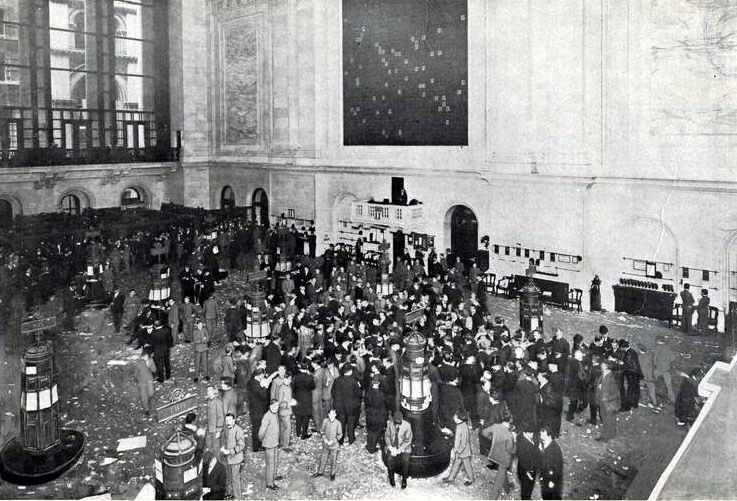
\includegraphics[height=0.34\textheight]{ch8_nyse_floor_1908.jpg}\\[1mm]
\imgcap{Bursa din New York, 1908}
\imgcredit{https://commons.wikimedia.org/wiki/File:Stockexchange.jpg}{Foto: Helen D. Van Eaton, Leslie's Monthly Magazine (1908); public domain; Wikimedia Commons}
\end{column}
\begin{column}{0.56\textwidth}
\begin{itemize}
    \item 1982--1986: ARCH și GARCH \refEng, \refBol: volatilitatea ca varianță condiționată filtrată a randamentelor zilnice
    \item 1992--2004: teoria QML \refBW, \refLH, \refLum, \refFZa; componente \refEL; DCC \refEngD
    \item 1998--2008: varianța realizată \refAB, \refABDL, \refBNSa; variația bipower \refBNSb; zgomot și kernel-uri \refZMA, \refBNHLSa
    \item 2009--2019: HAR \refCor, Realized GARCH \refHHS, GARCH-MIDAS \refEGS, HARQ \refBPQ, DCC-NL \refELW
    \item Astăzi: datele de înaltă frecvență sînt ieftine; întrebările sînt statistice (zgomot, salturi, dimensiune, evaluare)
\end{itemize}
\end{column}
\end{columns}
\end{frame}


%=============================================================================
\section{Verosimilitatea cvasi-maximă pentru GARCH}
%=============================================================================

\begin{frame}{De la TSA la acest capitol}
\itemsize{\small}
\begin{itemize}
    \item Cunoscut (\atschlink{https://danpele.github.io/Time-Series-Analysis/RO/Cursuri/capitol5_volatilitate_conditionata_garch.pdf}{TSA, Capitolul 5}): GARCH(1,1), GJR, EGARCH, curba de impact a știrilor, ML cu erori gaussiene și Student-$t$, QLIKE; (\atschlink{https://danpele.github.io/Time-Series-Analysis/RO/Cursuri/capitol14_modele_garch_multivariate.pdf}{TSA, Capitolul 14}): CCC și DCC
    \item Nou aici
    \begin{itemize}
        \item de ce ML gaussian funcționează și cînd randamentele nu sînt gaussiene și ce erori standard sînt atunci valide
        \item volatilitate cu o componentă lentă, determinată de factori macroeconomici; volatilitate măsurată din prețurile intraday, cu propria eroare de eșantionare
        \item modele care folosesc măsuri realizate; evaluarea față de o țintă zgomotoasă; matrice de covarianță cu multe active
    \end{itemize}
    \item Volatilitatea stochastică (un logaritm al varianței latent, cu propriul șoc): \atschlink{https://danpele.github.io/Advanced-Time-Series/RO/Cursuri/capitol6_modele_spatiul_starilor_filtrare_bayesiana.pdf}{Capitolul 6}; GARCH cu schimbare de regim: \atschlink{https://danpele.github.io/Advanced-Time-Series/RO/Cursuri/capitol7_modele_schimbare_regim.pdf}{Capitolul 7}; backtesting pentru VaR și ES: \atschlink{https://danpele.github.io/Advanced-Time-Series/RO/Cursuri/capitol9_var_es_backtesting.pdf}{Capitolul 9}; rough volatility: \atschlink{https://danpele.github.io/Advanced-Time-Series/RO/Cursuri/capitol10_memorie_lunga_rough_volatility.pdf}{Capitolul 10}
\end{itemize}
\end{frame}

\begin{frame}{Cvasi-verosimilitatea gaussiană (1/2): modelul}
\itemsize{\small}
\begin{itemize}
    \item Șocul randamentului este produsul dintre volatilitate și un șoc standardizat; varianța urmează recursia GARCH(1,1)
    \[ \varepsilon_t = \sigma_t(\theta_0)\,\eta_t, \qquad \sigma^2_t(\theta) = \omega + \alpha\varepsilon^2_{t-1} + \beta\sigma^2_{t-1}(\theta) \]
    \item Notațiile
    \begin{itemize}
        \item $\varepsilon_t$: randamentul centrat al zilei $t$; $\sigma^2_t(\theta)$: varianța lui condiționată de trecutul $\mathcal F_{t-1}$ (informația pînă în ziua $t-1$)
        \item $\eta_t$: șoc standardizat i.i.d., $\E\eta_t = 0$, $\E\eta_t^2 = 1$; legea lui (distribuția Normală, Student-$t$, asimetrică) este necunoscută
        \item $\theta = (\omega, \alpha, \beta)$, cu valoarea adevărată $\theta_0$: $\omega > 0$ fixează nivelul, $\alpha \ge 0$ reacția la pătratul șocului de ieri, $\beta \ge 0$ persistența varianței de ieri
    \end{itemize}
    \item Recursia pornește de la un $\sigma^2_1$ arbitrar; efectul valorii de start dispare geometric cînd $\beta < 1$
\end{itemize}
\end{frame}

\begin{frame}{Cvasi-verosimilitatea gaussiană (2/2): estimatorul și scorul}
\itemsize{\small}
\begin{itemize}
    \item QMLE: se maximizează log-verosimilitatea gaussiană, folosită ca ecuație de estimare chiar dacă $\eta_t$ nu este gaussian
    \[ \hat\theta = \arg\max_\theta \sum_{t=1}^T \ell_t(\theta), \qquad \ell_t(\theta) = -\frac12\Big(\ln\sigma^2_t(\theta) + \frac{\varepsilon_t^2}{\sigma^2_t(\theta)}\Big) \]
    \begin{itemize}
        \item $\ell_t$: log-densitatea gaussiană a zilei $t$, fără constantă; $T$: numărul de zile; $\hat\theta$: valoarea estimată
    \end{itemize}
    \item Scorul, adică gradientul lui $\ell_t$, are media condiționată zero în valoarea adevărată
    \[ s_t(\theta) = \frac{\partial\ell_t}{\partial\theta} = \frac12\Big(\frac{\varepsilon_t^2}{\sigma_t^2} - 1\Big)\frac{1}{\sigma^2_t}\frac{\partial\sigma^2_t}{\partial\theta} \]
    \begin{itemize}
        \item în $\theta_0$, $\varepsilon_t^2/\sigma_t^2 = \eta_t^2$, deci $\E(s_t | \mathcal F_{t-1}) = 0$, pentru că $\E\eta_t^2 = 1$
        \item doar varianța condiționată trebuie să fie corect specificată; forma legii lui $\eta_t$ nu se folosește niciodată
    \end{itemize}
    \item Scorul este o diferență de martingal (media condiționată de trecut este zero)
    \begin{itemize}
        \item o TLC pentru martingale dă normalitatea asimptotică fără independența lui $\varepsilon_t$
    \end{itemize}
\end{itemize}
\end{frame}

\begin{frame}{Consistența și normalitatea asimptotică (1/2): staționaritatea și consistența}
\itemsize{\small}
\begin{itemize}
    \item GARCH(1,1) este strict staționar dacă și numai dacă logaritmul multiplicatorului zilnic al varianței are media negativă
    \[ \E\ln(\alpha_0\eta_t^2 + \beta_0) < 0 \]
    \begin{itemize}
        \item $\alpha_0\eta_t^2 + \beta_0$: factorul cu care un șoc al varianței este transmis de la o zi la următoarea; $\alpha_0, \beta_0$: valorile adevărate
        \item prin inegalitatea lui Jensen, condiția este mai slabă decît $\alpha_0 + \beta_0 < 1$ (varianță finită): IGARCH ($\alpha_0 + \beta_0 = 1$) este strict staționar, iar $\E\varepsilon_t^2$ poate fi infinită
        \item \refLH, \refLum: GARCH(1,1), inclusiv IGARCH; \refBHK, \refFZa: GARCH($p,q$) sub staționaritate strictă
    \end{itemize}
    \item Consistența lui $\hat\theta$ \refFZa
    \begin{itemize}
        \item condiții: staționaritate strictă, $\theta_0$ într-o mulțime compactă de parametri, identificabilitate ($\eta_t^2$ nu este o constantă)
        \item nu este nevoie de niciun moment al lui $\varepsilon_t$
    \end{itemize}
    \item Chiar și pentru GARCH exploziv ($\E\ln(\alpha_0\eta^2 + \beta_0) > 0$), $(\hat\alpha, \hat\beta)$ rămîn consistenți și asimptotic normali, iar $\omega$ nu este identificat \refJR
\end{itemize}
\end{frame}

\begin{frame}{Consistența și normalitatea asimptotică (2/2): legea limită}
\itemsize{\small}
\begin{itemize}
    \item Dacă $\theta_0$ este interior mulțimii parametrilor și $\eta_t$ are momentul de ordinul patru finit, estimatorul este asimptotic normal
    \[ \sqrt T(\hat\theta - \theta_0) \to N\big(0, (\kappa_\eta - 1)J^{-1}\big), \qquad J = \E\Big[\frac{1}{\sigma^4_t}\frac{\partial\sigma^2_t}{\partial\theta}\frac{\partial\sigma^2_t}{\partial\theta'}\Big] \]
    \begin{itemize}
        \item $\kappa_\eta = \E\eta_t^4$: kurtosis-ul șocului ($3$ pentru distribuția Normală); $\kappa_\eta - 1 = \Var(\eta_t^2)$
        \item $J$: o matrice $3 \times 3$, media produsului exterior al sensibilităților relative $\sigma_t^{-2}\partial\sigma^2_t/\partial\theta$; $\to$: convergența în distribuție cînd $T \to \infty$
        \item interpretare: varianța de eșantionare a lui $\hat\theta$ crește liniar cu kurtosis-ul șocurilor
    \end{itemize}
    \item Frontiera: dacă $\alpha_0 = 0$, $\theta_0$ nu este interior, iar limita este proiecția unui vector normal pe un con
    \begin{itemize}
        \item de aceea \atschlink{https://danpele.github.io/Time-Series-Analysis/RO/Cursuri/capitol5_volatilitate_conditionata_garch.pdf}{TSA, Capitolul 5} testează efectele ARCH unilateral
    \end{itemize}
\end{itemize}
\end{frame}

\begin{frame}{Sandwich-ul și erorile standard Bollerslev--Wooldridge (1/2)}
\itemsize{\small}
\begin{itemize}
    \item Rezultatul general QML: varianța asimptotică este un „sandwich” format din două matrice
    \[ \sqrt T(\hat\theta - \theta_0) \to N(0, A^{-1}B\,A^{-1}), \qquad A = -\E\frac{\partial^2\ell_t}{\partial\theta\,\partial\theta'}, \qquad B = \E\,s_ts_t' \]
    \begin{itemize}
        \item $A$: hessiana negativă așteptată (curbura log-verosimilității); $B$: varianța scorului $s_t$
        \item dacă verosimilitatea este cea adevărată, $A = B$ (egalitatea informațională), iar varianța devine $A^{-1}$; sub QML, $A \ne B$
    \end{itemize}
    \item Pentru GARCH, ambele matrice sînt proporționale cu $J$ (\atsapplink{atsapp1}{atssrc1}{Anexa})
    \[ A = \tfrac12J, \qquad B = \tfrac{\kappa_\eta - 1}{4}J, \qquad A^{-1}B\,A^{-1} = (\kappa_\eta - 1)J^{-1} \]
    \begin{itemize}
        \item sandwich-ul regăsește legea limită de pe slide-ul anterior, pentru orice lege a lui $\eta_t$ cu $\kappa_\eta < \infty$
    \end{itemize}
\end{itemize}
\end{frame}

\begin{frame}{Sandwich-ul și erorile standard Bollerslev--Wooldridge (2/2)}
\itemsize{\small}
\begin{itemize}
    \item Trei moduri de a calcula erorile standard
    \begin{itemize}
        \item doar din hessiană: $A^{-1} = 2J^{-1}$, corect doar dacă $\kappa_\eta = 3$; prea mici cu factorul $\sqrt{(\kappa_\eta - 1)/2}$ cînd $\kappa_\eta > 3$
        \item din produsul exterior al scorurilor (OPG): $B^{-1} = \frac{4}{\kappa_\eta - 1}J^{-1}$, și mai mici cînd $\kappa_\eta > 3$
        \item sandwich \refBW: $\hat A^{-1}\hat B\hat A^{-1}$, valabil oricare ar fi legea lui $\eta_t$ (cu $\kappa_\eta < \infty$)
    \end{itemize}
    \item Estimațiile folosite de Bollerslev și Wooldridge
    \begin{itemize}
        \item $\hat A$: hessiana observată a lui $-\frac1T\sum_t\ell_t$ în $\hat\theta$; $\hat B = \frac1T\sum_t\hat s_t\hat s_t'$, cu $\hat s_t = s_t(\hat\theta)$ scorul estimat
    \end{itemize}
    \item Testele Wald și de tip scor robuste folosesc sandwich-ul
    \begin{itemize}
        \item statistica raportului de cvasi-verosimilitate (cvasi-LR) nu mai are distribuția $\chi^2$, ci este o sumă ponderată de variabile $\chi^2_1$ (hi-pătrat cu un grad de libertate)
    \end{itemize}
\end{itemize}
\end{frame}

\begin{frame}{Hessiana față de sandwich: un experiment Monte Carlo}
\itemsize{\footnotesize}
\begin{center}
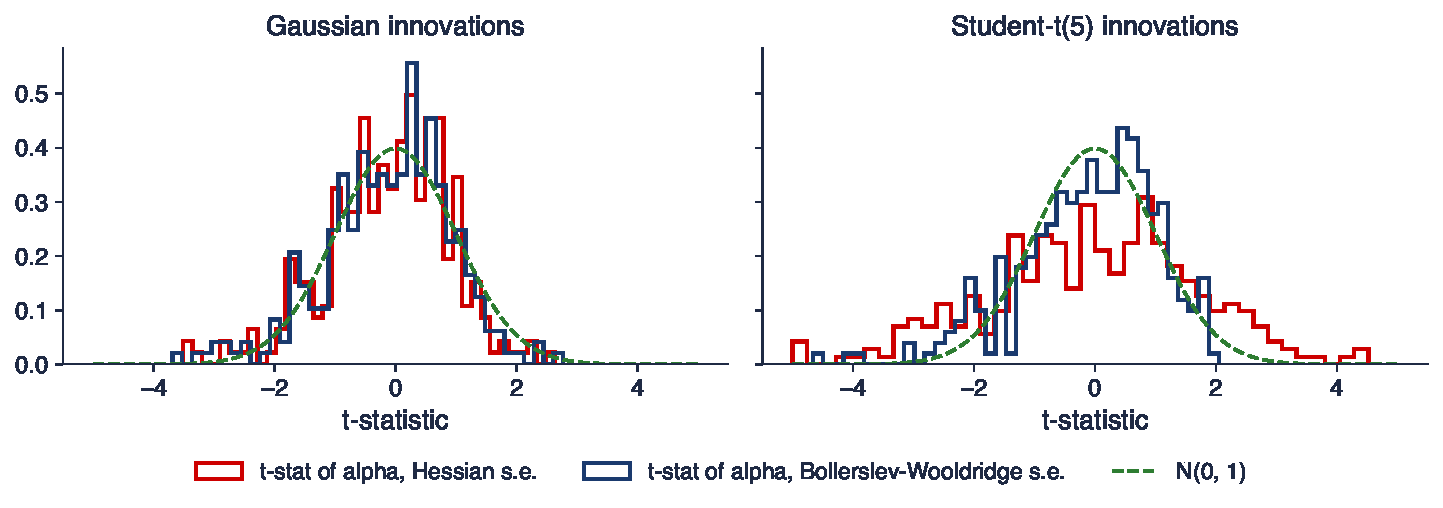
\includegraphics[width=0.97\textwidth,height=0.6\textheight,keepaspectratio]{ats_ch8_qmle_sim.pdf}
\end{center}
\vspace{-0.25cm}
\begin{itemize}
    \item GARCH(1,1) cu $(\omega, \alpha, \beta) = (0{,}05, 0{,}08, 0{,}90)$, $T = 2\,000$, 300 de replicări; QML gaussian în fiecare; histograma lui $(\hat\alpha - \alpha_0)/\widehat{\mathrm{se}}$
\end{itemize}
\quantlet{ATS\_ch8\_qmle}{\qlurl{ATS_ch8_qmle}}
\end{frame}

\begin{frame}{Interpretarea experimentului Monte Carlo}
\itemsize{\small}
\begin{itemize}
    \item $\eta$ gaussian: acoperirea intervalelor de 95\% pentru $\alpha$ este 95{,}0\% (hessiană) și 94{,}3\% (sandwich): ambele corecte
    \item Student-$t(5)$, $\kappa_\eta = 9$: intervalele din hessiană acoperă 73{,}0\% pentru $\alpha$ și 74{,}7\% pentru $\beta$; intervalele sandwich 91{,}7\% și 92{,}3\%
    \item Teoria prezice factorul $\sqrt{(9 - 1)/2} = 2$ între cele două erori standard; estimațiile punctuale sînt aceleași
    \item Cu cozi groase, un test $t$ pentru $\alpha$ construit cu erorile standard din hessiană respinge mult prea des: raportați implicit erorile standard sandwich
\end{itemize}
\end{frame}

\begin{frame}{Erori standard robuste și naive pe cinci piețe}
\itemsize{\footnotesize}
\begin{center}
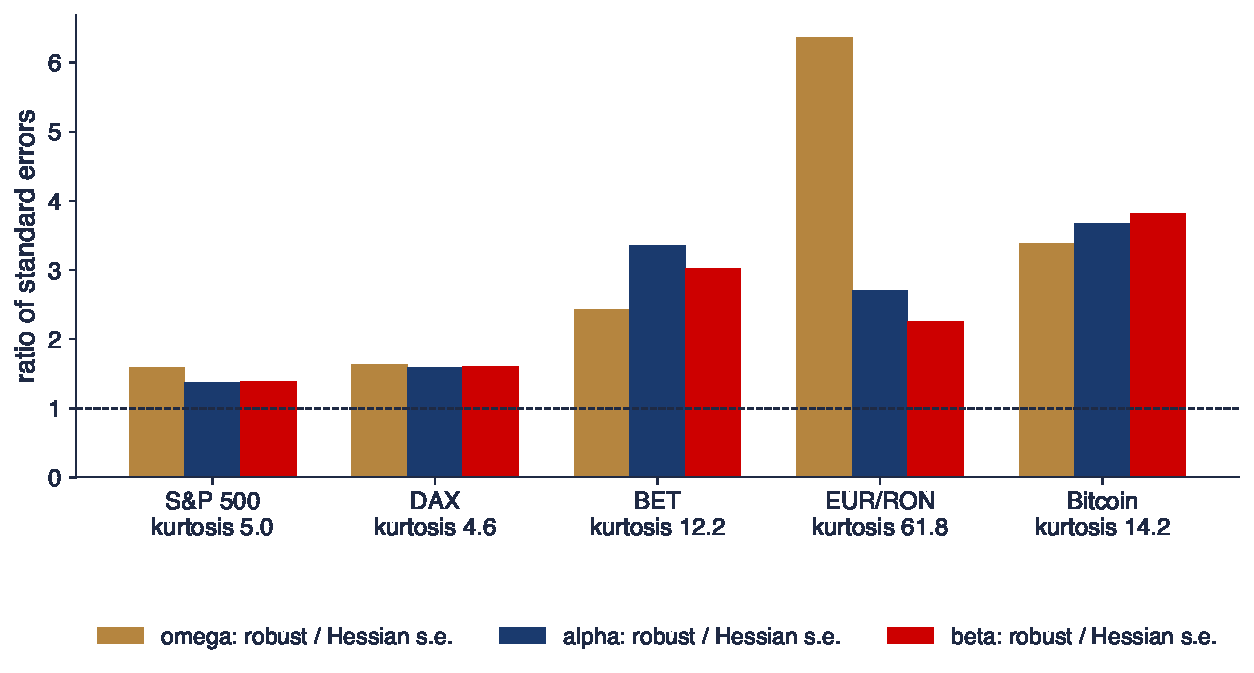
\includegraphics[width=0.97\textwidth,height=0.6\textheight,keepaspectratio]{ats_ch8_qmle_markets.pdf}
\end{center}
\vspace{-0.25cm}
\begin{itemize}
    \item QML gaussian pentru GARCH(1,1), randamente zilnice 2010--2026; bare: eroarea standard sandwich împărțită la eroarea standard din hessiană; etichete: kurtosis-ul $\hat\kappa_\eta$ al reziduurilor standardizate
\end{itemize}
\quantlet{ATS\_ch8\_qmle}{\qlurl{ATS_ch8_qmle}}
\end{frame}

\begin{frame}{Interpretarea celor cinci piețe}
\itemsize{\small}
\begin{itemize}
    \item S\&P 500: $\hat\alpha = 0{,}154$, cu eroarea standard 0{,}013 (hessiană) față de 0{,}018 (sandwich); $\hat\kappa_\eta = 5{,}0$, factorul teoretic 1{,}42
    \item BET: $\hat\kappa_\eta = 12{,}2$, eroarea standard sandwich a lui $\hat\alpha$ este de 3{,}36 ori mai mare; EUR/RON (managed float): de 2{,}71 ori, $\hat\kappa_\eta = 61{,}8$
    \item Rapoartele urmează doar aproximativ $\sqrt{(\hat\kappa_\eta - 1)/2}$: în date, $\eta_t$ nu este i.i.d., iar sandwich-ul nu are nevoie de această ipoteză
    \item ML Student-$t$ crește log-verosimilitatea cu 124{,}4 (S\&P 500) și 233{,}0 (BET), dar este consistent doar dacă forma $t$ este corectă; QML are nevoie doar de ecuația varianței
\end{itemize}
\end{frame}

\begin{frame}{Recapitulare: QML pentru GARCH}
\itemsize{\small}
\begin{itemize}
    \item QML gaussian este consistent dacă ecuația varianței este corectă, oricare ar fi forma inovațiilor
    \item Teoria are nevoie de staționaritate strictă, nu de varianță finită; IGARCH și chiar GARCH exploziv sînt acoperite
    \item Cu cozi groase, erorile standard din hessiană sînt prea mici cu factorul $\sqrt{(\kappa_\eta - 1)/2}$; folosiți Bollerslev--Wooldridge
\end{itemize}
\end{frame}


%=============================================================================
\section{Volatilitatea de termen lung și de termen scurt}
%=============================================================================

\begin{frame}{GARCH cu variabile exogene}
\itemsize{\small}
\begin{itemize}
    \item GARCH-X: valoarea de ieri a unei variabile observate intră în ecuația varianței
    \[ \sigma^2_t = \omega + \alpha\varepsilon^2_{t-1} + \beta\sigma^2_{t-1} + \pi'x_{t-1} \]
    \begin{itemize}
        \item $x_{t-1}$: vectorul variabilelor exogene cunoscute la sfîrșitul zilei $t-1$; $\pi$: coeficienții lor ($\pi'x$: suma ponderată)
        \item pozitivitatea lui $\sigma^2_t$: $x_{t-1} \ge 0$ și $\pi \ge 0$ sau o specificare în logaritmi
    \end{itemize}
    \item Candidați pentru $x_t$: o măsură realizată (duce la HEAVY și Realized GARCH, mai jos), VIX, un indice macroeconomic sau de incertitudine a politicilor, volumul tranzacțiilor
    \begin{itemize}
        \item teoria QML se păstrează dacă $x_t$ este staționar și ergodic; dinamica lui nu trebuie modelată pentru prognoze cu un pas
        \item prognozele cu mai mulți pași au nevoie de un model pentru $x_t$: exact acest lucru adaugă Realized GARCH și HEAVY
    \end{itemize}
    \item O variabilă lentă (o serie macroeconomică lunară) nu poate intra în recursia zilnică la frecvența ei: este nevoie de o structură pe componente (slide-urile următoare)
\end{itemize}
\end{frame}

\begin{frame}{Component GARCH al lui Engle și Lee (1/2): modelul}
\itemsize{\small}
\begin{itemize}
    \item \refEL: varianța este suma dintre un nivel de termen lung $q_t$, care se mișcă lent, și o abatere tranzitorie de la acest nivel
    \[ \sigma^2_t = q_t + \alpha(\varepsilon^2_{t-1} - q_{t-1}) + \beta(\sigma^2_{t-1} - q_{t-1}) \]
    \[ q_t = \omega + \rho q_{t-1} + \phi(\varepsilon^2_{t-1} - \sigma^2_{t-1}) \]
    \begin{itemize}
        \item $q_t$: componenta de termen lung (permanentă); $\rho$: persistența ei, apropiată de 1; $\omega$: termenul ei liber
        \item $\sigma^2_t - q_t$: componenta tranzitorie; $\alpha$, $\beta$: reacția și persistența ei, cu $\alpha + \beta < \rho$
        \item $\varepsilon^2_{t-1} - \sigma^2_{t-1}$: surpriza de varianță de ieri (cu media zero); $\phi$: cît din această surpriză mută nivelul de termen lung
    \end{itemize}
    \item Ambele componente sînt determinate de același șoc: modelul este un GARCH(2,2) restricționat
\end{itemize}
\end{frame}

\begin{frame}{Component GARCH al lui Engle și Lee (2/2): două viteze}
\itemsize{\small}
\begin{itemize}
    \item Timpul de înjumătățire: numărul de zile după care jumătate dintr-un șoc al unei componente a dispărut
    \[ \mathrm{HL}_q = \frac{\ln(1/2)}{\ln\rho}, \qquad \mathrm{HL}_{\sigma - q} = \frac{\ln(1/2)}{\ln(\alpha + \beta)} \]
    \begin{itemize}
        \item $\mathrm{HL}_q$: timpul de înjumătățire al componentei de termen lung; $\mathrm{HL}_{\sigma - q}$: al componentei tranzitorii
        \item o persistență $\rho = 0{,}99$ dă aproximativ 69 de zile; $\alpha + \beta = 0{,}9$ dă aproximativ 6,6 zile
        \item GARCH(1,1) impune un singur timp de înjumătățire, $\ln 0{,}5/\ln(\alpha + \beta)$
    \end{itemize}
    \item Două exponențiale aproximează, pe un interval finit de laguri, o autocorelație a pătratelor randamentelor care scade lent (hiperbolic)
    \begin{itemize}
        \item memoria lungă propriu-zisă: \atschlink{https://danpele.github.io/Advanced-Time-Series/RO/Cursuri/capitol10_memorie_lunga_rough_volatility.pdf}{Capitolul 10}
    \end{itemize}
\end{itemize}
\end{frame}

\begin{frame}{Component GARCH pentru S\&P 500}
\itemsize{\footnotesize}
\begin{center}
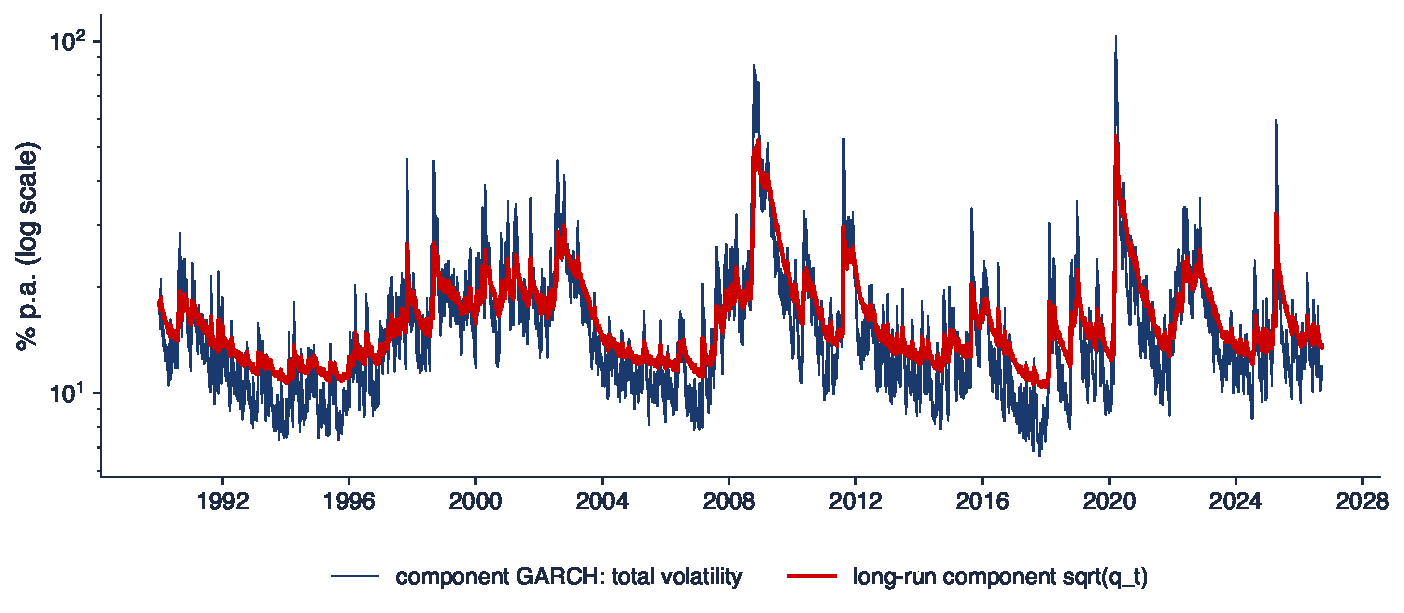
\includegraphics[width=0.97\textwidth,height=0.6\textheight,keepaspectratio]{ats_ch8_cgarch.pdf}
\end{center}
\vspace{-0.25cm}
\begin{itemize}
    \item Randamente zilnice din 1990, $T = 9\,240$; QML gaussian; volatilitatea totală anualizată $\sqrt{252\sigma^2_t}$ și componenta de termen lung $\sqrt{252q_t}$
\end{itemize}
\quantlet{ATS\_ch8\_components}{\qlurl{ATS_ch8_components}}
\end{frame}

\begin{frame}{Interpretarea modelului cu componente}
\itemsize{\small}
\begin{itemize}
    \item $\hat\rho = 0{,}995$, $\hat\phi = 0{,}026$; partea tranzitorie $\hat\alpha + \hat\beta = 0{,}950$: timpi de înjumătățire de 150 de zile (termen lung) și 13{,}6 zile (termen scurt)
    \item GARCH(1,1) pe aceleași date: persistența 0{,}983, un singur timp de înjumătățire de 41 de zile, un compromis între cele două
    \item Statistica cvasi-LR față de GARCH(1,1): 44{,}1; sub ipoteza nulă $\phi = 0$ parametrul $\rho$ nu este identificat (problema Davies), deci referința $\chi^2_2$ este doar orientativă
    \item După 2008, 2020 și 2025, nivelul de termen lung rămîne ridicat luni de zile, deși volatilitatea zilnică a scăzut deja: acest lucru contează pentru orizonturi de peste cîteva săptămîni
\end{itemize}
\end{frame}

\begin{frame}{GARCH-MIDAS (1/3): o componentă de termen lung determinată macroeconomic}
\itemsize{\footnotesize}
\begin{columns}[T]
\begin{column}{0.3\textwidth}
\centering

\includegraphics[height=0.26\textheight]{ch8_ghysels_2019.jpg}\\[1mm]
\imgcap{Eric Ghysels, 2019}
\imgcredit{https://commons.wikimedia.org/wiki/File:EricGhysels.jpg}{Foto: Eghysels (2019); CC BY-SA 4.0; Wikimedia Commons}
\end{column}
\begin{column}{0.68\textwidth}
\begin{itemize}
    \item \refEGS: varianța zilnică este produsul dintre un nivel lunar $\tau_t$ și un factor zilnic $g_{i,t}$
    \[ r_{i,t} = \mu + \sqrt{\tau_t\,g_{i,t}}\;\eta_{i,t} \]
    \begin{itemize}
        \item $r_{i,t}$: randamentul zilei $i$ din luna $t$; $\mu$: randamentul mediu; $\eta_{i,t}$: șoc i.i.d. cu media 0 și varianța 1
    \end{itemize}
    \item Termenul scurt: un GARCH(1,1) cu media 1, rescalat cu $\tau_t$
    \[ g_{i,t} = (1 - \alpha - \beta) + \alpha\frac{(r_{i-1,t} - \mu)^2}{\tau_t} + \beta g_{i-1,t} \]
    \begin{itemize}
        \item $\alpha$, $\beta$: reacția și persistența componentei zilnice, ca în GARCH(1,1)
    \end{itemize}
\end{itemize}
\end{column}
\end{columns}
\end{frame}

\begin{frame}{GARCH-MIDAS (2/3): componenta de termen lung}
\itemsize{\small}
\begin{itemize}
    \item Termenul lung: o regresie MIDAS (mixed-data sampling, eșantionare cu frecvențe mixte) a lui $\ln\tau_t$ pe $K$ laguri ale unei variabile lunare
    \[ \ln\tau_t = m + \theta\sum_{k=1}^K\varphi_k(w)\,X_{t-k}, \qquad \varphi_k(w) \propto (1 - k/K)^{w - 1} \]
    \begin{itemize}
        \item $X_{t-k}$: factorul lunar de acum $k$ luni; $m$: termenul liber; $\theta$: efectul factorului (semnul arată dacă este prociclic sau anticiclic)
        \item $\varphi_k(w)$: ponderi beta pe laguri, normalizate să însumeze 1 și restricționate să scadă \refGSV; $w \ge 1$: cu cît $w$ este mai mare, cu atît scad mai repede; $w = 1$: ponderi egale
    \end{itemize}
    \item Alegeri pentru $X$
    \begin{itemize}
        \item varianța realizată din lunile anterioare, în nivel: $\tau_t = m + \theta\sum_k\varphi_k(w)\mathrm{RV}_{t-k}$, cu $\mathrm{RV}_{t-k}$ suma pătratelor randamentelor zilnice din luna $t-k$
        \item date macroeconomice: creșterea producției industriale, inflația IPP
    \end{itemize}
\end{itemize}
\end{frame}

\begin{frame}{GARCH-MIDAS (3/3): identificare, estimare și raportul de varianță}
\itemsize{\small}
\begin{itemize}
    \item $\tau_t$ este constant în cadrul lunii, iar $\E g_{i,t} = 1$: descompunerea este identificată prin frecvențele diferite, fără un filtru pentru o variabilă latentă
    \begin{itemize}
        \item QML gaussian pentru toți parametrii $(\mu, \alpha, \beta, m, \theta, w)$ într-un singur pas; erori standard sandwich
    \end{itemize}
    \item Raportul de varianță: ponderea variației logaritmului volatilității explicată de componenta de termen lung
    \[ \mathrm{VR} = \frac{\Var(\ln\tau_t)}{\Var(\ln(\tau_t\,g_{i,t}))} \in [0, 1] \]
    \begin{itemize}
        \item VR apropiat de 0: componenta de termen lung este aproape constantă; apropiat de 1: ea preia cea mai mare parte a variației
        \item o variabilă macroeconomică poate fi semnificativă ($\hat\theta \ne 0$) și totuși să explice puțin din volatilitatea zilnică (VR mic)
    \end{itemize}
    \item Inferența asupra lui $w$ este nestandard cînd $\theta = 0$ ($w$ nu este atunci identificat) și la frontiera $w = 1$
    \item Extensii: ponderi nerestricționate, mai mulți regresori, o a doua componentă (zilnică) \refCK; prognozele de peste o lună folosesc doar partea de termen lung
\end{itemize}
\end{frame}

\begin{frame}{Studiu de caz: Engle, Ghysels și Sohn (2013) pe datele noastre}
\itemsize{\small}
\begin{itemize}
    \item \textbf{Întrebarea} din \refEGS: se mișcă volatilitatea de termen lung a pieței de acțiuni împreună cu fundamentele macroeconomice (creșterea producției, inflația)?
    \begin{itemize}
        \item eșantionul lor de randamente ale acțiunilor din SUA este mult mai lung decît al nostru; componenta lor de termen lung de referință este o varianță realizată pe ferestre fixe
    \end{itemize}
    \item \textbf{Replicarea noastră}: randamentele zilnice ale S\&P 500, eșantion comun din 04.01.1993, $T = 8\,482$; $K = 36$ laguri lunare; ponderi beta restricționate
    \begin{itemize}
        \item trei factori de termen lung: varianța realizată lunară (suma pătratelor randamentelor zilnice), creșterea producției industriale (FRED INDPRO), inflația IPP (FRED WPSFD49207)
        \item toate modelele comparate cu GARCH(1,1) pe aceleași zile; QML cu erori standard sandwich
    \end{itemize}
    \item Extindere pentru un proiect: producția industrială a României și BET (Seminarul 8, B5); edițiile în timp real ale datelor macroeconomice
\end{itemize}
\end{frame}

\begin{frame}{GARCH-MIDAS pentru S\&P 500}
\itemsize{\footnotesize}
\begin{center}
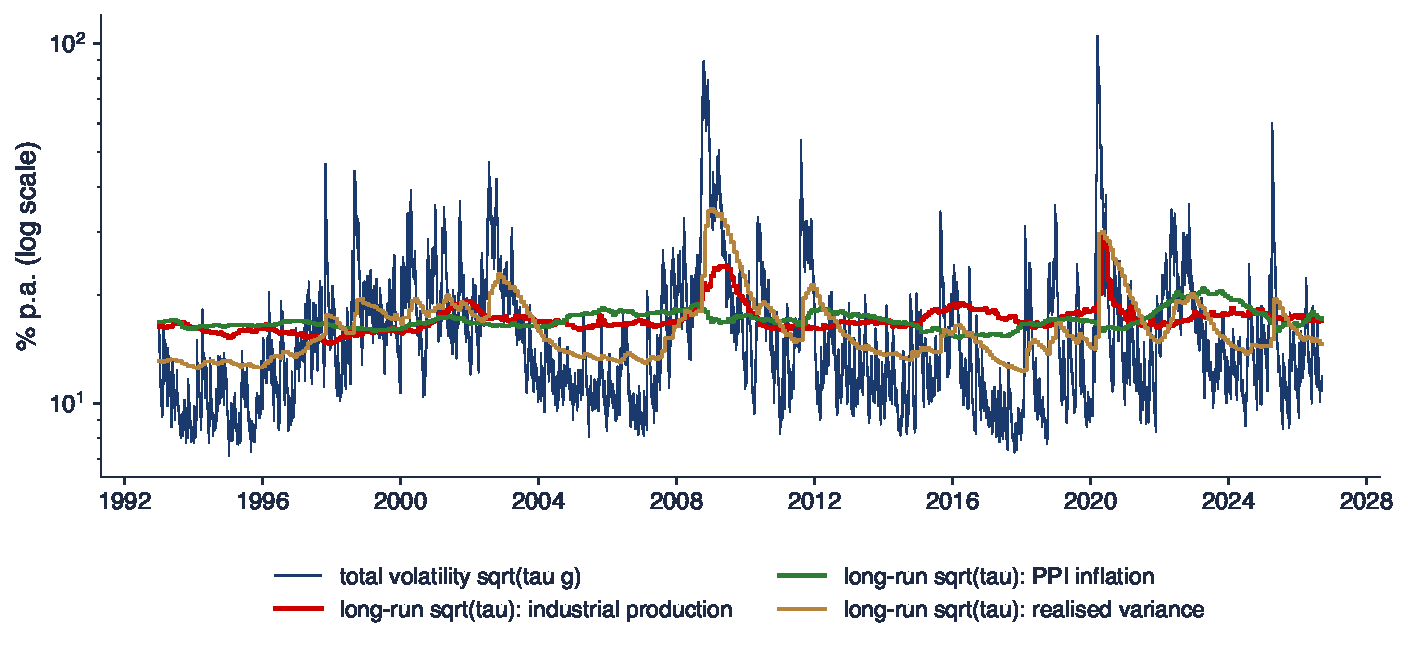
\includegraphics[width=0.97\textwidth,height=0.6\textheight,keepaspectratio]{ats_ch8_garch_midas.pdf}
\end{center}
\vspace{-0.25cm}
\begin{itemize}
    \item $\sqrt{252\tau_tg_{i,t}}$ anualizat pentru modelul cu producția industrială și componentele de termen lung $\sqrt{252\tau_t}$ ale celor trei modele
\end{itemize}
\quantlet{ATS\_ch8\_components}{\qlurl{ATS_ch8_components}}
\end{frame}

\begin{frame}{Estimațiile GARCH-MIDAS}
\itemsize{\small}
\begin{center}
\scriptsize
\begin{tabular}{lcccccc}
\toprule
\textbf{Factorul de termen lung} & $\hat\alpha$ & $\hat\beta$ & $\hat\theta$ (s.e.) & $\hat w$ & VR (\%) & BIC \\
\midrule
varianța realizată (nivel) & 0{,}119 & 0{,}841 & 0{,}0225 (0{,}0058) & 5{,}939 & 25{,}1 & 22710{,}0 \\
creșterea producției industriale & 0{,}110 & 0{,}870 & \ensuremath{-}0{,}551 (0{,}353) & 3{,}692 & 4{,}5 & 22732{,}5 \\
inflația IPP & 0{,}108 & 0{,}873 & 0{,}753 (1{,}260) & 1{,}000 & 2{,}2 & 22733{,}3 \\
GARCH(1,1) & & & & & & 22721{,}9 \\
\bottomrule
\end{tabular}
\end{center}
\begin{itemize}
    \item Aceleași zile pentru toate modelele; BIC $= -2\ln L + k\ln T$ (mai mic este mai bine); erori standard: Bollerslev--Wooldridge
\end{itemize}
\end{frame}

\begin{frame}{Interpretarea modelului GARCH-MIDAS}
\itemsize{\small}
\begin{itemize}
    \item Varianța realizată ca factor lent: $\hat\theta = 0{,}0225$ ($t = 3{,}86$), VR = 25{,}1\%, BIC sub GARCH(1,1): o componentă de termen lung există
    \item Producția industrială: $\hat\theta = \ensuremath{-}0{,}551$ ($t = \ensuremath{-}1{,}56$), semnul anticiclic din \refEGS, dar VR doar 4{,}5\% și un BIC mai mare decît GARCH(1,1)
    \item Inflația IPP: $\hat w$ la frontiera 1 (ponderi egale) și $\hat\theta$ imprecis: nicio dovadă în 1993--2026
    \item Verdictul replicării: semnul calitativ se păstrează, intensitatea nu; efectele macroeconomice au nevoie de eșantioane lungi, cu recesiuni adînci, motiv pentru care studiul original folosește o istorie mult mai lungă
\end{itemize}
\end{frame}

\begin{frame}{Recapitulare: componentele de termen lung}
\itemsize{\small}
\begin{itemize}
    \item Volatilitatea are cel puțin două viteze; o singură persistență GARCH le face media
    \item GARCH-MIDAS permite unei variabile lunare să determine nivelul de termen lung; identificarea vine din frecvențele mixte
    \item Raportați VR și BIC alături de $\hat\theta$: semnificația statistică nu înseamnă importanță
\end{itemize}
\end{frame}


%=============================================================================
\section{Măsuri realizate: teorie, zgomot și kernel-uri}
%=============================================================================

\begin{frame}{Prețurile ca semimartingale Itô (1/2): modelul}
\itemsize{\small}
\begin{itemize}
    \item În cursul zilei $t$, logaritmul prețului se modifică printr-un drift, o componentă browniană scalată cu volatilitatea instantanee și salturi
    \[ dX_s = \mu_s\,ds + \sigma_s\,dW_s + dJ_s, \qquad s \in [0, 1] \]
    \begin{itemize}
        \item $X_s$: logaritmul prețului la momentul intraday $s$ (ziua este rescalată la $[0, 1]$); $\mu_s$: drift-ul; $W_s$: mișcarea browniană standard
        \item $\sigma_s$: volatilitatea instantanee (spot), stochastică; $J_s$: un proces de salturi cu un număr finit de salturi pe zi, $\Delta J_s$: saltul din momentul $s$
    \end{itemize}
    \item Variația pătratică a zilei: partea de difuzie plus pătratele salturilor
    \[ \mathrm{QV}_t = \mathrm{IV}_t + \sum_{s \le 1}(\Delta J_s)^2, \qquad \mathrm{IV}_t = \int_0^1\sigma^2_s\,ds \]
    \begin{itemize}
        \item $\mathrm{IV}_t$: varianța integrată, media varianței instantanee pe parcursul zilei
        \item fără salturi și cu $\sigma$ independent de $W$: $r_t | \mathrm{IV}_t \sim N(\int_0^1\mu_s\,ds, \mathrm{IV}_t)$, deci IV este varianța relevantă pentru randamentul zilnic $r_t$
    \end{itemize}
\end{itemize}
\end{frame}

\begin{frame}{Prețurile ca semimartingale Itô (2/2): varianța realizată}
\itemsize{\small}
\begin{itemize}
    \item Varianța realizată: suma pătratelor celor $n$ randamente intraday ale zilei
    \[ \mathrm{RV}_t = \sum_{i=1}^n r_{t,i}^2, \qquad r_{t,i} = X_{i/n} - X_{(i-1)/n} \]
    \begin{itemize}
        \item $n$: numărul intervalelor intraday (78 de randamente la 5 minute într-o ședință de 6,5 ore); $r_{t,i}$: randamentul logaritmic din intervalul $i$
        \item $\mathrm{RV}_t \to \mathrm{QV}_t$ în probabilitate cînd $n \to \infty$: RV măsoară variația totală (difuzie plus salturi)
    \end{itemize}
    \item Drift-ul nu contează la limită: este $O(1/n)$ pe interval, în timp ce partea browniană este $O(n^{-1/2})$
    \begin{itemize}
        \item volatilitatea devine observabilă \emph{ex post}, fără model \refABDL, \refBNSa
    \end{itemize}
\end{itemize}
\end{frame}

\begin{frame}{Teorema limită centrală pentru varianța realizată (1/2)}
\itemsize{\small}
\begin{itemize}
    \item \refBNSa: fără salturi, eroarea lui RV scade cu rata $\sqrt n$ și este mixt normală
    \[ \sqrt n\,(\mathrm{RV}_t - \mathrm{IV}_t) \to MN(0, 2\,\mathrm{IQ}_t), \qquad \mathrm{IQ}_t = \int_0^1\sigma^4_s\,ds \]
    \begin{itemize}
        \item $\mathrm{IQ}_t$: cuarticitatea integrată, media zilnică a lui $\sigma^4_s$; ea stabilește mărimea erorii
        \item $MN$ (mixt normală): normală condiționat de traiectoria lui $\sigma$, cu o varianță aleatoare $2\,\mathrm{IQ}_t$
        \item convergența este \emph{stabilă} în lege: putem împărți la $\sqrt{\mathrm{IQ}_t}$, aleator și estimat consistent, fără a schimba limita
    \end{itemize}
    \item Rata $\sqrt n$: cu $n = 78$ și volatilitate constantă în cursul zilei, eroarea relativă este de aproximativ $\sqrt{2/78} \approx 16\%$
    \begin{itemize}
        \item eroarea de măsurare $\mathrm{RV}_t - \mathrm{IV}_t$ este heteroscedastică (crește cu $\mathrm{IQ}_t$): pe acest fapt se bazează HARQ, mai jos
    \end{itemize}
\end{itemize}
\end{frame}

\begin{frame}{Teorema limită centrală pentru varianța realizată (2/2): intervale fezabile}
\itemsize{\small}
\begin{itemize}
    \item Varianta fezabilă: estimăm IQ prin cuarticitatea realizată RQ, apoi studentizăm
    \[ \widehat{\mathrm{IQ}}_t = \mathrm{RQ}_t = \frac n3\sum_{i=1}^n r_{t,i}^4, \qquad \frac{\mathrm{RV}_t - \mathrm{IV}_t}{\sqrt{\frac23\sum_i r_{t,i}^4}} \to N(0, 1) \]
    \begin{itemize}
        \item factorul $\frac n3$ face RQ nedeplasat la volatilitate constantă, deoarece $\E Z^4 = 3$ pentru $Z \sim N(0, 1)$
        \item interval de 95\% pentru $\mathrm{IV}_t$: $\mathrm{RV}_t \pm 1{,}96\sqrt{\frac23\sum_i r_{t,i}^4}$; poate conține valori negative
    \end{itemize}
    \item Versiunea în logaritmi (metoda delta): un interval pentru $\ln\mathrm{IV}_t$
    \[ \ln\mathrm{RV}_t \pm 1{,}96\,\frac{\sqrt{\frac23\sum_i r_{t,i}^4}}{\mathrm{RV}_t} \]
    \begin{itemize}
        \item după exponențiere nu conține niciodată valori negative și are o acoperire mai bună în eșantioane finite
    \end{itemize}
\end{itemize}
\end{frame}

\begin{frame}{O piață simulată cu adevărul cunoscut}
\itemsize{\small}
\begin{itemize}
    \item Grilă la o secundă, $n = 23\,400$ de secunde pe zi; logaritmul varianței instantanee este suma a doi factori AR(1) gaussieni
    \[ \ln\sigma^2_s = c + f^{(1)}_s + f^{(2)}_s \]
    \begin{itemize}
        \item $c$: constanta care fixează media; $f^{(1)}$: factorul lent (timp de înjumătățire de 60 de zile, abaterea standard staționară 0,75); $f^{(2)}$: factorul rapid (2 zile, abaterea standard 0,45)
        \item media IV = 1 (\%$^2$ pe zi), media realised kernel-ului pentru S\&P 500 în 2000--2022; efectul de levier: corelația $-0{,}6$ între șocurile prețului și șocurile factorului rapid
    \end{itemize}
    \item Salturi: proces Poisson cu 0,08 salturi pe zi, mărimi $N(0, 0{,}8^2)$ (\%): salturile reprezintă aproximativ 5{,}6\% din variația pătratică
    \item Zgomot: observăm $Y_s = X_s + u_s$, cu $u_s$ i.i.d. $N(0, \omega^2)$ și $\omega = 0{,}004\%$
    \begin{itemize}
        \item $Y_s$: logaritmul prețului observat; $X_s$: logaritmul prețului eficient; $u_s$: zgomotul de microstructură, cu abaterea standard $\omega$; la o secundă, $2n\omega^2 = 0{,}75$ (slide-urile următoare)
    \end{itemize}
    \item Fiecare estimator de mai jos este comparat cu IV sau QV adevărate din aceeași zi simulată
\end{itemize}
\end{frame}

\begin{frame}{Acoperirea TLC fezabile}
\itemsize{\footnotesize}
\begin{center}
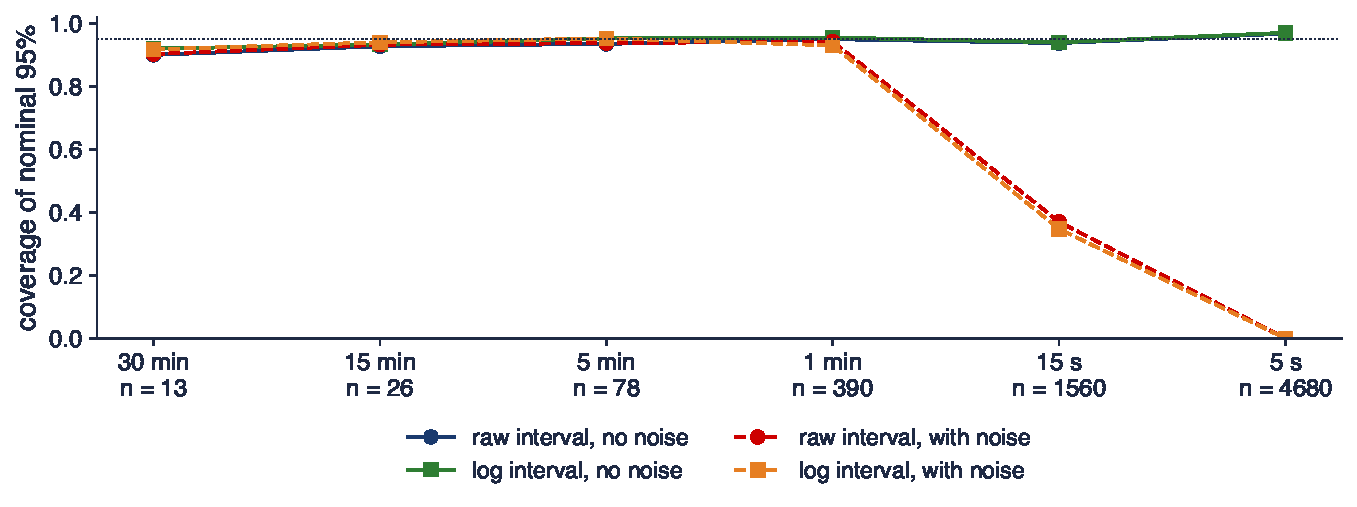
\includegraphics[width=0.97\textwidth,height=0.6\textheight,keepaspectratio]{ats_ch8_rv_clt.pdf}
\end{center}
\vspace{-0.25cm}
\begin{itemize}
    \item 400 de zile simulate fără salturi; intervale de 95\% pentru $\mathrm{IV}_t$ (în nivel și în logaritmi) din randamente eșantionate la 30 de minute pînă la 5 secunde, fără și cu zgomot
\end{itemize}
\quantlet{ATS\_ch8\_realised\_measures}{\qlurl{ATS_ch8_realised_measures}}
\end{frame}

\begin{frame}{Interpretarea acoperirii TLC}
\itemsize{\small}
\begin{itemize}
    \item Fără zgomot, acoperirea se apropie de 95\% cînd $n$ crește: intervalul în nivel are 90{,}0\% la $n = 13$ și 95{,}0\% la $n = 390$; intervalul în logaritmi este mai aproape pentru $n$ mic (92{,}0\%)
    \item Cu zgomot, acoperirea se prăbușește cînd eșantionarea este prea fină: 37{,}0\% la 15 secunde și 0{,}0\% la 5 secunde; la un minut este încă 94{,}2\%
    \item Intervalul se îngustează ca $n^{-1/2}$, iar deplasarea din zgomot crește ca $n$: TLC este o afirmație despre prețul eficient, nu despre cel observat
    \item Regula practică: randamente la 5 minute pentru active lichide, cu excepția cazului în care se folosește un estimator robust la zgomot
\end{itemize}
\end{frame}

\begin{frame}{Sursa măsurilor realizate}
\itemsize{\footnotesize}
\begin{columns}[T]
\begin{column}{0.36\textwidth}
\centering

\includegraphics[height=0.34\textheight]{ch8_barndorff_nielsen_2007.jpg}\\[1mm]
\imgcap{Ole E. Barndorff-Nielsen, 2007}
\imgcredit{https://commons.wikimedia.org/wiki/File:Ole-Barndorff-Nielsen.jpg}{Foto: Thomas Steiner (2007); CC BY-SA 2.5; Wikimedia Commons}
\end{column}
\begin{column}{0.62\textwidth}
\begin{itemize}
    \item \refOMI, versiunea 0.3: RV, BV, realised kernels și randamente deschidere--închidere zilnice pentru 31 de indici, din 2000 pînă la 25 februarie 2022, construite din date tick curățate
    \item condițiile ei: utilizare liberă dacă biblioteca și versiunea ei sînt citate; copia arhivată păstrează fișierul din 2022 disponibil după închidere
    \item Bitcoin și Ether se tranzacționează 24/7, iar Binance publică toate prețurile la un minut și la o secundă: calculăm RV, BV, RQ, cuarticitatea tripower și un realised kernel pentru fiecare zi UTC, 2018--2026
    \item Nicio sursă gratuită nu acoperă datele intraday pentru acțiuni după 2022: un proiect le poate reconstrui dintr-o sursă cu licență
\end{itemize}
\end{column}
\end{columns}
\end{frame}

\begin{frame}{Volatilitatea realizată pe mai multe piețe}
\itemsize{\footnotesize}
\begin{center}
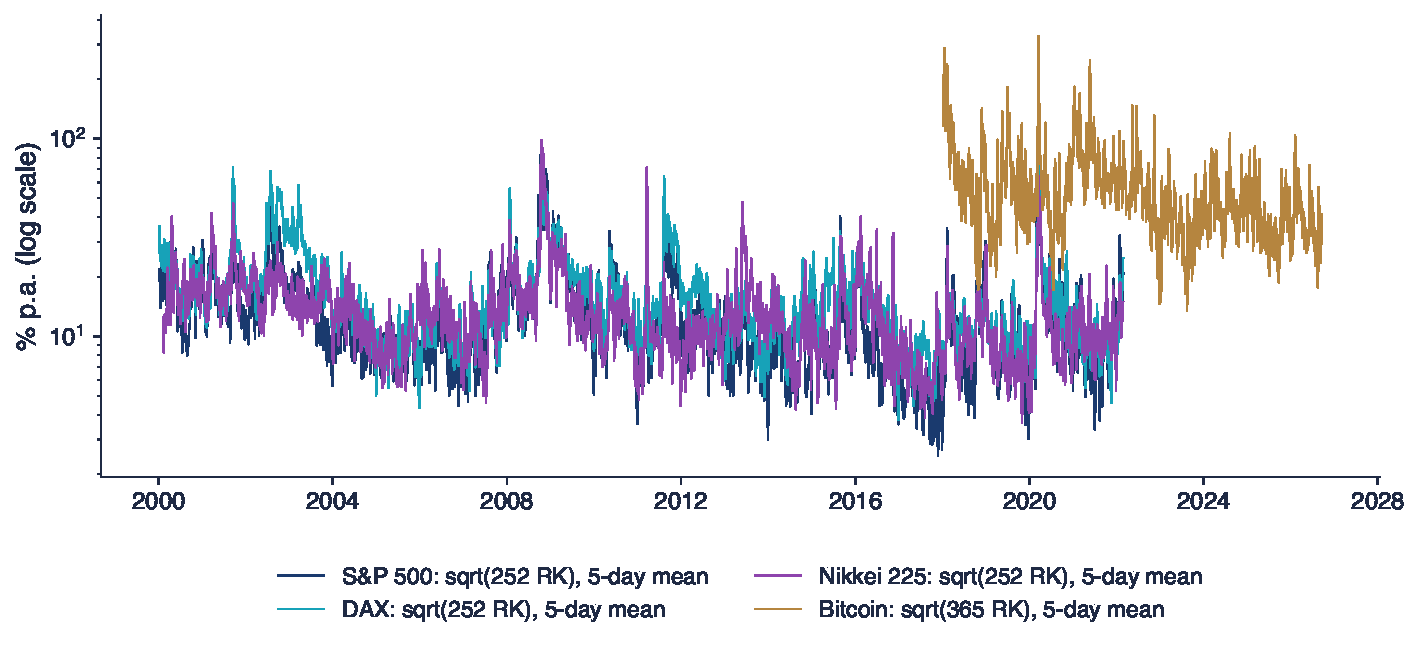
\includegraphics[width=0.97\textwidth,height=0.6\textheight,keepaspectratio]{ats_ch8_rk_overview.pdf}
\end{center}
\vspace{-0.25cm}
\begin{itemize}
    \item Realised kernel anualizat, medii pe 5 zile: S\&P 500, DAX și Nikkei 225 (Oxford-Man, 2000--2022); Bitcoin (prețuri Binance la un minut, 2018--2026, 365 de zile pe an)
\end{itemize}
\quantlet{ATS\_ch8\_realised\_measures}{\qlurl{ATS_ch8_realised_measures}}
\end{frame}

\begin{frame}{Interpretarea volatilităților realizate}
\itemsize{\small}
\begin{itemize}
    \item Volatilitatea anualizată medie din kernel: S\&P 500 16{,}2\%, DAX 19{,}5\%, Nikkei 16{,}6\%, Bitcoin 68{,}4\%
    \item Seriile de acțiuni se mișcă împreună (2002, 2008, 2011, 2020): un factor comun de termen lung, tema multivariată din ultima secțiune
    \item Măsurile deschidere--închidere omit randamentul de peste noapte: pentru riscul zilnic se adaugă pătratul randamentului de peste noapte sau se scalează măsura
    \item Bitcoin nu are perioade fără tranzacționare, dar volatilitatea lui zilnică este de trei pînă la patru ori mai mare și scade după 2023
\end{itemize}
\end{frame}

\begin{frame}{Zgomotul de microstructură (1/2): deplasarea lui RV}
\itemsize{\small}
\begin{itemize}
    \item Logaritmul prețului observat este prețul eficient plus un termen de zgomot
    \[ Y_{i/n} = X_{i/n} + u_i \]
    \begin{itemize}
        \item $u_i$: zgomot i.i.d. cu varianța $\omega^2$, independent de $X$; surse: oscilația între bid și ask, discretizarea prețului, cotațiile stale (neactualizate)
    \end{itemize}
    \item RV calculat din prețurile observate la $n$ intervale, $\mathrm{RV}^{(n)}_t$, este deplasat în sus, iar deplasarea crește cu $n$ (\atsapplink{atsapp2}{atssrc2}{Anexa})
    \[ \E(\mathrm{RV}^{(n)}_t | X) = \mathrm{IV}_t + 2n\omega^2, \qquad \Var(\mathrm{RV}^{(n)}_t | X) \approx 4n\,\E u^4 \]
    \begin{itemize}
        \item fiecare randament observat conține $u_i - u_{i-1}$, cu varianța $2\omega^2$; însumat pe $n$ randamente, aceasta dă $2n\omega^2$
        \item RV diverge cînd $n \to \infty$: eșantionarea cît mai deasă nu este optimă
    \end{itemize}
\end{itemize}
\end{frame}

\begin{frame}{Zgomotul de microstructură (2/2): diagnostice}
\itemsize{\small}
\begin{itemize}
    \item Două consecințe ale zgomotului i.i.d.
    \begin{itemize}
        \item $\hat\omega^2 = \mathrm{RV}^{(n)}_t/(2n)$, la frecvența cea mai mare, estimează varianța zgomotului, deoarece acolo $2n\omega^2$ domină IV
        \item randamentele prețului observat au autocovarianța de ordinul întîi $-\omega^2$: autocorelația negativă este amprenta zgomotului i.i.d.
    \end{itemize}
    \item Signature plot: media $\mathrm{RV}^{(n)}$ în funcție de intervalul de eșantionare
    \begin{itemize}
        \item o zonă plată arată intervalele la care zgomotul nu mai contează
    \end{itemize}
    \item Zgomotul real nu este i.i.d.: este autocorelat și corelat cu prețul eficient, mai ales în datele de cotații \refHLc
\end{itemize}
\end{frame}

\begin{frame}{Eșantionarea rară optimă}
\itemsize{\small}
\begin{itemize}
    \item Eroarea pătratică medie (MSE) a lui $\mathrm{RV}^{(n)}$ ca estimator al lui IV: varianța de eșantionare scade, deplasarea din zgomot crește cu $n$
    \[ \mathrm{MSE}(n) \approx \underbrace{\frac{2\,\mathrm{IQ}}{n}}_{\text{varianța}} + \underbrace{(2n\omega^2)^2}_{\text{deplasarea}^2} + 4n\,\E u^4 + \dots \]
    \item Minimizarea primilor doi termeni dă numărul optim de intervale \refBR
    \[ n^* \approx \Big(\frac{\mathrm{IQ}}{4\omega^4}\Big)^{1/3} \]
    \begin{itemize}
        \item grila optimă este mai rară cînd zgomotul ($\omega^2$) este mare față de volatilitate ($\mathrm{IQ}$)
        \item exemplu (Seminarul 8, A3): IV = IQ = 1, $\omega^2 = 1{,}6\times10^{-5}$ dă $n^* \approx 990$, un randament la fiecare 24 de secunde
    \end{itemize}
    \item Cel mai bun RV rar converge doar cu rata $n^{1/6}$ și renunță la majoritatea datelor: de aici estimatorii care folosesc toate observațiile
    \item Subeșantionarea: media RV pe cele $K$ grile decalate (cu start în secunda $0, 1, \dots, K-1$); aceeași deplasare, varianță mai mică
\end{itemize}
\end{frame}

\begin{frame}{Două scale de timp și realised kernels (1/2)}
\itemsize{\small}
\begin{itemize}
    \item RV cu două scale \refZMA: scala rapidă estimează deplasarea din zgomot a celei lente și o elimină
    \[ \mathrm{TSRV} = \overline{\mathrm{RV}}^{(K)} - \frac{\bar n}{n}\,\mathrm{RV}^{(n)}, \qquad \bar n = \frac{n - K + 1}{K} \]
    \begin{itemize}
        \item $\overline{\mathrm{RV}}^{(K)}$: RV subeșantionat pe $K$ grile rare decalate (scala lentă), fiecare cu aproximativ $\bar n$ randamente; $\mathrm{RV}^{(n)}$: RV pe toate cele $n$ randamente (scala rapidă)
        \item deplasarea scalei lente este $2\bar n\omega^2 = \frac{\bar n}{n}\cdot 2n\omega^2$: corecția o scade; rata $n^{1/6}$
    \end{itemize}
    \item Pre-averaging \refJLMPV: mediem randamentele pe blocuri înainte de ridicarea la pătrat
    \begin{itemize}
        \item rata $n^{1/4}$, cea optimă în prezența zgomotului; în practică, apropiat de realised kernel
    \end{itemize}
\end{itemize}
\end{frame}

\begin{frame}{Două scale de timp și realised kernels (2/2): realised kernel-ul}
\itemsize{\small}
\begin{itemize}
    \item Realised kernel \refBNHLSa: RV plus autocovarianțele realizate, ponderate
    \[ \mathrm{RK}_t = \gamma_0 + \sum_{h=1}^H k\Big(\frac{h}{H+1}\Big)(\gamma_h + \gamma_{-h}), \qquad \gamma_h = \sum_i r_{t,i}\,r_{t,i-h} \]
    \begin{itemize}
        \item $\gamma_h$: autocovarianța realizată la lagul $h$ ($\gamma_0 = \mathrm{RV}$); $H$: lățimea de bandă, numărul de laguri folosite; $k(\cdot)$: funcția de ponderare, cu $k(0) = 1$, $k(1) = 0$
        \item ponderile Parzen: $k(x) = 1 - 6x^2 + 6x^3$ pentru $x \le \frac12$ și $2(1-x)^3$ pentru $\frac12 < x \le 1$
        \item $\gamma_1$ negativ creat de zgomot anulează deplasarea $2n\omega^2$: aceeași idee ca la estimarea HAC a varianței (\atschlink{https://danpele.github.io/Advanced-Time-Series/RO/Cursuri/capitol0_recapitulare_inferenta.pdf}{Capitolul 0})
    \end{itemize}
    \item Proprietăți
    \begin{itemize}
        \item nenegativ prin construcție; rata $n^{1/5}$ cu $H = c^*\xi^{4/5}n^{3/5}$, unde $\xi^2 = \omega^2/\sqrt{\mathrm{IQ}}$ este raportul zgomot/semnal, iar $c^* = 3{,}51$ pentru Parzen \refBNHLSb
        \item corectează și zgomotul cu dependență serială pe distanțe scurte, de orice semn
    \end{itemize}
\end{itemize}
\end{frame}

\begin{frame}{Estimatorii comparați cu variația pătratică adevărată}
\itemsize{\footnotesize}
\begin{center}
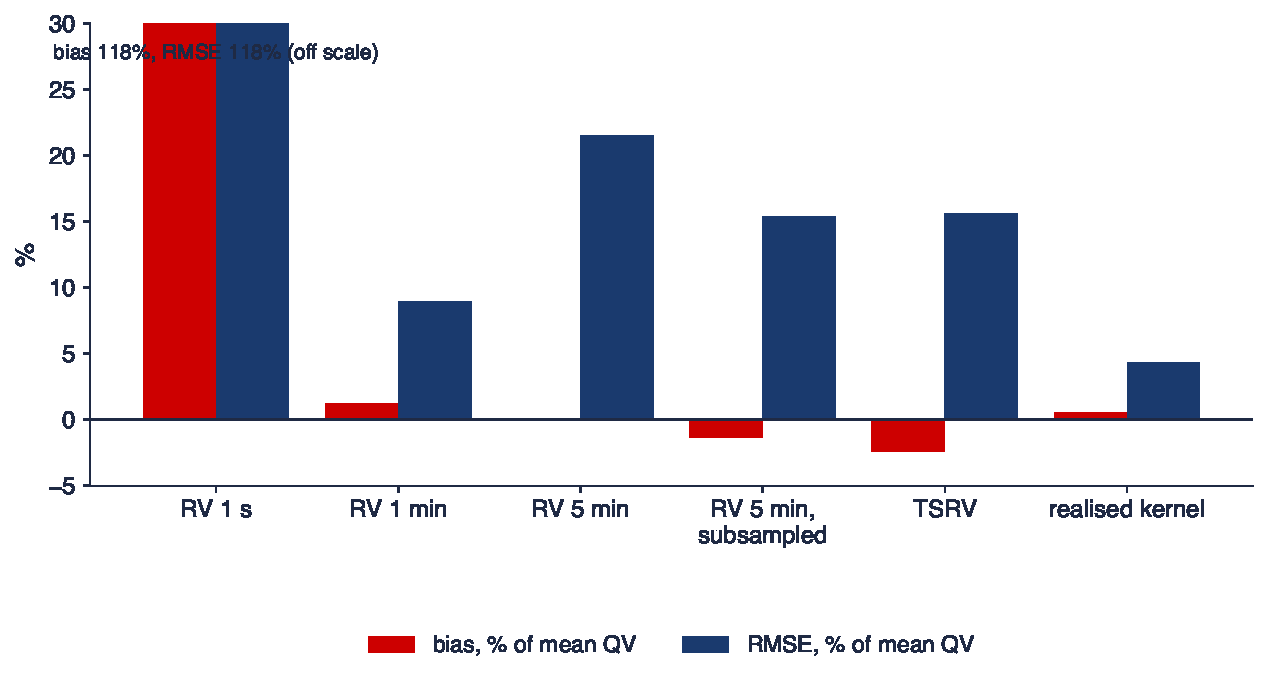
\includegraphics[width=0.97\textwidth,height=0.6\textheight,keepaspectratio]{ats_ch8_kernels.pdf}
\end{center}
\vspace{-0.25cm}
\begin{itemize}
    \item 300 de zile simulate cu salturi și zgomot; deplasarea și rădăcina erorii pătratice medii, relativ la media QV; TSRV cu $K = 300$ de secunde; RK cu lățimea de bandă BNHLS (mediana $H = 31$)
\end{itemize}
\quantlet{ATS\_ch8\_realised\_measures}{\qlurl{ATS_ch8_realised_measures}}
\end{frame}

\begin{frame}{Interpretarea comparației estimatorilor}
\itemsize{\small}
\begin{itemize}
    \item RV la o secundă este dominat de zgomot: deplasarea este 117{,}8\% din QV; la un minut deplasarea este 1{,}2\%, iar RMSE 8{,}9\%
    \item RV la cinci minute este nedeplasat, dar zgomotos (RMSE 21{,}6\%); subeșantionarea și TSRV îl reduc la 15{,}4\% și 15{,}6\%
    \item Realised kernel-ul folosește toate cele 23\,400 de randamente: deplasarea 0{,}5\%, RMSE 4{,}4\%, cel mai bun dintre cei șase
    \item Toți estimatorii de aici au ca țintă QV, inclusiv salturile; separarea salturilor cere secțiunea următoare
\end{itemize}
\end{frame}

\begin{frame}{Signature plot și efectul Epps: Bitcoin și Ether}
\itemsize{\footnotesize}
\begin{center}
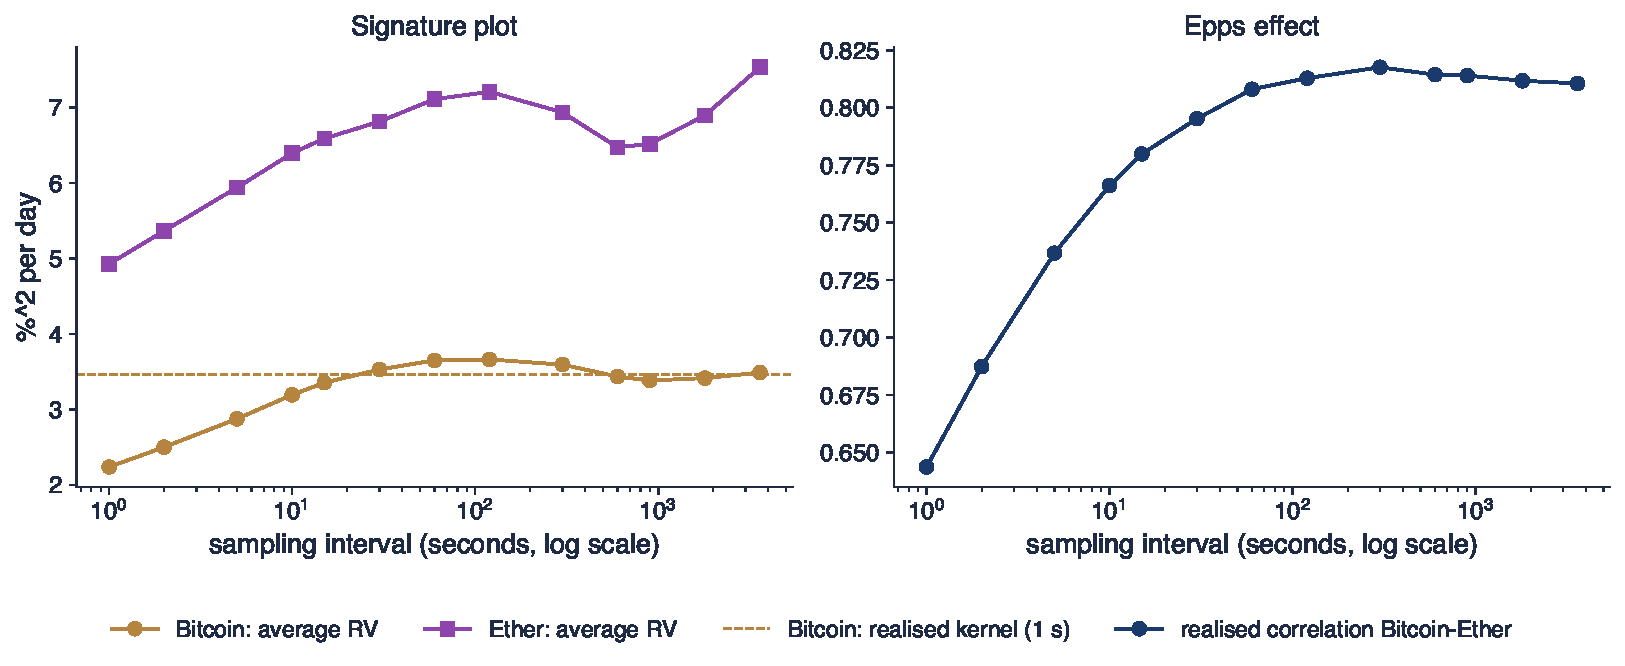
\includegraphics[width=0.97\textwidth,height=0.6\textheight,keepaspectratio]{ats_ch8_signature.pdf}
\end{center}
\vspace{-0.25cm}
\begin{itemize}
    \item Prețuri Binance la o secundă, august 2026 (31 de zile); RV zilnic mediu în funcție de intervalul de eșantionare (subeșantionat); corelația realizată a celor două monede în funcție de interval
\end{itemize}
\quantlet{ATS\_ch8\_realised\_measures}{\qlurl{ATS_ch8_realised_measures}}
\end{frame}

\begin{frame}{Interpretarea signature plot-ului}
\itemsize{\small}
\begin{itemize}
    \item Bitcoin: RV este 2{,}24 la o secundă, 3{,}65 la un minut, 3{,}59 la cinci minute: signature plot-ul \emph{crește}, opusul predicției pentru zgomot i.i.d.
    \item Motivul: 52\% dintre randamentele la o secundă sînt zero (nicio tranzacție sau același preț), iar prețurile se ajustează treptat, deci randamentele la o secundă sînt autocorelate pozitiv
    \item Realised kernel-ul pe date la o secundă (3{,}46, mediana $H = 22$) adaugă înapoi autocovarianțele pozitive și ajunge în zona plată de 1--30 de minute
    \item Efectul Epps \refEpp: corelația realizată 0{,}64 la o secundă față de 0{,}82 la cinci minute; tranzacționarea asincronă deplasează covarianțele spre zero la frecvență înaltă
\end{itemize}
\end{frame}

\begin{frame}{Recapitulare: măsurile realizate}
\itemsize{\small}
\begin{itemize}
    \item RV estimează QV cu eroarea $\sqrt{2\mathrm{IQ}/n}$; intervalul în logaritmi se comportă mai bine; convergența stabilă face validă studentizarea
    \item Zgomotul deplasează RV la frecvență înaltă; semnul și mărimea acestui efect sînt empirice: priviți întîi signature plot-ul
    \item Realised kernels folosesc toate datele și corectează zgomotul cu dependență pe distanțe scurte; RV la 5 minute rămîne un reper robust
\end{itemize}
\end{frame}


%=============================================================================
\section{Salturi: variația bipower și teste}
%=============================================================================

\begin{frame}{Variația bipower (1/2)}
\itemsize{\small}
\begin{itemize}
    \item \refBNSb: suma produselor valorilor absolute ale randamentelor adiacente, rescalată
    \[ \mathrm{BV}_t = \mu_1^{-2}\,\frac{n}{n-1}\sum_{i=2}^n\lvert r_{t,i}\rvert\,\lvert r_{t,i-1}\rvert, \qquad \mu_1 = \E|Z| = \sqrt{2/\pi} \]
    \begin{itemize}
        \item $Z \sim N(0, 1)$; $\mu_1^{-2}$ face $\mathrm{BV}_t$ consistent pentru $\mathrm{IV}_t$; $\frac{n}{n-1}$ corectează pentru cele $n-1$ produse
        \item $\mathrm{BV}_t \to \mathrm{IV}_t$ chiar și cu salturi (cu activitate finită): un salt intră doar în două produse, fiecare înmulțit cu un randament de ordinul $n^{-1/2}$
    \end{itemize}
    \item Deci $\mathrm{RV}_t - \mathrm{BV}_t \to \sum_{s \le 1}(\Delta J_s)^2$: o estimație neparametrică a variației din salturi a zilei
\end{itemize}
\end{frame}

\begin{frame}{Variația bipower (2/2): estimatori înrudiți}
\itemsize{\small}
\begin{itemize}
    \item Cuarticitatea robustă la salturi: cuarticitatea tripower
    \[ \mathrm{TQ}_t = n\,\mu_{4/3}^{-3}\,\frac{n}{n-2}\sum_{i=3}^n\prod_{j=0}^2|r_{t,i-j}|^{4/3}, \qquad \mu_{4/3} = \E|Z|^{4/3} \]
    \begin{itemize}
        \item produse a trei valori absolute ale randamentelor adiacente, fiecare la puterea $4/3$; $\mathrm{TQ}_t \to \mathrm{IQ}_t$ chiar și cu salturi (RQ, nu)
    \end{itemize}
    \item Trunchierea prin vecinii cei mai apropiați (MedRV, MinRV) \refADS: deplasare mai mică în eșantioane finite din cauza unui salt și a randamentelor nule
    \item RV cu prag (trunchiat): se elimină randamentele peste $c\,n^{-\varpi}$
    \begin{itemize}
        \item $c > 0$: o constantă (un multiplu al volatilității locale); $\varpi \in (0, \frac12)$: pragul scade mai lent decît un randament de difuzie, deci sînt eliminate doar salturile
    \end{itemize}
\end{itemize}
\end{frame}

\begin{frame}{Testarea salturilor (1/2): statistica raport}
\itemsize{\small}
\begin{itemize}
    \item \refBNSc: fără salturi, diferența RV $-$ BV este și ea mixt normală
    \[ \sqrt n(\mathrm{RV}_t - \mathrm{BV}_t) \to MN(0, \vartheta\,\mathrm{IQ}_t), \qquad \vartheta = \mu_1^{-4} + 2\mu_1^{-2} - 5 = \frac{\pi^2}{4} + \pi - 5 \approx 0{,}609 \]
    \begin{itemize}
        \item $\vartheta$: o constantă care măsoară cu cît este BV mai puțin eficient decît RV
    \end{itemize}
    \item Statistica raport \refHT: contribuția relativă a salturilor, studentizată
    \[ z_t = \frac{(\mathrm{RV}_t - \mathrm{BV}_t)/\mathrm{RV}_t}{\sqrt{\frac{\vartheta}{n}\max\big(1, \mathrm{TQ}_t/\mathrm{BV}_t^2\big)}} \to N(0, 1) \]
    \begin{itemize}
        \item test unilateral: respingem ipoteza „niciun salt în ziua $t$” pentru $z_t$ mare
        \item forma de raport și ajustarea prin max dau cea mai bună mărime a testului în simulările lor; $\mathrm{TQ}_t/\mathrm{BV}_t^2 \ge 1$ prin Jensen cînd volatilitatea variază în cursul zilei
    \end{itemize}
\end{itemize}
\end{frame}

\begin{frame}{Testarea salturilor (2/2): aplicarea practică}
\itemsize{\small}
\begin{itemize}
    \item Un test zilnic răspunde la întrebarea „a existat un salt azi?”; localizarea lui în cursul zilei cere un test pe fiecare randament standardizat cu BV local \refLM
    \item Testare multiplă: la nivelul $\alpha$, pe $T$ zile ne așteptăm la $\alpha T$ zile cu salturi false
    \begin{itemize}
        \item folosiți un $\alpha$ mic (0,1\%) sau o corecție de tip FWER sau FDR (\atschlink{https://danpele.github.io/Advanced-Time-Series/RO/Cursuri/capitol1_evaluarea_prognozelor.pdf}{Capitolul 1})
    \end{itemize}
    \item Separarea părților continuă și de salt ale lui RV \refABD
    \[ J_t = \mathbb 1(z_t > z_{1-\alpha})\,(\mathrm{RV}_t - \mathrm{BV}_t), \qquad C_t = \mathrm{RV}_t - J_t \]
    \begin{itemize}
        \item $\mathbb 1(\cdot)$: indicatorul, 1 dacă testul respinge și 0 altfel; $z_{1-\alpha}$: cuantila $1-\alpha$ a distribuției $N(0, 1)$
        \item $J_t$: partea de salt, nenulă doar în zilele semnificative; $C_t$: partea continuă
    \end{itemize}
\end{itemize}
\end{frame}

\begin{frame}{Mărimea și puterea testului raport}
\itemsize{\footnotesize}
\begin{center}
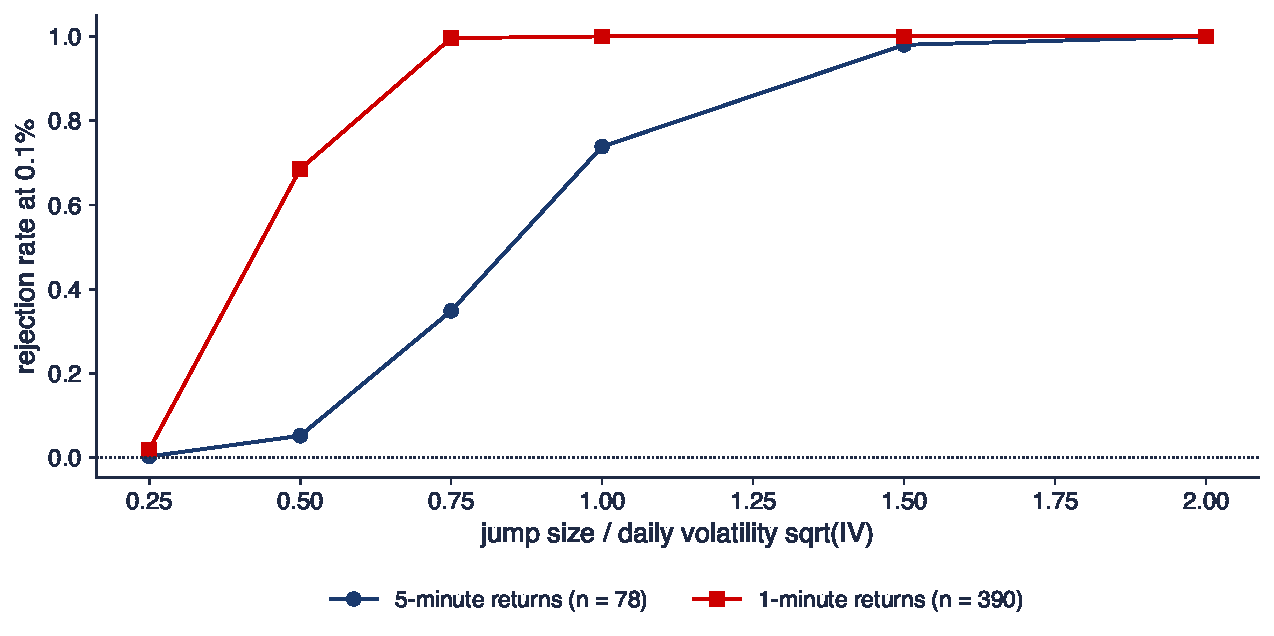
\includegraphics[width=0.97\textwidth,height=0.6\textheight,keepaspectratio]{ats_ch8_jump_power.pdf}
\end{center}
\vspace{-0.25cm}
\begin{itemize}
    \item 2\,000 de zile simulate (SV cu doi factori, fără salturi), apoi un salt de mărime $c\sqrt{\mathrm{IV}_t}$ la un moment aleator; test unilateral la 0,1\% cu randamente la 5 minute și la 1 minut
\end{itemize}
\quantlet{ATS\_ch8\_jumps}{\qlurl{ATS_ch8_jumps}}
\end{frame}

\begin{frame}{Interpretarea mărimii și puterii}
\itemsize{\small}
\begin{itemize}
    \item Mărimea fără salturi: 0{,}0\% (5 minute) și 0{,}2\% (1 minut) față de 0,1\% nominal; cu zgomot i.i.d. de mărimea calibrată, tot 0{,}1\% la 1 minut
    \item Puterea pentru un salt de o jumătate de abatere standard zilnică: 5\% cu randamente la 5 minute, 68\% cu randamente la 1 minut; pentru o abatere standard 74\% și 100\%
    \item Puterea depinde de $c\sqrt n$: salturile mici sînt absorbite în difuzie la o eșantionare rară (Seminarul 8, A6 dă pragul de detectare)
    \item Compromisul cu zgomotul este același ca pentru RV: o eșantionare mai fină crește puterea pînă cînd zgomotul și randamentele nule distorsionează statistica
\end{itemize}
\end{frame}

\begin{frame}{Zilele cu salturi pentru Bitcoin și Ether}
\itemsize{\footnotesize}
\begin{center}
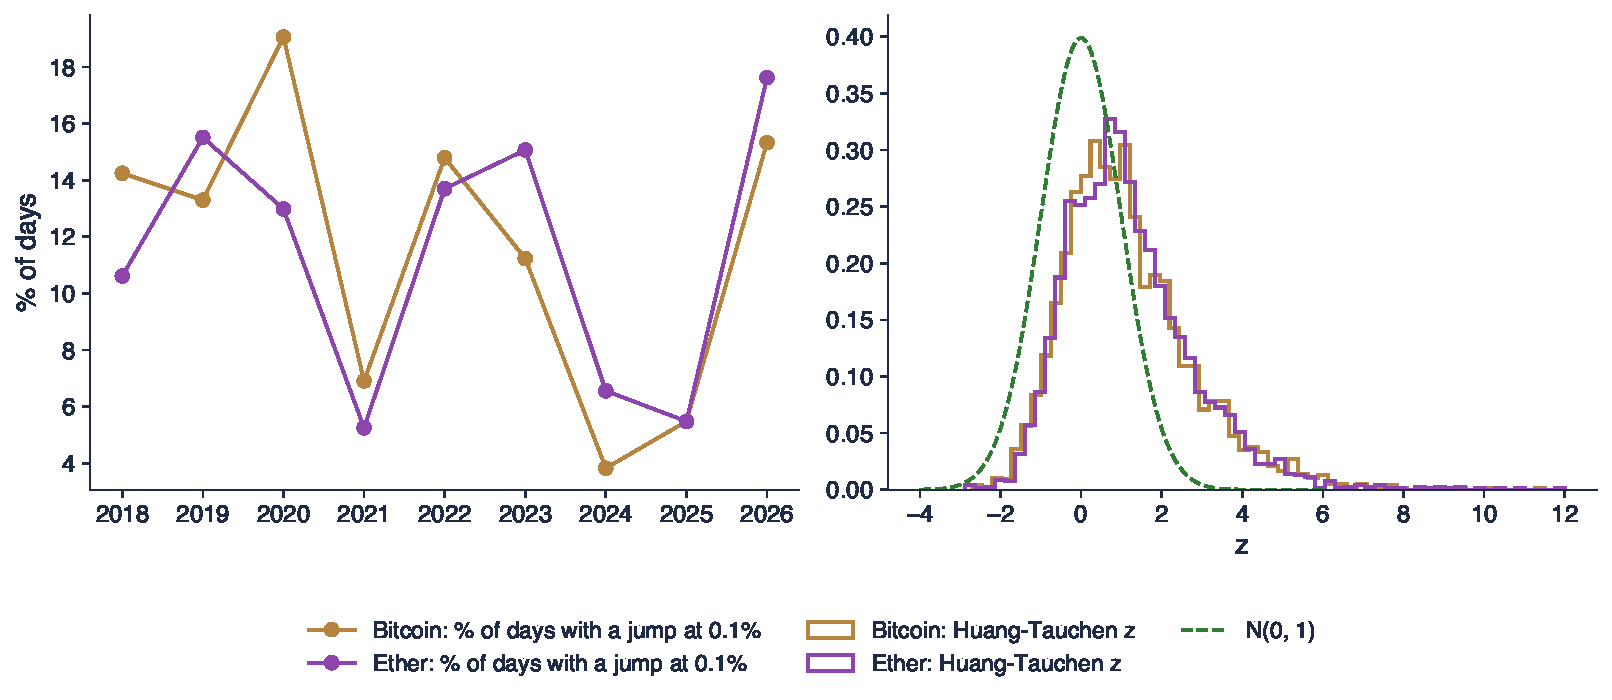
\includegraphics[width=0.97\textwidth,height=0.6\textheight,keepaspectratio]{ats_ch8_jumps_crypto.pdf}
\end{center}
\vspace{-0.25cm}
\begin{itemize}
    \item Testul Huang--Tauchen cu randamente la 5 minute ($n = 288$ pe zi UTC), 2018--2026, $T = 3\,165$ de zile; stînga: ponderea zilelor cu salturi la 0,1\% pe an; dreapta: distribuția lui $z_t$ față de $N(0, 1)$
\end{itemize}
\quantlet{ATS\_ch8\_jumps}{\qlurl{ATS_ch8_jumps}}
\end{frame}

\begin{frame}{Interpretarea testelor de salt pentru criptomonede}
\itemsize{\small}
\begin{itemize}
    \item Bitcoin: 362 de zile cu salturi (11{,}4\%), unde ne așteptăm la aproximativ 3{,}2 respingeri false; Ether: 355 de zile (11{,}2\%)
    \item Totuși, salturile sînt mici: reprezintă 3{,}0\% (Bitcoin) și 2{,}3\% (Ether) din variația totală; restul este continuu
    \item Întreaga distribuție a lui $z_t$ este deplasată (media 1{,}16, nu 0): pe lîngă salturi, sezonalitatea intraday pe 24 de ore, randamentele nule și mișcările bruște încalcă ipotezele nulei
    \item Înainte de a declara o zi drept zi cu salt: standardizați randamentele cu un profil al volatilității intraday, verificați randamentele nule și controlați numărul de teste
\end{itemize}
\end{frame}

\begin{frame}{Recapitulare: salturile}
\itemsize{\small}
\begin{itemize}
    \item BV estimează partea continuă; RV $-$ BV partea de salt; TQ face testul robust la salturi în cuarticitate
    \item Testul raport are o mărime bună în simulări; puterea lui crește cu $c\sqrt n$
    \item În datele reale, ipoteza nulă este fragilă: multe respingeri, puțină variație din salturi; tratați numărul de salturi ca dependent de model
\end{itemize}
\end{frame}


%=============================================================================
\section{Prognoza varianței realizate: HAR și HARQ}
%=============================================================================

\begin{frame}{Modelul HAR al lui Corsi (1/2): regresia}
\itemsize{\small}
\begin{itemize}
    \item \refCor: RV de mîine este o funcție liniară de mediile zilnică, săptămînală și lunară ale RV din trecut
    \[ \mathrm{RV}_{t+1} = \beta_0 + \beta_d\mathrm{RV}_t + \beta_w\mathrm{RV}^{(w)}_t + \beta_m\mathrm{RV}^{(m)}_t + u_{t+1} \]
    \[ \mathrm{RV}^{(w)}_t = \frac15\sum_{j=0}^4\mathrm{RV}_{t-j}, \qquad \mathrm{RV}^{(m)}_t = \frac1{22}\sum_{j=0}^{21}\mathrm{RV}_{t-j} \]
    \begin{itemize}
        \item $\mathrm{RV}^{(w)}_t$, $\mathrm{RV}^{(m)}_t$: mediile pe ultimele 5 zile de tranzacționare (o săptămînă) și pe ultimele 22 (o lună)
        \item $\beta_d, \beta_w, \beta_m \ge 0$: ponderile celor trei orizonturi; $\beta_0$: termenul liber; $u_{t+1}$: eroarea de prognoză, cu media zero
        \item $\beta_d + \beta_w + \beta_m$: persistența; cu cît este mai aproape de 1, cu atît volatilitatea revine mai lent la medie
    \end{itemize}
    \item Ipoteza pieței eterogene: participanții cu orizont zilnic, săptămînal și lunar reacționează la volatilitate la propriul orizont
    \begin{itemize}
        \item cascada produce autocorelații care scad lent
    \end{itemize}
\end{itemize}
\end{frame}

\begin{frame}{Modelul HAR al lui Corsi (2/2): estimare și variante}
\itemsize{\small}
\begin{itemize}
    \item Statistic, HAR este un AR(22) cu 19 restricții liniare (coeficienți în trepte)
    \begin{itemize}
        \item memorie scurtă, dar imită memoria lungă pe orizontul unei luni
    \end{itemize}
    \item OLS este consistent; erorile sînt heteroscedastice și, pentru ținte pe mai multe zile, suprapuse
    \begin{itemize}
        \item folosiți erorile standard Newey--West \refNW\ (HAC)
    \end{itemize}
    \item Variante
    \begin{itemize}
        \item log-HAR: aceeași regresie pe $\ln\mathrm{RV}$, cu erori aproape gaussiene; prognoza lui RV este $\exp(\hat\mu + \frac12\hat\sigma^2_u)$, cu $\hat\mu$ valoarea ajustată în logaritmi și $\hat\sigma^2_u$ varianța reziduurilor
        \item HAR pe $\sqrt{\mathrm{RV}}$; ținte pe $h$ zile (RV mediu pe următoarele $h$ zile)
    \end{itemize}
    \item Extensii: părțile continuă și de salt, HAR-CJ \refABD; semivarianțele pozitivă și negativă \refPS; volatilitatea implicită; termeni de levier
\end{itemize}
\end{frame}

\begin{frame}{HAR ca AR(22) restricționat}
\itemsize{\footnotesize}
\begin{center}
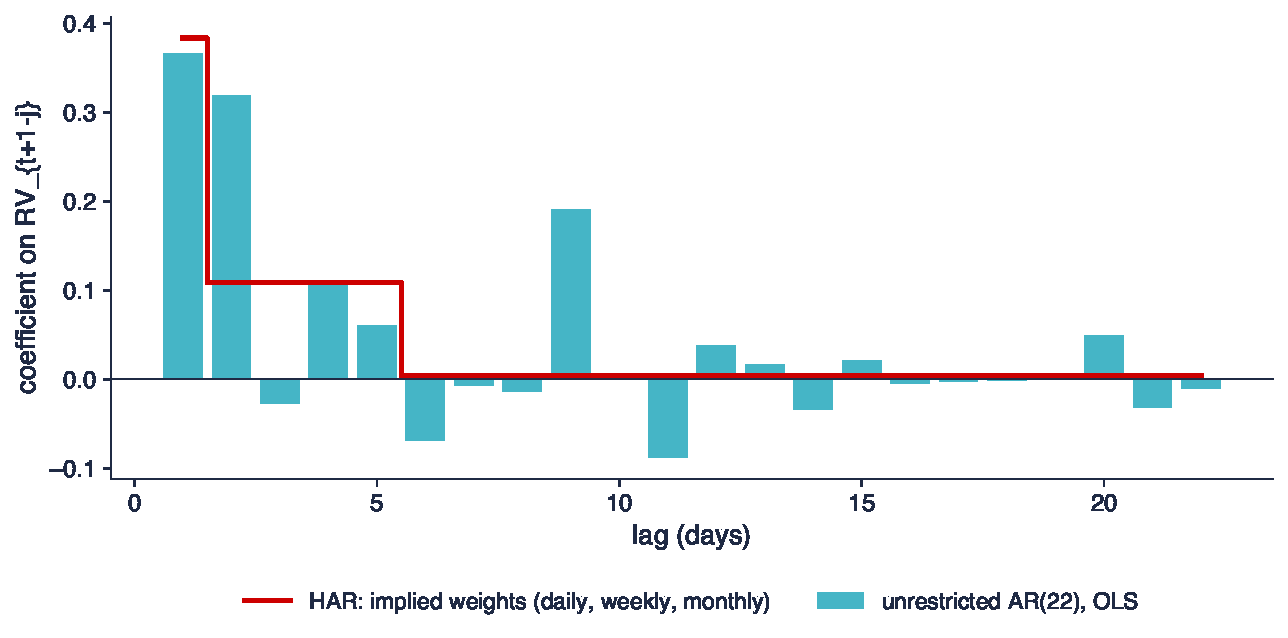
\includegraphics[width=0.97\textwidth,height=0.6\textheight,keepaspectratio]{ats_ch8_har_weights.pdf}
\end{center}
\vspace{-0.25cm}
\begin{itemize}
    \item S\&P 500 (Oxford-Man, RV la 5 minute, 2000--2022, $T = 5\,530$): coeficienții unui AR(22) nerestricționat estimat prin OLS și ponderile în trepte implicate de estimațiile HAR
\end{itemize}
\quantlet{ATS\_ch8\_har}{\qlurl{ATS_ch8_har}}
\end{frame}

\begin{frame}{Interpretarea estimațiilor HAR}
\itemsize{\small}
\begin{itemize}
    \item HAR: $\hat\beta_d = 0{,}275$ (0{,}104), $\hat\beta_w = 0{,}522$ (0{,}140), $\hat\beta_m = 0{,}094$ (0{,}078), erori standard Newey--West; $R^2 = 0{,}560$; persistența $\sum\hat\beta = 0{,}891$
    \item AR(22) cu 23 de coeficienți ajunge la $R^2 = 0{,}596$ în eșantion, cu coeficienți neregulați; HAR surprinde forma cu 4
    \item Log-HAR: $\hat\beta_d = 0{,}393$, $\hat\beta_w = 0{,}399$, $\hat\beta_m = 0{,}153$, $R^2 = 0{,}719$ pe $\ln\mathrm{RV}$; în logaritmi, componenta lunară contează mai mult
    \item În nivel, cîteva zile de criză domină OLS: erori standard mari pentru $\beta_d$ și $\beta_m$; metoda celor mai mici pătrate ponderate sau logaritmii dau estimații mai stabile
\end{itemize}
\end{frame}

\begin{frame}{Schema de prognoză}
\itemsize{\small}
\begin{itemize}
    \item Un pas înainte, fereastră mobilă de 1\,000 de zile, reestimare zilnică; ținta $\mathrm{RV}_{t+1}$
    \item Funcțiile de pierdere: MSE $= (\mathrm{RV} - f)^2$ și QLIKE, ambele robuste la zgomotul din RV (vezi mai jos)
    \[ \mathrm{QLIKE} = \frac{\mathrm{RV}}{f} - \ln\frac{\mathrm{RV}}{f} - 1 \ge 0 \]
    \begin{itemize}
        \item $f$: prognoza varianței; QLIKE este 0 cînd $f = \mathrm{RV}$ și penalizează subestimarea mai mult decît supraestimarea
    \end{itemize}
    \item Filtrul de plauzibilitate („insanity filter”) \refBPQ: o prognoză din afara intervalului RV din eșantionul de estimare este înlocuită cu media din eșantion
    \begin{itemize}
        \item prognozele liniare de tip HAR pot fi negative după un vîrf; QLIKE nu mai este atunci definită
        \item filtrul face parte din metodă și trebuie raportat
    \end{itemize}
    \item Statistica $t$ Diebold--Mariano \refDM\ pentru diferența pierderilor față de HAR
    \begin{itemize}
        \item varianță Newey--West; negativă = mai bun decît HAR, sub $-1{,}96$ semnificativ la 5\%; mai multe modele: setul de modele de încredere \refHLN, \atschlink{https://danpele.github.io/Advanced-Time-Series/RO/Cursuri/capitol1_evaluarea_prognozelor.pdf}{Capitolul 1}
    \end{itemize}
    \item Modele: HAR, HAR-CJ (partea continuă și partea de salt, din BV), log-HAR; pentru Bitcoin și Ether și HARQ
\end{itemize}
\end{frame}

\begin{frame}{Extensiile HAR în afara eșantionului}
\itemsize{\footnotesize}
\begin{center}
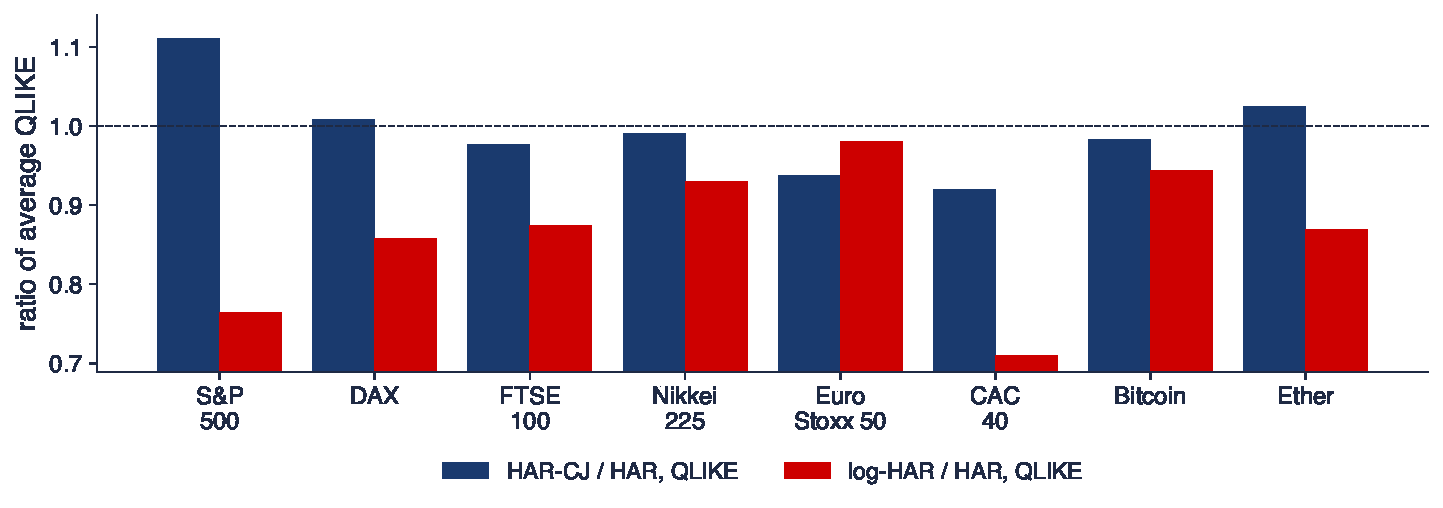
\includegraphics[width=0.97\textwidth,height=0.6\textheight,keepaspectratio]{ats_ch8_har_oos.pdf}
\end{center}
\vspace{-0.25cm}
\begin{itemize}
    \item QLIKE mediu relativ la HAR (sub 1 = mai bun), șase indici Oxford-Man (2004--2022) și două criptomonede (din 01.11.2020); fereastră mobilă de 1\,000 de zile
\end{itemize}
\quantlet{ATS\_ch8\_har}{\qlurl{ATS_ch8_har}}
\end{frame}

\begin{frame}{Interpretarea comparației HAR în afara eșantionului}
\itemsize{\small}
\begin{itemize}
    \item Log-HAR este mai bun decît HAR după QLIKE pentru 6 din 6 indici: S\&P 500 0{,}764 (DM \ensuremath{-}2{,}07), CAC 40 0{,}709 (DM \ensuremath{-}1{,}73), FTSE 0{,}874 (DM \ensuremath{-}5{,}08)
    \item HAR-CJ ajută pentru 4 din 6 indici, dar nu pentru S\&P 500 (1{,}110): separarea salturilor adaugă zgomot de estimare cînd salturile sînt mici
    \item Ordinea depinde de funcția de pierdere: după MSE, cîștigurile log-HAR sînt mai mici (S\&P 500: 0{,}837); MSE pune cea mai mare pondere pe zilele de criză
    \item Șase indici de la un singur furnizor de date și o singură perioadă: raportați-i pe toți, nu doar pe cel mai bun (data snooping, \atschlink{https://danpele.github.io/Advanced-Time-Series/RO/Cursuri/capitol1_evaluarea_prognozelor.pdf}{Capitolul 1})
\end{itemize}
\end{frame}

\begin{frame}{HARQ (1/2): eroarea de măsurare a lui RV}
\itemsize{\small}
\begin{itemize}
    \item RV este IV latent plus o eroare de măsurare a cărei varianță se schimbă în fiecare zi
    \[ \mathrm{RV}_t = \mathrm{IV}_t + e_t, \qquad \Var(e_t | \mathrm{IQ}_t) \approx \frac{2\,\mathrm{IQ}_t}{n} \]
    \begin{itemize}
        \item $e_t$: eroarea de măsurare din ziua $t$; în zilele volatile ($\mathrm{IQ}_t$ mare), RV este mai puțin precis
    \end{itemize}
    \item Erori în variabile: într-un AR(1) pentru IV cu coeficientul $\phi$, panta OLS pe RV este atenuată (\atsapplink{atsapp3}{atssrc3}{Anexa})
    \[ \mathrm{plim}\,\hat\phi = \phi\lambda, \qquad \lambda = \frac{\Var(\mathrm{IV})}{\Var(\mathrm{IV}) + \E\Var(e)} \in (0, 1) \]
    \begin{itemize}
        \item $\lambda$: raportul de fiabilitate, ponderea semnalului în varianța lui RV
        \item un singur $\beta_d$ constant este un compromis: prea mare în zilele zgomotoase, prea mic în zilele precise
    \end{itemize}
\end{itemize}
\end{frame}

\begin{frame}{HARQ (2/2): o pondere care depinde de precizie}
\itemsize{\small}
\begin{itemize}
    \item \refBPQ: ponderea RV de ieri variază cu precizia lui estimată
    \[ \mathrm{RV}_{t+1} = \beta_0 + \big(\beta_d + \beta_{dQ}\sqrt{\mathrm{RQ}_t}\big)\mathrm{RV}_t + \beta_w\mathrm{RV}^{(w)}_t + \beta_m\mathrm{RV}^{(m)}_t + u_{t+1} \]
    \begin{itemize}
        \item $\mathrm{RQ}_t$: cuarticitatea realizată, estimația lui $\mathrm{IQ}_t$; $\sqrt{\mathrm{RQ}_t}$ este proporțional cu abaterea standard a lui $e_t$
        \item ne așteptăm la $\beta_{dQ} < 0$: cu cît RV de ieri este mai puțin precis, cu atît ponderea lui este mai mică
        \item $\sqrt{\mathrm{RQ}_t}$ este centrat, astfel încît $\beta_d$ este ponderea unei zile cu precizie medie
    \end{itemize}
    \item Un singur parametru în plus, tot OLS
    \item Lucrarea originală: futures pe S\&P 500 și 27 de acțiuni din Dow Jones, cîștiguri față de HAR în eșantion și în afara lui
    \begin{itemize}
        \item replicarea noastră o extinde la Bitcoin și Ether, 2018--2026, unde RQ este disponibil din datele noastre la un minut
    \end{itemize}
\end{itemize}
\end{frame}

\begin{frame}{HARQ pentru Bitcoin: o pondere care se schimbă cu precizia}
\itemsize{\footnotesize}
\begin{center}
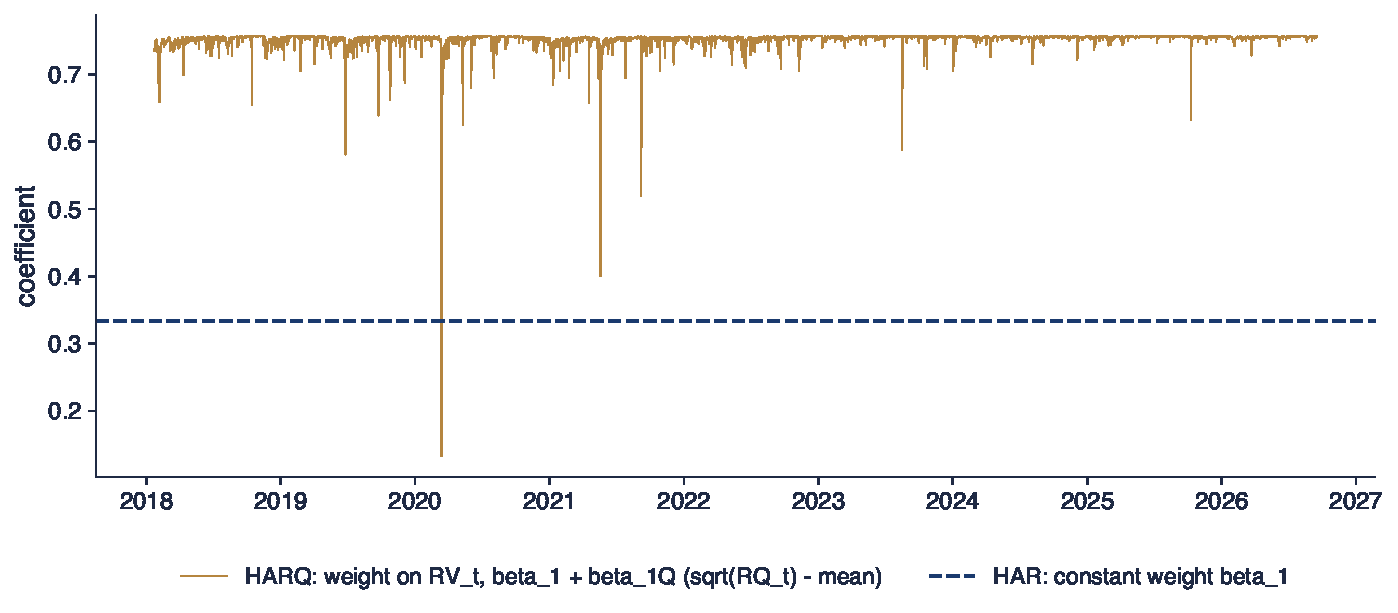
\includegraphics[width=0.97\textwidth,height=0.6\textheight,keepaspectratio]{ats_ch8_harq.pdf}
\end{center}
\vspace{-0.25cm}
\begin{itemize}
    \item HARQ pe tot eșantionul, pentru RV și RQ la 5 minute ale Bitcoin: ponderea zilnică $\hat\beta_d + \hat\beta_{dQ}(\sqrt{\mathrm{RQ}_t} - \overline{\sqrt{\mathrm{RQ}}})$ față de ponderea constantă din HAR
\end{itemize}
\quantlet{ATS\_ch8\_har}{\qlurl{ATS_ch8_har}}
\end{frame}

\begin{frame}{Interpretarea modelului HARQ}
\itemsize{\small}
\begin{itemize}
    \item $\hat\beta_{dQ} = \ensuremath{-}0{,}00021$ ($t = \ensuremath{-}2{,}7$, Newey--West): negativ, cum prezice teoria; ponderea zilnică la precizie medie este 0{,}752, față de 0{,}334 în HAR
    \item În majoritatea zilelor ponderea este în jur de 0{,}76; în zilele cele mai zgomotoase scade (cuantila de 1\% 0{,}71, minimul 0{,}13): RV de ieri primește încredere doar cînd este precis
    \item În afara eșantionului, QLIKE relativ la HAR: Bitcoin 0{,}946 (DM \ensuremath{-}2{,}44), Ether 0{,}921 (DM \ensuremath{-}4{,}50): cîștigul din studiul original se regăsește la criptomonede
    \item După MSE imaginea diferă (Bitcoin 1{,}163): MSE este dominat de cîteva zile extreme, unde HARQ micșorează cel mai mult ponderea; mini studiul de caz AI verifică cît de fragil este cîștigul
\end{itemize}
\end{frame}

\begin{frame}{Recapitulare: HAR și HARQ}
\itemsize{\small}
\begin{itemize}
    \item HAR este un AR(22) restricționat și parcimonios, estimat prin OLS; logaritmii îl stabilizează
    \item Cîștigurile în afara eșantionului depind de funcția de pierdere și de piață: raportați toate seriile, filtrul și testele DM
    \item HARQ lasă eroarea de măsurare a RV să stabilească ponderea zilei de ieri: un parametru, un cîștig robust după QLIKE
\end{itemize}
\end{frame}


%=============================================================================
\section{Realized GARCH și HEAVY}
%=============================================================================

\begin{frame}{Realized GARCH (1/2): cele trei ecuații}
\itemsize{\footnotesize}
\begin{itemize}
    \item \refHHS, forma log-liniară: o ecuație a randamentului, o ecuație GARCH determinată de măsura realizată și o ecuație de măsurare
    \[ r_t = \sqrt{h_t}\,z_t, \qquad \ln h_t = \omega + \beta\ln h_{t-1} + \gamma\ln x_{t-1} \]
    \[ \ln x_t = \xi + \varphi\ln h_t + \tau(z_t) + u_t \]
    \begin{itemize}
        \item $h_t$: varianța condiționată a randamentului $r_t$; $z_t$: șoc standardizat i.i.d.; $x_t$: măsura realizată din ziua $t$ (aici realised kernel-ul RK)
        \item $\beta$: persistența lui $\ln h_t$; $\gamma$: ponderea măsurii realizate de ieri (variabila de știri care înlocuiește $\varepsilon^2_{t-1}$)
        \item $u_t$: eroarea de măsurare, i.i.d. $N(0, \sigma^2_u)$, independentă de $z_t$
    \end{itemize}
    \item Ecuația de măsurare: $x_t$ este un semnal zgomotos, posibil deplasat, al lui $h_t$
    \begin{itemize}
        \item $\varphi = 1$: $x_t$ proporțional cu $h_t$; $\xi$ preia diferența de scală (măsura deschidere--închidere față de varianța închidere--închidere)
        \item funcția de levier $\tau(z) = \tau_1z + \tau_2(z^2 - 1)$: cu $\tau_1 < 0$, randamentele negative cresc următoarea măsură realizată (impactul știrilor, \atschlink{https://danpele.github.io/Time-Series-Analysis/RO/Cursuri/capitol5_volatilitate_conditionata_garch.pdf}{TSA, Capitolul 5})
    \end{itemize}
\end{itemize}
\end{frame}

\begin{frame}{Realized GARCH (2/2): forma redusă și estimarea}
\itemsize{\small}
\begin{itemize}
    \item Înlocuind ecuația de măsurare în ecuația GARCH: $\ln h_t$ este un AR(1)
    \[ \ln h_t = (\omega + \gamma\xi) + \pi\ln h_{t-1} + \gamma\big(\tau(z_{t-1}) + u_{t-1}\big), \qquad \pi = \beta + \varphi\gamma \]
    \begin{itemize}
        \item $\pi$: persistența logaritmului varianței; prognozele cu mai mulți pași decurg din ea, pentru că $x_t$ are propria ecuație
    \end{itemize}
    \item QML comun: log-verosimilitatea însumează o parte pentru randamente și o parte pentru măsurare
    \[ \ell = -\frac12\sum_t\Big[\underbrace{\ln h_t + z_t^2}_{r_t} + \underbrace{\ln\sigma^2_u + u_t^2/\sigma^2_u}_{x_t}\Big] \]
    \begin{itemize}
        \item comparația cu GARCH se face doar prin verosimilitatea parțială a lui $r_t$ (prima parte), deoarece GARCH nu modelează $x_t$
    \end{itemize}
\end{itemize}
\end{frame}

\begin{frame}{HEAVY și familia modelelor cu măsuri realizate}
\itemsize{\footnotesize}
\begin{itemize}
    \item HEAVY \refSS: două ecuații de tip GARCH, una pentru varianța randamentului și una pentru media măsurii realizate
    \[ h_t = \Var(r_t | \mathcal F_{t-1}) = \omega + \alpha\mathrm{RM}_{t-1} + \beta h_{t-1} \]
    \[ \mu_t = \E(\mathrm{RM}_t | \mathcal F_{t-1}) = \omega_R + \alpha_R\mathrm{RM}_{t-1} + \beta_R\mu_{t-1} \]
    \begin{itemize}
        \item $\mathrm{RM}_t$: măsura realizată din ziua $t$; $(\omega, \alpha, \beta)$ și $(\omega_R, \alpha_R, \beta_R)$: parametrii celor două ecuații
        \item fiecare ecuație se estimează separat prin QML; „momentum”: după un șoc, $h_t$ continuă să crească pînă cînd $\mu_t$ îl ajunge din urmă
        \item cînd măsura realizată intră în ecuația varianței, pătratul randamentului de obicei nu mai adaugă nimic ($\varepsilon^2_{t-1}$ primește coeficientul zero)
    \end{itemize}
    \item Realized EGARCH \refHH: mai multe măsuri realizate și un efect de levier mai bogat; există versiuni de tip score-driven pentru cozi groase
    \item Comparativ cu HAR: randamentele și măsurile realizate sînt modelate împreună, deci sînt disponibile prognoze de densitate și de VaR/ES (\atschlink{https://danpele.github.io/Advanced-Time-Series/RO/Cursuri/capitol9_var_es_backtesting.pdf}{Capitolul 9})
\end{itemize}
\end{frame}

\begin{frame}{Studiu de caz: Realized GARCH pentru S\&P 500}
\itemsize{\footnotesize}
\begin{center}
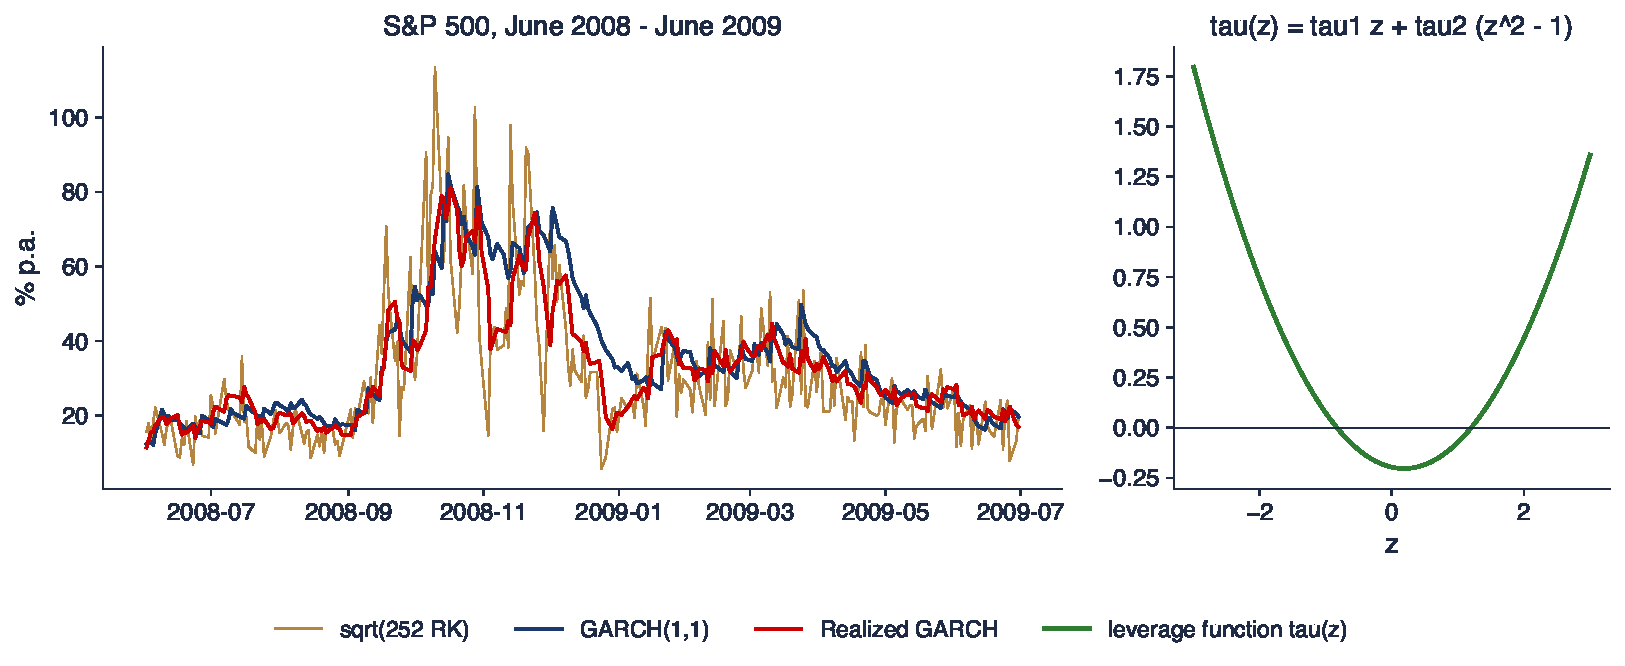
\includegraphics[width=0.97\textwidth,height=0.6\textheight,keepaspectratio]{ats_ch8_rgarch.pdf}
\end{center}
\vspace{-0.25cm}
\begin{itemize}
    \item Randamente deschidere--închidere și realised kernel-ul Parzen (Oxford-Man), 2000--2022, $T = 5\,552$, ca în \refHHS; stînga: criza din 2008; dreapta: funcția de levier estimată
\end{itemize}
\quantlet{ATS\_ch8\_realized\_garch}{\qlurl{ATS_ch8_realized_garch}}
\end{frame}

\begin{frame}{Estimațiile Realized GARCH}
\itemsize{\small}
\begin{center}
\footnotesize
\begin{tabular}{cccccccc}
\toprule
$\omega$ & $\beta$ & $\gamma$ & $\xi$ & $\varphi$ & $\tau_1$ & $\tau_2$ & $\sigma_u$ \\
\midrule
0{,}119 & 0{,}678 & 0{,}287 & \ensuremath{-}0{,}456 & 1{,}012 & \ensuremath{-}0{,}073 & 0{,}197 & 0{,}671 \\
(0{,}010) & (0{,}018) & (0{,}016) & (0{,}021) & (0{,}026) & (0{,}008) & (0{,}010) & (0{,}008) \\
\bottomrule
\end{tabular}
\end{center}
\begin{itemize}
    \item Erori standard Bollerslev--Wooldridge în paranteze; persistența $\hat\pi = \hat\beta + \hat\varphi\hat\gamma = 0{,}968$ (GARCH(1,1) pe aceleași randamente: 0{,}989)
    \item Log-verosimilitatea parțială a randamentelor: Realized GARCH \ensuremath{-}6899{,}7, HEAVY \ensuremath{-}6902{,}8, GJR \ensuremath{-}6998{,}8, GARCH(1,1) \ensuremath{-}7099{,}0
    \item Ecuația varianței HEAVY: $\hat\alpha = 0{,}377$ pentru $\mathrm{RK}_{t-1}$, $\hat\beta = 0{,}691$
\end{itemize}
\end{frame}

\begin{frame}{Interpretarea modelului Realized GARCH}
\itemsize{\small}
\begin{itemize}
    \item $\hat\varphi = 1{,}012$: kernel-ul este proporțional cu varianța condiționată; $\hat\xi = \ensuremath{-}0{,}456$, cu $\hat\sigma_u = 0{,}671$: în medie, kernel-ul se află sub varianța condiționată a randamentului deschidere--închidere
    \item $\hat\gamma = 0{,}287$ este mare, iar $\hat\beta = 0{,}678$ mai mic decît în GARCH: măsura realizată aduce informația mai repede decît pătratele randamentelor (panoul din stînga, toamna lui 2008)
    \item Levierul: $\hat\tau_1 = \ensuremath{-}0{,}073$, $\hat\tau_2 = 0{,}197$: o parabolă asimetrică, mai mare pentru $z$ negativ
    \item Cîștigul în verosimilitatea parțială față de GARCH(1,1), egal cu 199{,}3, are direcția din lucrarea originală; HEAVY este aproape la fel de bun, cu trei parametri
\end{itemize}
\end{frame}

\begin{frame}{Recapitulare: modelele GARCH cu măsuri realizate}
\itemsize{\small}
\begin{itemize}
    \item O măsură realizată în ecuația varianței este o variabilă de știri mai bună decît pătratul randamentului
    \item Realized GARCH adaugă o ecuație de măsurare: prognoze cu mai mulți pași, levier și o verosimilitate comună
    \item Comparația cu GARCH se face doar pe verosimilitatea parțială a randamentelor
\end{itemize}
\end{frame}


%=============================================================================
\section{Evaluarea prognozelor de volatilitate față de o țintă zgomotoasă}
%=============================================================================

\begin{frame}{Problema proxy-ului și funcțiile de pierdere robuste (1/2)}
\itemsize{\small}
\begin{itemize}
    \item Nu observăm niciodată $\sigma^2_t$: o prognoză $h_t$ este comparată cu un proxy $\hat\sigma^2_t$ (pătratul randamentului, RV, RK)
    \begin{itemize}
        \item proxy-ul este nedeplasat condiționat, $\E(\hat\sigma^2_t | \mathcal F_{t-1}) = \sigma^2_t$, dar zgomotos
    \end{itemize}
    \item O funcție de pierdere $L$ este \emph{robustă} \refPat\ dacă ordinea prognozelor după $\E L(\hat\sigma^2_t, h_t)$ coincide cu ordinea după $\E L(\sigma^2_t, h_t)$, pentru orice proxy nedeplasat \refHLb
    \item Condiția necesară și suficientă: o formă Bregman (\atschlink{https://danpele.github.io/Advanced-Time-Series/RO/Cursuri/capitol1_evaluarea_prognozelor.pdf}{Capitolul 1}, funcții de scor consistente pentru medie)
    \[ L(\hat\sigma^2, h) = \tilde C(h) + B(\hat\sigma^2) + C(h)(\hat\sigma^2 - h), \qquad C'(h) < 0 \]
    \begin{itemize}
        \item $C$: o funcție descrescătoare de prognoză; $\tilde C$: primitiva ei, $\tilde C' = C$; $B$: orice funcție doar de proxy (nu influențează ordinea)
    \end{itemize}
\end{itemize}
\end{frame}

\begin{frame}{Problema proxy-ului și funcțiile de pierdere robuste (2/2)}
\itemsize{\small}
\begin{itemize}
    \item Robuste: MSE și QLIKE, membrii de grad 2 și de grad 0 ai familiei omogene robuste
    \[ \mathrm{MSE} = (\hat\sigma^2 - h)^2, \qquad \mathrm{QLIKE} = \frac{\hat\sigma^2}{h} - \ln\frac{\hat\sigma^2}{h} - 1 \]
    \begin{itemize}
        \item gradul: cum se scalează pierderea cînd proxy-ul și prognoza sînt înmulțite cu aceeași constantă; QLIKE (grad 0) nu depinde de scală și penalizează mai mult subestimarea
    \end{itemize}
    \item Nerobuste: MAE $= |\hat\sigma^2 - h|$, MSE pe logaritmi $(\ln\hat\sigma^2 - \ln h)^2$, MSE pe abateri standard
    \begin{itemize}
        \item cu un proxy zgomotos, ele recompensează prognozele deplasate în jos
    \end{itemize}
    \item Exemplu: cu $\hat\sigma^2 = r^2$, optimul MSE-log este $h^* = \exp(\E\ln r^2) = 0{,}28\,\sigma^2$
    \begin{itemize}
        \item pentru că $r^2 = \sigma^2\chi^2_1$ pentru un randament gaussian, iar $\E\ln\chi^2_1 = -1{,}27$: MSE-log preferă o prognoză mult sub valoarea adevărată
    \end{itemize}
\end{itemize}
\end{frame}

\begin{frame}{Funcții de pierdere robuste și nerobuste}
\itemsize{\footnotesize}
\begin{center}
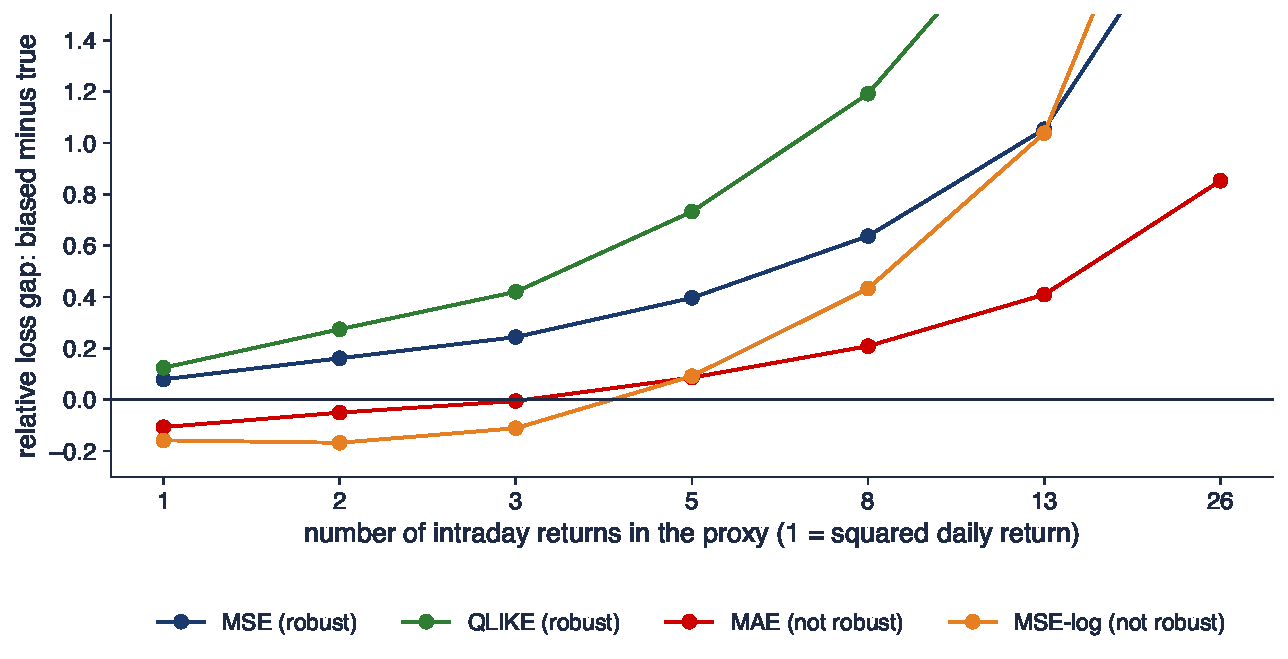
\includegraphics[width=0.97\textwidth,height=0.6\textheight,keepaspectratio]{ats_ch8_patton.pdf}
\end{center}
\vspace{-0.25cm}
\begin{itemize}
    \item Varianța adevărată față de o prognoză deplasată în jos cu factorul 0{,}6; proxy = RV din $n$ randamente intraday ($n = 1$: pătratul randamentului zilnic); diferența relativă a pierderilor așteptate, peste zero = cîștigă varianța adevărată
\end{itemize}
\quantlet{ATS\_ch8\_robust\_loss}{\qlurl{ATS_ch8_robust_loss}}
\end{frame}

\begin{frame}{Interpretarea experimentului de robustețe}
\itemsize{\small}
\begin{itemize}
    \item Cu pătratul randamentului ca proxy, MAE preferă prognoza deplasată (diferența \ensuremath{-}10{,}7\%) la fel ca MSE-log (\ensuremath{-}15{,}8\%); MSE (7{,}9\%) și QLIKE (12{,}5\%) nu
    \item Cu $n = 5$ randamente intraday, toate cele patru funcții ordonează corect: un proxy precis face funcțiile nerobuste „aproape” robuste \refHLb
    \item Pericolul este cel mai mare exact acolo unde nu există măsuri realizate: date zilnice, piețe emergente, istorii lungi
    \item Regula: evaluați prognozele de volatilitate cu QLIKE (și MSE), față de cel mai bun proxy disponibil
\end{itemize}
\end{frame}

\begin{frame}{Șapte prognoze ale volatilității S\&P 500}
\itemsize{\footnotesize}
\begin{center}
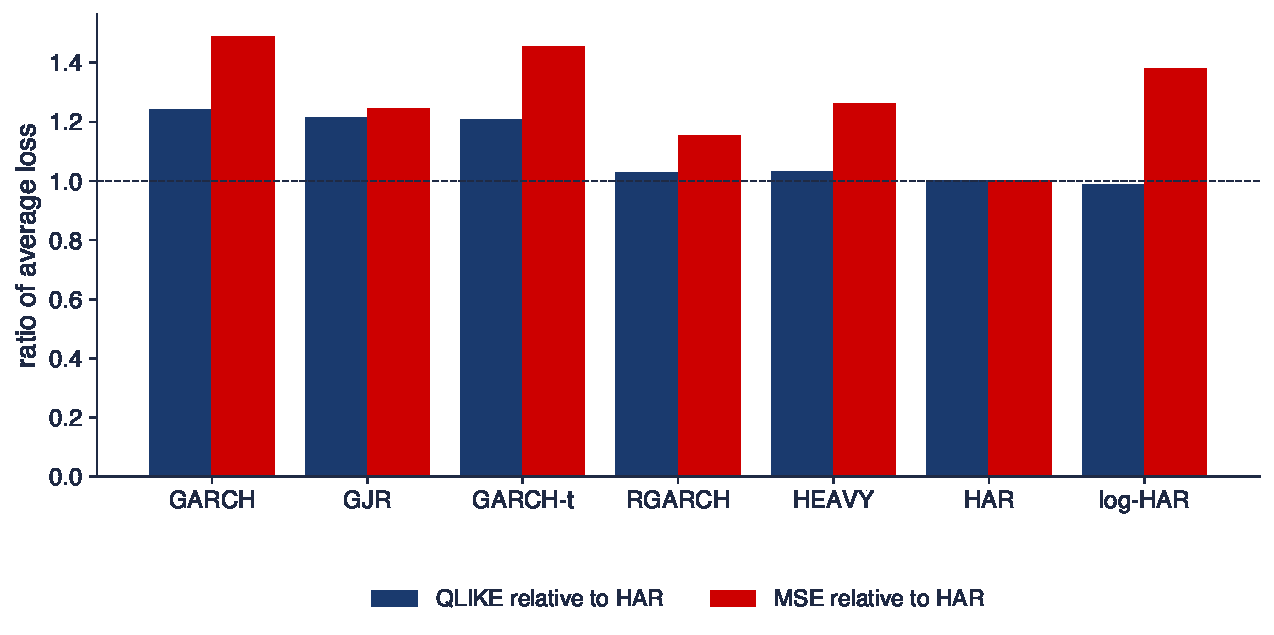
\includegraphics[width=0.97\textwidth,height=0.6\textheight,keepaspectratio]{ats_ch8_vol_oos.pdf}
\end{center}
\vspace{-0.25cm}
\begin{itemize}
    \item Varianța deschidere--închidere, un pas înainte, 2016--2022 ($1\,537$ zile); fereastră extinsă din 2000, parametrii reestimați la fiecare 250 de zile; proxy: realised kernel
\end{itemize}
\quantlet{ATS\_ch8\_robust\_loss}{\qlurl{ATS_ch8_robust_loss}}
\end{frame}

\begin{frame}{Interpretarea comparației prognozelor}
\itemsize{\small}
\begin{itemize}
    \item QLIKE: HAR 0{,}328, log-HAR 0{,}324, Realized GARCH 0{,}337, HEAVY 0{,}339, GARCH-$t$ 0{,}396, GJR 0{,}398, GARCH 0{,}407
    \item DM față de HAR (QLIKE): GARCH 8{,}62, GJR 6{,}27, Realized GARCH 1{,}42, log-HAR \ensuremath{-}0{,}37: modelele cu măsuri realizate sînt clar mai bune decît cele doar cu randamente; între ele diferențele sînt mici
    \item După MSE, HAR (1{,}60) conduce, iar statisticile DM sînt mai mici: crahul din 2020 domină erorile pătratice
    \item Un singur proxy (RK) pentru toate modelele: familia HAR este estimată pe aceeași măsură, ceea ce o avantajează; o comparație corectă încearcă și alt proxy (RV, BV)
\end{itemize}
\end{frame}

\begin{frame}{Recapitulare: evaluarea}
\itemsize{\small}
\begin{itemize}
    \item Doar funcțiile din clasa Patton păstrează ordinea cu un proxy nedeplasat zgomotos: MSE și QLIKE
    \item La un pas, modelele cu măsuri realizate depășesc modelele GARCH care folosesc doar randamentele; DM și MCS din \atschlink{https://danpele.github.io/Advanced-Time-Series/RO/Cursuri/capitol1_evaluarea_prognozelor.pdf}{Capitolul 1} cuantifică diferența
    \item Precizați proxy-ul, funcția de pierdere, fereastra și filtrul: fiecare poate schimba ordinea
\end{itemize}
\end{frame}


%=============================================================================
\section{GARCH multivariat și matrice de covarianță mari}
%=============================================================================

\begin{frame}{De la o varianță la o matrice de covarianță (1/2)}
\itemsize{\small}
\begin{itemize}
    \item Vectorul celor $N$ șocuri ale randamentelor este produsul dintre o rădăcină pătrată matriceală a covarianței condiționate și un vector standardizat
    \[ \varepsilon_t = H_t^{1/2}\eta_t, \qquad \eta_t \ \text{i.i.d.}\ (0, I_N) \]
    \begin{itemize}
        \item $H_t = \Var(\varepsilon_t | \mathcal F_{t-1})$: matricea de covarianță condiționată, $N \times N$; $I_N$: matricea identitate
        \item $H_t$ trebuie să fie simetrică și pozitiv definită pentru orice $t$ și orice valoare a parametrilor
    \end{itemize}
    \item VEC: fiecare element al lui $H_t$ depinde de toate pătratele și produsele încrucișate din trecut
    \[ \mathrm{vech}(H_t) = c + A\,\mathrm{vech}(\varepsilon_{t-1}\varepsilon_{t-1}') + B\,\mathrm{vech}(H_{t-1}) \]
    \begin{itemize}
        \item $\mathrm{vech}$: așază într-un vector cele $N(N+1)/2$ elemente distincte ale unei matrice simetrice; $c$: vector, $A$, $B$: matrice pătrate de această dimensiune
        \item general, dar pozitivitatea este greu de impus
    \end{itemize}
\end{itemize}
\end{frame}

\begin{frame}{De la o varianță la o matrice de covarianță (2/2): BEKK, CCC și DCC}
\itemsize{\small}
\begin{itemize}
    \item BEKK \refEK: formele pătratice garantează caracterul pozitiv definit
    \[ H_t = CC' + A'\varepsilon_{t-1}\varepsilon_{t-1}'A + B'H_{t-1}B \]
    \begin{itemize}
        \item $C$: matrice inferior triunghiulară $N \times N$; $A$, $B$: matrice $N \times N$; versiunile diagonală și scalară restricționează $A$, $B$
        \item identificarea: $(A, B)$ și $(-A, -B)$ dau aceeași $H_t$; se fixează semnul unui element
    \end{itemize}
    \item CCC \refBolC\ și DCC \refEngD: varianțele din GARCH univariate, corelațiile modelate separat
    \[ H_t = D_tRD_t\ \ (\text{CCC}), \qquad H_t = D_tR_tD_t\ \ (\text{DCC}), \qquad D_t = \mathrm{diag}(\sigma_{1t}, \dots, \sigma_{Nt}) \]
    \begin{itemize}
        \item $\sigma_{it}$: abaterea standard condiționată a activului $i$, din propriul GARCH; $R$: matricea de corelație constantă; $R_t$: matricea de corelație variabilă în timp
    \end{itemize}
\end{itemize}
\end{frame}

\begin{frame}{Blestemul dimensionalității în cifre}
\itemsize{\small}
\begin{center}
\footnotesize
\begin{tabular}{rrrrrr}
\toprule
$N$ & VEC & BEKK & BEKK diagonal & BEKK scalar & DCC \\
\midrule
2 & 21 & 11 & 7 & 5 & 9 \\
5 & 465 & 65 & 25 & 17 & 27 \\
10 & 6\,105 & 255 & 75 & 57 & 77 \\
25 & 211\,575 & 1\,575 & 375 & 327 & 377 \\
50 & 3\,252\,525 & 6\,275 & 1\,375 & 1\,277 & 1\,377 \\
100 & 51\,010\,050 & 25\,050 & 5\,250 & 5\,052 & 5\,252 \\
\bottomrule
\end{tabular}
\end{center}
\begin{itemize}
    \item Numărul parametrilor liberi ai versiunilor (1,1); DCC: $3N$ parametri GARCH univariați, 2 parametri ai corelației și cele $N(N-1)/2$ elemente ale țintei
    \item Ținta DCC este estimată prin momente (correlation targeting), deci căutarea numerică are doar 2 parametri pentru orice $N$; prețul: $N(N-1)/2$ corelații estimate
\end{itemize}
\end{frame}

\begin{frame}{Teoria asimptotică pentru GARCH multivariat}
\itemsize{\small}
\begin{itemize}
    \item QML gaussian este estimatorul standard; consistența și normalitatea asimptotică: VEC și BEKK \refCL, \refHP; CCC cu medii ARMA \refLMc
    \item Condițiile sînt mai puternice decît în cazul univariat (momente de ordinul 6 sau 8 pentru BEKK în primele rezultate); sandwich-ul din secțiunea univariată se păstrează
    \item DCC se estimează în doi pași \refES: (1) GARCH univariat pentru fiecare serie; (2) QML pentru partea de corelație, condiționat de reziduurile standardizate $z_t = D_t^{-1}\varepsilon_t$
    \begin{itemize}
        \item erorile standard din pasul al doilea trebuie să țină seama de primul pas (o corecție de tip GMM); erorile standard naive din pasul al doilea sînt prea mici
    \end{itemize}
    \item $N$ mare: verosimilitatea completă cere $R_t^{-1}$ și $|R_t|$ la fiecare $t$ ($O(N^3)$), iar scorul este dominat de zgomot; verosimilitatea compusă pe perechi \refPSSE\ le evită pe amîndouă
\end{itemize}
\end{frame}

\begin{frame}{DCC și versiunea corectată cDCC (1/2): DCC}
\itemsize{\footnotesize}
\begin{columns}[T]
\begin{column}{0.3\textwidth}
\centering

\includegraphics[height=0.3\textheight]{ch4_engle_2017.jpg}\\[1mm]
\imgcap{Robert F. Engle, 2017}
\imgcredit{https://commons.wikimedia.org/wiki/File:Robert_Engle_SantiagoWEAI2017.png}{Foto: Econterms (2017); CC BY-SA 4.0; Wikimedia Commons}
\end{column}
\begin{column}{0.68\textwidth}
\begin{itemize}
    \item DCC: o recursie de tip GARCH(1,1) pentru o matrice de cvasi-corelație $Q_t$, rescalată apoi într-o matrice de corelație
    \[ Q_t = (1 - a - b)S + a\,z_{t-1}z_{t-1}' + b\,Q_{t-1} \]
    \[ R_t = \mathrm{diag}(Q_t)^{-1/2}\,Q_t\,\mathrm{diag}(Q_t)^{-1/2} \]
    \begin{itemize}
        \item $z_t = D_t^{-1}\varepsilon_t$: reziduurile standardizate ale modelelor GARCH univariate; $S$: matricea lor de corelație de eșantion (ținta)
        \item $a \ge 0$: reacția corelațiilor la co-mișcarea de ieri; $b \ge 0$: persistența; $a + b < 1$
        \item $\mathrm{diag}(Q_t)$: matricea diagonală formată din elementele de pe diagonala lui $Q_t$; rescalarea pune valoarea 1 pe diagonala lui $R_t$
    \end{itemize}
\end{itemize}
\end{column}
\end{columns}
\end{frame}

\begin{frame}{DCC și versiunea corectată cDCC (2/2): cDCC}
\itemsize{\small}
\begin{itemize}
    \item \refAie: ținta DCC este estimată inconsistent
    \begin{itemize}
        \item $\E(z_tz_t' | \mathcal F_{t-1}) = R_t \ne Q_t$, deci în general $\E Q_t \ne \E z_tz_t'$
        \item estimatorul prin momente al lui $S$ este inconsistent, la fel și $(\hat a, \hat b)$
    \end{itemize}
    \item cDCC: reziduurile sînt rescalate cu diagonala lui $Q_{t-1}$ înainte de a intra în recursie
    \[ z^*_{t-1} = \mathrm{diag}(Q_{t-1})^{1/2}z_{t-1}, \qquad Q_t = (1 - a - b)S + a\,z^*_{t-1}z^{*\prime}_{t-1} + b\,Q_{t-1} \]
    \begin{itemize}
        \item atunci $\E(z^*_tz^{*\prime}_t | \mathcal F_{t-1}) = Q_t$, iar $S = \E z^*_tz^{*\prime}_t$ este o țintă validă
        \item ținta cDCC depinde de $(a, b)$: se estimează iterativ, în interiorul verosimilității
    \end{itemize}
\end{itemize}
\end{frame}

\begin{frame}{DCC față de cDCC: o simulare}
\itemsize{\footnotesize}
\begin{center}
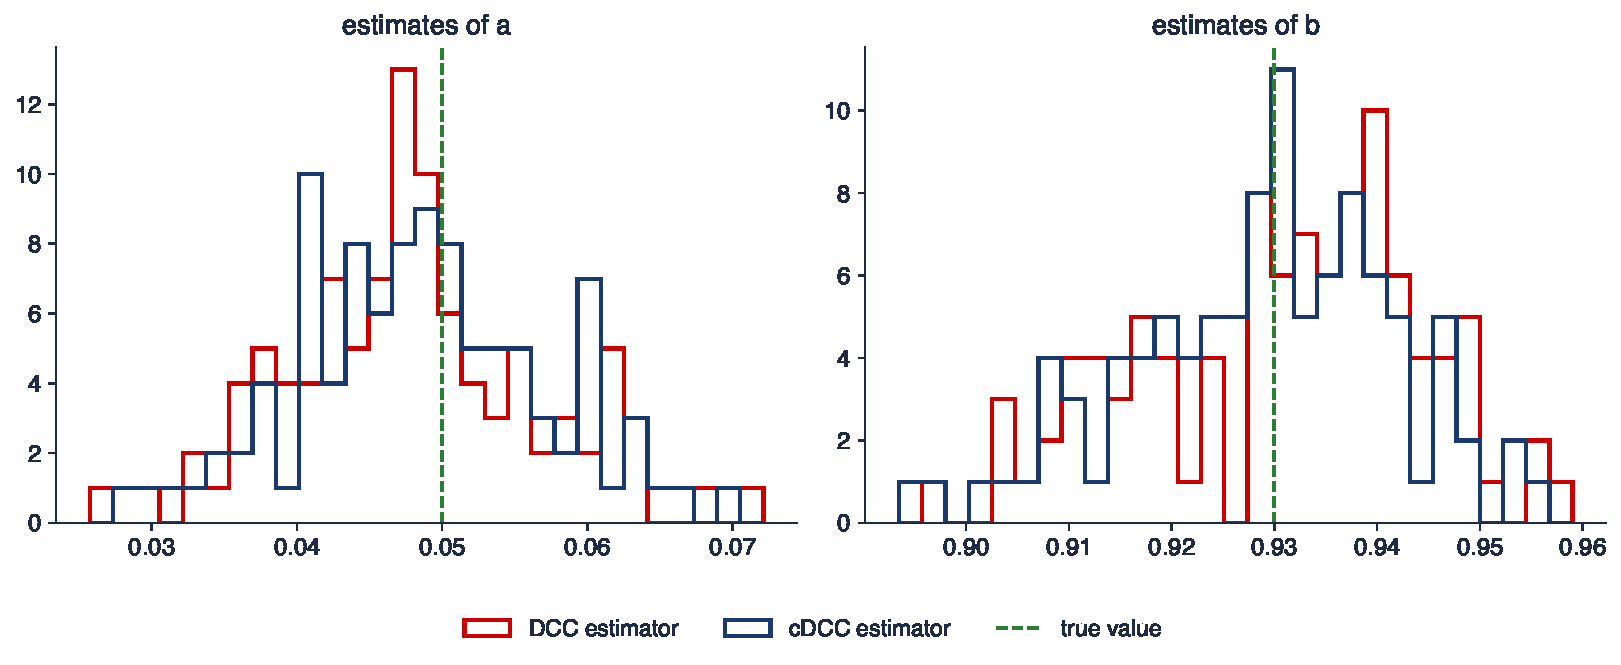
\includegraphics[width=0.97\textwidth,height=0.6\textheight,keepaspectratio]{ats_ch8_dcc_sim.pdf}
\end{center}
\vspace{-0.25cm}
\begin{itemize}
    \item Proces cDCC bivariat cu $a = 0{,}05$, $b = 0{,}93$, corelația-țintă 0,5, varianțe unitare; $T = 2\,000$, 100 de replicări; ambii estimatori pe fiecare eșantion
\end{itemize}
\quantlet{ATS\_ch8\_mgarch}{\qlurl{ATS_ch8_mgarch}}
\end{frame}

\begin{frame}{Interpretarea simulării DCC}
\itemsize{\small}
\begin{itemize}
    \item Estimațiile medii: DCC $\hat a = 0{,}0478$, $\hat b = 0{,}9307$; cDCC $\hat a = 0{,}0486$, $\hat b = 0{,}9288$ (valorile adevărate 0,05 și 0,93)
    \item RMSE pentru $\hat a$: 0{,}0090 (DCC) și 0{,}0086 (cDCC); pentru $\hat b$: 0{,}0135 și 0{,}0129: inconsistența este reală, dar mică la aceste niveluri de persistență
    \item Eroarea de eșantionare domină deplasarea la două mii de observații; diferența contează mai mult pentru țintă în sisteme mari și pentru inferența asupra lui $(a, b)$
    \item O demonstrație a inconsistenței nu spune cît de mare este deplasarea: simulați-o în propria configurație înainte de a alege estimatorul
\end{itemize}
\end{frame}

\begin{frame}{Matrice de covarianță mari: shrinkage și DCC-NL (1/2)}
\itemsize{\small}
\begin{itemize}
    \item Cînd $N/T$ nu este mic, valorile proprii ale unei covarianțe de eșantion $S$ sînt prea dispersate
    \begin{itemize}
        \item $N$: numărul de active; $T$: numărul de observații; cele mai mari valori proprii sînt prea mari, cele mai mici, prea mici; inversa $S^{-1}$ amplifică eroarea
    \end{itemize}
    \item Portofoliul de varianță minimă globală (GMV): ponderile cu cea mai mică varianță care însumează 1
    \[ w = \frac{\Sigma^{-1}\mathbf 1}{\mathbf 1'\Sigma^{-1}\mathbf 1} \]
    \begin{itemize}
        \item $\Sigma$: matricea de covarianță a randamentelor; $\mathbf 1$: vectorul cu toate elementele egale cu 1
        \item pune ponderi mari pe direcțiile cu valorile proprii cele mai mici, cel mai mult subestimate
        \item depinde doar de $\Sigma$, deci riscul lui realizat măsoară calitatea prognozei covarianței fără zgomotul randamentelor așteptate
    \end{itemize}
\end{itemize}
\end{frame}

\begin{frame}{Matrice de covarianță mari: shrinkage și DCC-NL (2/2)}
\itemsize{\small}
\begin{itemize}
    \item Shrinkage liniar \refLWa: o medie ponderată între $S$ și o matrice identitate scalată
    \[ \hat\Sigma = \delta\,\mu I + (1 - \delta)\,S \]
    \begin{itemize}
        \item $\mu$: media valorilor proprii ale lui $S$; $\delta \in [0, 1]$: intensitatea shrinkage-ului, estimată din date (mai mare cînd $N/T$ este mai mare)
    \end{itemize}
    \item Shrinkage neliniar \refLWb: se păstrează vectorii proprii ai lui $S$ și se înlocuiește fiecare valoare proprie $\lambda_i$ cu $d(\lambda_i)$
    \begin{itemize}
        \item $d(\cdot)$: o formulă analitică de tip kernel care ridică valorile proprii mici și le coboară pe cele mari, cu intensități diferite
    \end{itemize}
    \item DCC-NL \refELW: în DCC, ținta $S$ a reziduurilor standardizate este ea însăși o covarianță de eșantion mare: o înlocuim cu versiunea ei cu shrinkage neliniar
    \begin{itemize}
        \item verosimilitate compusă pentru $(a, b)$, GARCH univariat pentru varianțe; evaluat prin abaterea standard în afara eșantionului a portofoliilor GMV
    \end{itemize}
\end{itemize}
\end{frame}

\begin{frame}{Studiu de caz: Engle, Ledoit și Wolf (2019) pe acțiuni din SUA}
\itemsize{\footnotesize}
\begin{center}
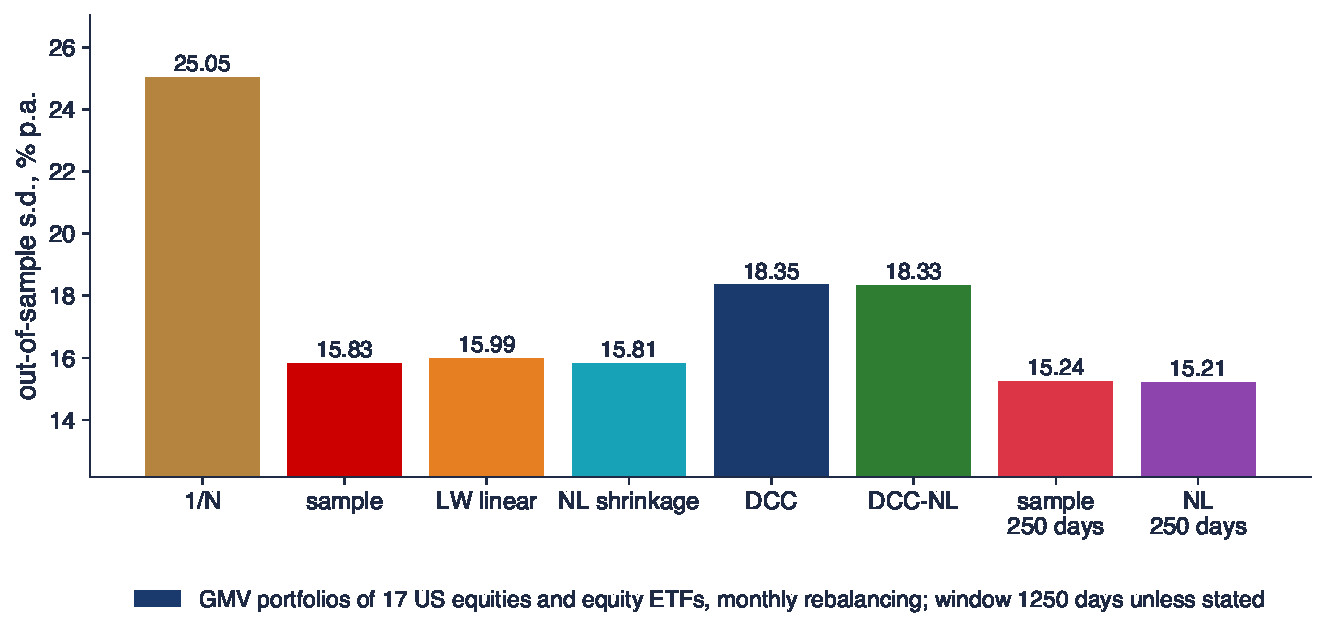
\includegraphics[width=0.97\textwidth,height=0.6\textheight,keepaspectratio]{ats_ch8_gmv.pdf}
\end{center}
\vspace{-0.25cm}
\begin{itemize}
    \item 17 active: 14 acțiuni din SUA și trei ETF-uri pe acțiuni (SPY, QQQ, RSP), care sînt ele însele portofolii de acțiuni; ponderi GMV rebalansate la fiecare 21 de zile din 23.05.2017 (112 rebalansări); fereastra de 1\,250 de zile, respectiv 250 de zile pentru ultimele două bare; abaterea standard anualizată în afara eșantionului
\end{itemize}
\quantlet{ATS\_ch8\_mgarch}{\qlurl{ATS_ch8_mgarch}}
\end{frame}

\begin{frame}{Interpretarea comparației GMV}
\itemsize{\small}
\begin{itemize}
    \item Abaterea standard în afara eșantionului (\% anual): 1/N 25{,}05, eșantion 15{,}83, shrinkage liniar 15{,}99, shrinkage neliniar 15{,}81, DCC 18{,}35, DCC-NL 18{,}33
    \item Cu $N/T = 17/1\,250$, covarianța de eșantion este deja precisă: shrinkage-ul neliniar schimbă puțin (15{,}81 față de 15{,}83); DCC-NL nu este mai bun decît DCC
    \item Aici dinamica dăunează: DCC (cu varianțe GARCH, prognoze mediate pe perioada de deținere de 21 de zile) dă 18{,}35 față de 15{,}83; prognozele de varianță pe o lună pentru acțiuni individuale precum MSTR și TSLA sînt zgomotoase, iar GMV le amplifică erorile
    \item Cu o fereastră de 250 de zile ($N/T$ de cinci ori mai mare), portofoliul GMV din eșantion are abaterea standard 15{,}24, iar cel cu shrinkage neliniar 15{,}21: doar cu 0{,}2\% mai mică, deși ETF-urile fac matricea de corelație aproape singulară (numărul de condiționare median 1146); fereastra mai scurtă reduce ea însăși riscul, o formă rudimentară de variație în timp
    \item Studiul original folosește sute de acțiuni, unde $N/T$ este mare și cîștigurile DCC-NL sînt substanțiale; cu $N$-ul nostru, lecția este cînd contează shrinkage-ul, nu cît cîștigă
\end{itemize}
\end{frame}

\begin{frame}{Covarianța realizată}
\itemsize{\small}
\begin{itemize}
    \item RV multivariat: suma produselor exterioare ale vectorilor de randamente intraday
    \[ \mathrm{RCov}_t = \sum_{i=1}^n r_{t,i}\,r_{t,i}' \to \int_0^1\Sigma_s\,ds \]
    \begin{itemize}
        \item $r_{t,i}$: vectorul $N \times 1$ al randamentelor intraday; $\Sigma_s$: matricea de covarianță instantanee; la limită se adaugă salturile comune; cu prețuri sincrone și fără zgomot, moștenește TLC a lui RV
    \end{itemize}
    \item Tranzacționarea asincronă: prețurile „previous-tick” creează randamente nule pentru activul care nu a fost tranzacționat; covarianțele se apropie de zero cînd intervalul scade (efectul Epps)
    \begin{itemize}
        \item eșantionarea la timpul de reîmprospătare (toate activele au fost tranzacționate) și realised kernel-ul multivariat \refBNHLSc: consistent și pozitiv semidefinit
    \end{itemize}
    \item Prognoza: HAR pe elementele factorului Cholesky al lui $\mathrm{RCov}_t$ păstrează prognozele pozitiv definite \refCV; HEAVY și Realized GARCH au versiuni multivariate
    \item Evaluarea prognozelor de covarianță $H_t$ față de un proxy matriceal $\Sigma_t$: funcții de pierdere robuste \refLRV
    \begin{itemize}
        \item QLIKE matriceal $\ln|H_t| + \mathrm{tr}(H_t^{-1}\Sigma_t)$, cu $|\cdot|$ determinantul și $\mathrm{tr}$ urma; MSE Frobenius, suma pătratelor erorilor pe elemente
    \end{itemize}
\end{itemize}
\end{frame}

\begin{frame}{Bitcoin și Ether: corelația realizată și corelația DCC}
\itemsize{\footnotesize}
\begin{center}
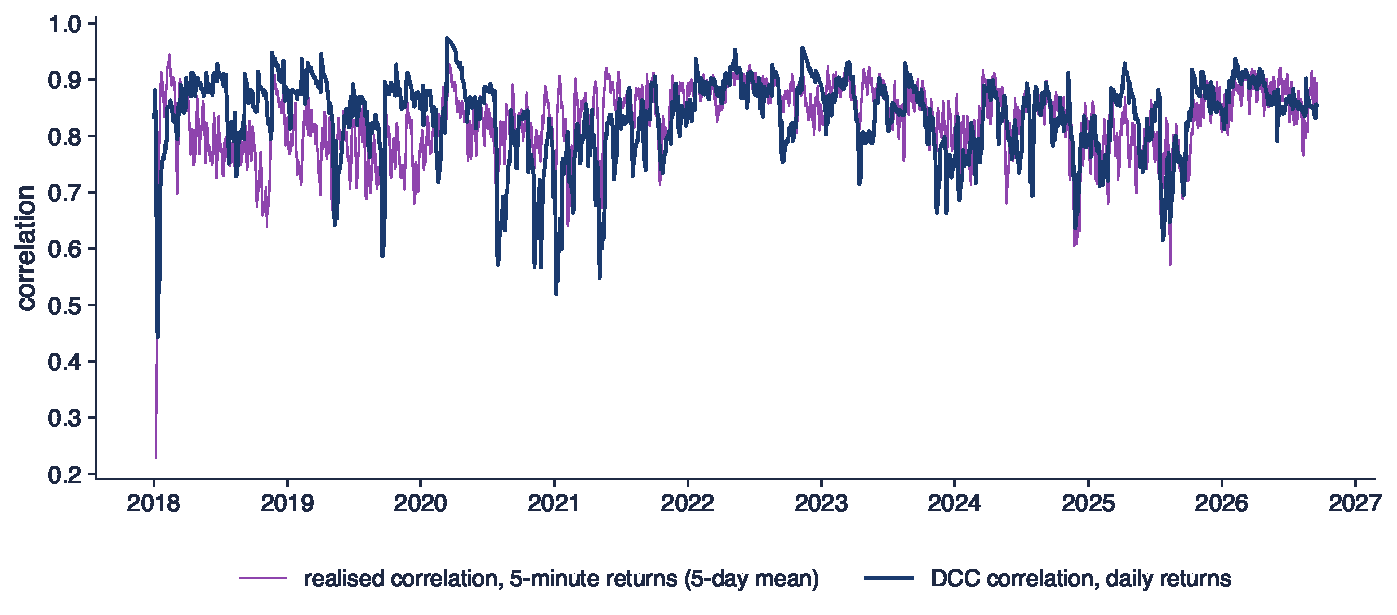
\includegraphics[width=0.97\textwidth,height=0.6\textheight,keepaspectratio]{ats_ch8_corr_crypto.pdf}
\end{center}
\vspace{-0.25cm}
\begin{itemize}
    \item Corelația realizată zilnică din randamente la 5 minute (medii pe 5 zile) și corelația DCC a randamentelor zilnice închidere--închidere (UTC), 2018--2026
\end{itemize}
\quantlet{ATS\_ch8\_mgarch}{\qlurl{ATS_ch8_mgarch}}
\end{frame}

\begin{frame}{Interpretarea corelațiilor}
\itemsize{\small}
\begin{itemize}
    \item Corelația realizată medie 0{,}83, corelația DCC medie 0{,}83; corelația dintre cele două serii 0{,}26
    \item DCC folosește o observație pe zi ($\hat a = 0{,}051$, $\hat b = 0{,}928$): netezește și reacționează cu întîrziere; măsura realizată se mișcă zilnic și scade repede în episoadele specifice unei monede (cuantila de 5\% 0{,}68)
    \item Combinarea lor (o măsură realizată în ecuația corelației) este analogul multivariat al Realized GARCH
    \item Eșantionarea la cinci minute se află pe partea plată a curbei Epps pentru aceste două monede (slide-ul cu signature plot): corelația realizată nu este deplasată spre zero
\end{itemize}
\end{frame}

\begin{frame}{Recapitulare: cazul multivariat}
\itemsize{\small}
\begin{itemize}
    \item BEKK garantează pozitivitatea cu un cost pătratic în parametri; DCC separă varianțele de corelații și funcționează pentru $N$ mare
    \item cDCC corectează inconsistența țintei DCC; în configurații moderate, diferența este mică
    \item În dimensiune mare, ținta are nevoie de shrinkage (DCC-NL); evaluați prin riscul GMV sau prin funcții de pierdere matriceale robuste
\end{itemize}
\end{frame}


%=============================================================================
\section{AI în descoperirea științifică}
%=============================================================================

\begin{frame}{O întrebare deschisă}
\itemsize{\small}
\begin{itemize}
    \item Îmbunătățește exploatarea erorii de măsurare a varianței realizate (HARQ) prognozele de volatilitate în mod robust sau doar pentru anumite alegeri de specificare?
    \begin{itemize}
        \item formal: raportul QLIKE HARQ/HAR și statistica DM pe o grilă preînregistrată (fereastră, filtru, măsură realizată, activ); infirmată dacă raportul depășește 1 sau testul DM este nesemnificativ în majoritatea celulelor
        \item măsura preciziei (RQ) este ea însăși zgomotoasă și cu cozi groase, deci cîștigul poate fi fragil
    \end{itemize}
    \item Miza: sistemele de risc folosesc zilnic prognoze de volatilitate pe o zi; un cîștig mic, dar robust valorează mai mult decît unul mare și fragil
    \begin{itemize}
        \item literatura de pornire: \refBPQ, \refCor, \refPat, \refHLb, \refHLN
    \end{itemize}
\end{itemize}
\end{frame}

\begin{frame}{Bucla de cercetare cu un asistent AI}
\itemsize{\footnotesize}
\begin{itemize}
    \item Un asistent AI (un LLM precum Claude, ChatGPT, Gemini sau Copilot) accelerează fiecare etapă; Semantic Scholar și Elicit ajută la literatură
    \begin{itemize}
        \item \textbf{literatura}: \aiprompt{Listează lucrări recenzate din 2016 încoace care testează în afara eșantionului modele de tip HARQ pe alte active decît acțiunile din SUA; dă DOI-urile.} Apoi verificați fiecare DOI pe Crossref
        \item \textbf{ipoteza}: \aiprompt{În ce condiții ale datelor (tranzacționare 24/7, salturi, randamente nule) ar trebui să scadă sau să crească cîștigul HARQ? Dă predicții testabile.}
        \item \textbf{cod și replicare}: cereți prognoze HAR și HARQ pe fereastră mobilă, apoi reproduceți întîi o cifră cunoscută (raportul QLIKE pentru Bitcoin din acest curs)
        \item \textbf{robustețe și critică}: \aiprompt{Joacă rolul unui recenzent ostil: ce alegeri dintr-o comparație a prognozelor HARQ ar putea produce un cîștig fals?}
    \end{itemize}
    \item Raportul: ce s-a cerut, ce s-a păstrat, ce s-a respins (AI\_USE.md, AI\_ERRORS.md)
\end{itemize}
\end{frame}

\begin{frame}{Verificări necesare}
\itemsize{\small}
\begin{itemize}
    \item Fiecare referință există și spune ce se afirmă (DOI-ul funcționează, titlul coincide, rezultatul se află în lucrare)
    \item Prognoza din $t$ folosește doar date pînă la $t$: ferestrele, centrarea lui RQ, filtrul de plauzibilitate și corecția deplasării prognozelor în logaritmi sînt calculate în fereastra de estimare
    \item Funcția de pierdere este robustă (QLIKE, MSE), iar proxy-ul este precizat; statisticile DM folosesc varianțe HAC
    \item Toate celulele grilei sînt raportate, nu doar cea mai bună; numărul comparațiilor este precizat
    \item Măsurile realizate sînt recalculate din prețurile brute și concordă cu o sursă independentă pentru activele și datele comune
\end{itemize}
\end{frame}

\begin{frame}{Mini studiu de caz: douăsprezece alegeri, o singură concluzie?}
\itemsize{\footnotesize}
\begin{center}
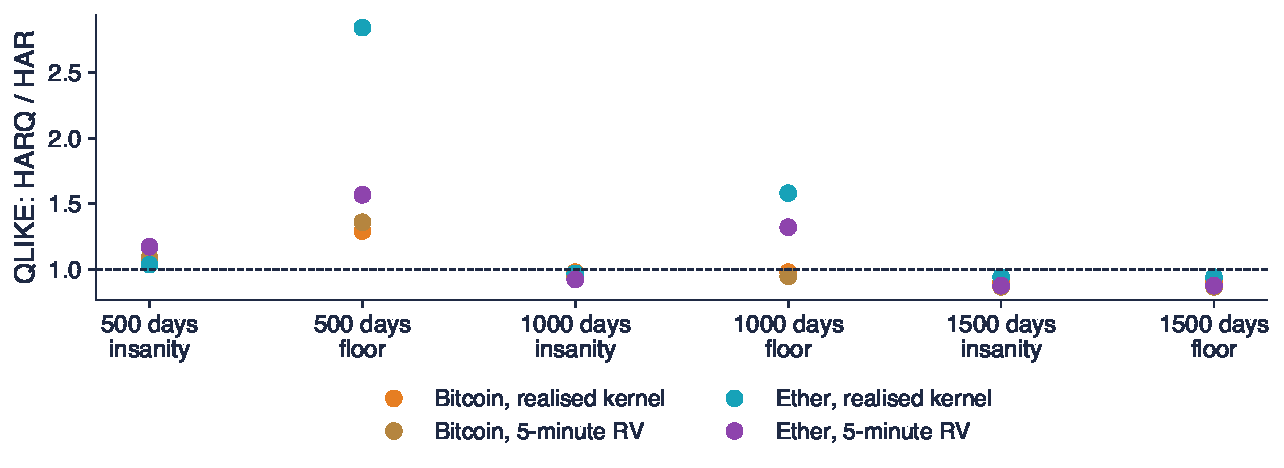
\includegraphics[width=0.97\textwidth,height=0.6\textheight,keepaspectratio]{ats_ch8_ai_case.pdf}
\end{center}
\vspace{-0.25cm}
\begin{itemize}
    \item Raportul QLIKE HARQ/HAR pentru Bitcoin și Ether: fereastră de 500, 1\,000 sau 1\,500 de zile; filtrul de plauzibilitate sau o limită inferioară egală cu cel mai mic RV din eșantion; ținta RV la 5 minute sau realised kernel
    \item Rapoarte între 0{,}865 și 2{,}844; HARQ mai bun în 58\% dintre cele 24 de celule, semnificativ mai bun (DM $< -1{,}96$) în 50\%, semnificativ mai slab în 12\%: un rezumat AI care raportează o singură celulă ar ascunde cea mai mare parte din acest tablou
\end{itemize}
\quantlet{ATS\_ch8\_ai\_robustness}{\qlurl{ATS_ch8_ai_robustness}}
\end{frame}

\begin{frame}{Idee de proiect}
\itemsize{\small}
\begin{itemize}
    \item \textbf{Volatilitatea realizată a criptoactivelor: se transferă instrumentele de la acțiuni?}: întîi replicare, apoi extindere
    \begin{itemize}
        \item replicați: HAR și HARQ din acest curs pentru Bitcoin (raportul QLIKE 0{,}946) și Realized GARCH pentru S\&P 500 (persistența 0{,}968)
        \item extindeți: zece monede din arhiva Binance; măsuri robuste la zgomot din date la o secundă; o corecție a sezonalității intraday înaintea testelor de salt; Realized GARCH cu realised kernel; data ETF-urilor spot (ianuarie 2024) ca ruptură naturală
        \item preînregistrați: activele, eșantionul, măsurile, modelele, ferestrele, funcțiile de pierdere, testele DM/MCS și grila de robustețe
    \end{itemize}
    \item Livrabilele urmează regulile cursului: repository, raport, AI\_USE.md, AI\_ERRORS.md, susținere orală
\end{itemize}
\end{frame}


%=============================================================================
\section{Încheiere}
%=============================================================================

\begin{frame}{Idei de reținut}
\itemsize{\small}
\begin{itemize}
    \item QML gaussian are nevoie doar de ecuația varianței; cu cozi groase, folosiți erorile standard sandwich
    \item Volatilitatea are componente rapide și lente; factorii macroeconomici ai celei lente au nevoie de eșantioane lungi și de rapoarte de varianță raportate fără selecție
    \item Măsurile realizate fac volatilitatea observabilă, cu o eroare cunoscută; zgomotul și salturile decid estimatorul
    \item La un pas, HAR, HARQ și Realized GARCH depășesc modelele care folosesc doar randamentele; evaluați cu QLIKE sau MSE
    \item În multe dimensiuni, ținta de corelație are nevoie de shrinkage (DCC-NL); dacă dinamica ajută trebuie verificat în afara eșantionului
\end{itemize}
\end{frame}

\begin{frame}{Autoevaluare}
\itemsize{\small}
\begin{columns}[T]
\begin{column}{0.58\textwidth}
\begin{block}{Întrebări}
\begin{itemize}
    \item De ce sînt prea mici erorile standard din hessiană pentru GARCH cînd $\kappa_\eta > 3$?
    \item Ce măsoară raportul de varianță din GARCH-MIDAS?
    \item De ce contează convergența stabilă pentru TLC a lui RV?
    \item De ce poate crește un signature plot la frecvență înaltă?
    \item De ce ne așteptăm ca $\beta_{dQ}$ să fie negativ în HARQ?
    \item Ce funcții de pierdere păstrează ordinea cu un proxy zgomotos?
\end{itemize}
\end{block}
\end{column}
\begin{column}{0.38\textwidth}
\begin{block}{Urmează: \atschlink{https://danpele.github.io/Advanced-Time-Series/RO/Cursuri/capitol9_var_es_backtesting.pdf}{Capitolul 9}}
\begin{itemize}
    \item VaR, ES și backtesting: elicitabilitate, funcții de scor și riscul de model
    \item De la prognozele de volatilitate la prognozele de coadă: VaR 1\% și ES 2,5\%, funcțiile lor de scor și backtesting-ul
\end{itemize}
\end{block}
\end{column}
\end{columns}
\end{frame}


%=============================================================================
\section{Anexă}
%=============================================================================

\begin{frame}{Anexă: sandwich-ul GARCH}
\hypertarget{atsapp1}{}\atsappback{atssrc1}{Înapoi}
\itemsize{\small}
\begin{itemize}
    \item $\ell_t = -\frac12(\ln\sigma^2_t + \varepsilon^2_t/\sigma^2_t)$, $d_t = \sigma_t^{-2}\partial\sigma^2_t/\partial\theta$: $s_t = \frac12(\eta^2_t - 1)d_t$ în $\theta_0$
    \item $B = \E s_ts_t' = \frac14\E(\eta^2_t - 1)^2\,\E d_td_t' = \frac{\kappa_\eta - 1}{4}J$, deoarece $\eta_t$ este independent de $d_t \in \mathcal F_{t-1}$
    \item $\partial s_t/\partial\theta' = -\frac12\eta^2_td_td_t' + \frac12(\eta^2_t - 1)\partial d_t/\partial\theta'$; al doilea termen are media zero, deci $A = \frac12J$
    \item $A^{-1}B\,A^{-1} = 4J^{-1}\cdot\frac{\kappa_\eta - 1}{4}J\cdot J^{-1} = (\kappa_\eta - 1)J^{-1}$; doar hessiana: $A^{-1} = 2J^{-1}$; OPG: $B^{-1} = \frac{4}{\kappa_\eta - 1}J^{-1}$
\end{itemize}
\end{frame}

\begin{frame}{Anexă: deplasarea din zgomot a varianței realizate}
\hypertarget{atsapp2}{}\atsappback{atssrc2}{Înapoi}
\itemsize{\small}
\begin{itemize}
    \item $\tilde r_i = Y_{i/n} - Y_{(i-1)/n} = r_i + u_i - u_{i-1}$, cu $u$ i.i.d. $(0, \omega^2)$, independent de $X$
    \item $\sum_i\tilde r_i^2 = \sum_ir_i^2 + 2\sum_ir_i(u_i - u_{i-1}) + \sum_i(u_i - u_{i-1})^2$; termenul mixt are media zero, ultimul are media $2n\omega^2$
    \item $\Cov(\tilde r_i, \tilde r_{i-1}) = -\omega^2$: autocorelație negativă de ordinul întîi; realised kernel-ul adaugă $2\gamma_1 \approx -2n\omega^2$ și elimină deplasarea
    \item Randamentele autocorelate pozitiv (ajustarea treptată a prețului, prețuri stale (neactualizate)) dau $\gamma_1 > 0$ și un signature plot care crește cu intervalul; kernel-ul corectează ambele semne
\end{itemize}
\end{frame}

\begin{frame}{Anexă: atenuarea și HARQ}
\hypertarget{atsapp3}{}\atsappback{atssrc3}{Înapoi}
\itemsize{\small}
\begin{itemize}
    \item $\mathrm{IV}_{t+1} = c + \phi\,\mathrm{IV}_t + v_{t+1}$, observăm $\mathrm{RV}_t = \mathrm{IV}_t + e_t$, $e_t$ necorelat cu $\mathrm{IV}_t$ și $v_{t+1}$
    \item OLS pentru $\mathrm{RV}_{t+1}$ pe $\mathrm{RV}_t$: $\mathrm{plim}\,\hat\phi = \frac{\Cov(\mathrm{IV}_{t+1}, \mathrm{IV}_t)}{\Var(\mathrm{IV}_t) + \Var(e_t)} = \phi\lambda$, $\lambda = \frac{\Var(\mathrm{IV})}{\Var(\mathrm{IV}) + \E\Var(e_t)}$
    \item Cel mai bun predictor liniar, dată precizia de azi, folosește $\phi\lambda_t$, $\lambda_t = \frac{\Var(\mathrm{IV})}{\Var(\mathrm{IV}) + 2\mathrm{IQ}_t/n}$: descrescător în $\mathrm{IQ}_t$
    \item O dezvoltare de ordinul întîi în $\sqrt{\mathrm{IQ}_t}$ dă $\beta_d + \beta_{dQ}\sqrt{\mathrm{RQ}_t}$, cu $\beta_{dQ} < 0$: specificarea HARQ \refBPQ
\end{itemize}
\end{frame}


%=============================================================================
\section{Bibliografie}
%=============================================================================

\begin{frame}{Bibliografie (1/5)}
\itemsize{\tiny}
\begin{itemize}
    \item Aielli, G. P. (2013). Dynamic conditional correlation: On properties and estimation. \textit{Journal of Business \& Economic Statistics}, 31(3), 282--299. \href{https://doi.org/10.1080/07350015.2013.771027}{doi:10.1080/07350015.2013.771027}
    \item Andersen, T. G., \& Bollerslev, T. (1998). Answering the skeptics: Yes, standard volatility models do provide accurate forecasts. \textit{International Economic Review}, 39(4), 885--905. \href{https://doi.org/10.2307/2527343}{doi:10.2307/2527343}
    \item Andersen, T. G., Bollerslev, T., \& Diebold, F. X. (2007). Roughing it up: Including jump components in the measurement, modeling, and forecasting of return volatility. \textit{The Review of Economics and Statistics}, 89(4), 701--720. \href{https://doi.org/10.1162/rest.89.4.701}{doi:10.1162/rest.89.4.701}
    \item Andersen, T. G., Bollerslev, T., Diebold, F. X., \& Labys, P. (2003). Modeling and forecasting realized volatility. \textit{Econometrica}, 71(2), 579--625. \href{https://doi.org/10.1111/1468-0262.00418}{doi:10.1111/1468-0262.00418}
    \item Andersen, T. G., Dobrev, D., \& Schaumburg, E. (2012). Jump-robust volatility estimation using nearest neighbor truncation. \textit{Journal of Econometrics}, 169(1), 75--93. \href{https://doi.org/10.1016/j.jeconom.2012.01.011}{doi:10.1016/j.jeconom.2012.01.011}
    \item Bandi, F. M., \& Russell, J. R. (2008). Microstructure noise, realized variance, and optimal sampling. \textit{The Review of Economic Studies}, 75(2), 339--369. \href{https://doi.org/10.1111/j.1467-937X.2008.00474.x}{doi:10.1111/j.1467-937X.2008.00474.x}
    \item Barndorff-Nielsen, O. E., Hansen, P. R., Lunde, A., \& Shephard, N. (2008). Designing realized kernels to measure the ex post variation of equity prices in the presence of noise. \textit{Econometrica}, 76(6), 1481--1536. \href{https://doi.org/10.3982/ECTA6495}{doi:10.3982/ECTA6495}
    \item Barndorff-Nielsen, O. E., Hansen, P. R., Lunde, A., \& Shephard, N. (2009). Realized kernels in practice: Trades and quotes. \textit{The Econometrics Journal}, 12(3), C1--C32. \href{https://doi.org/10.1111/j.1368-423X.2008.00275.x}{doi:10.1111/j.1368-423X.2008.00275.x}
    \item Barndorff-Nielsen, O. E., Hansen, P. R., Lunde, A., \& Shephard, N. (2011). Multivariate realised kernels: Consistent positive semi-definite estimators of the covariation of equity prices with noise and non-synchronous trading. \textit{Journal of Econometrics}, 162(2), 149--169. \href{https://doi.org/10.1016/j.jeconom.2010.07.009}{doi:10.1016/j.jeconom.2010.07.009}
    \item Barndorff-Nielsen, O. E., \& Shephard, N. (2002). Econometric analysis of realized volatility and its use in estimating stochastic volatility models. \textit{Journal of the Royal Statistical Society: Series B}, 64(2), 253--280. \href{https://doi.org/10.1111/1467-9868.00336}{doi:10.1111/1467-9868.00336}
    \item Barndorff-Nielsen, O. E., \& Shephard, N. (2004). Power and bipower variation with stochastic volatility and jumps. \textit{Journal of Financial Econometrics}, 2(1), 1--37. \href{https://doi.org/10.1093/jjfinec/nbh001}{doi:10.1093/jjfinec/nbh001}
    \item Barndorff-Nielsen, O. E., \& Shephard, N. (2006). Econometrics of testing for jumps in financial economics using bipower variation. \textit{Journal of Financial Econometrics}, 4(1), 1--30. \href{https://doi.org/10.1093/jjfinec/nbi022}{doi:10.1093/jjfinec/nbi022}
\end{itemize}
\end{frame}

\begin{frame}{Bibliografie (2/5)}
\itemsize{\tiny}
\begin{itemize}
    \item Berkes, I., Horváth, L., \& Kokoszka, P. (2003). GARCH processes: Structure and estimation. \textit{Bernoulli}, 9(2), 201--227. \href{https://doi.org/10.3150/bj/1068128975}{doi:10.3150/bj/1068128975}
    \item Bollerslev, T. (1986). Generalized autoregressive conditional heteroskedasticity. \textit{Journal of Econometrics}, 31(3), 307--327. \href{https://doi.org/10.1016/0304-4076(86)90063-1}{doi:10.1016/0304-4076(86)90063-1}
    \item Bollerslev, T. (1990). Modelling the coherence in short-run nominal exchange rates: A multivariate generalized ARCH model. \textit{The Review of Economics and Statistics}, 72(3), 498--505. \href{https://doi.org/10.2307/2109358}{doi:10.2307/2109358}
    \item Bollerslev, T., Patton, A. J., \& Quaedvlieg, R. (2016). Exploiting the errors: A simple approach for improved volatility forecasting. \textit{Journal of Econometrics}, 192(1), 1--18. \href{https://doi.org/10.1016/j.jeconom.2015.10.007}{doi:10.1016/j.jeconom.2015.10.007}
    \item Bollerslev, T., \& Wooldridge, J. M. (1992). Quasi-maximum likelihood estimation and inference in dynamic models with time-varying covariances. \textit{Econometric Reviews}, 11(2), 143--172. \href{https://doi.org/10.1080/07474939208800229}{doi:10.1080/07474939208800229}
    \item Chiriac, R., \& Voev, V. (2011). Modelling and forecasting multivariate realized volatility. \textit{Journal of Applied Econometrics}, 26(6), 922--947. \href{https://doi.org/10.1002/jae.1152}{doi:10.1002/jae.1152}
    \item Comte, F., \& Lieberman, O. (2003). Asymptotic theory for multivariate GARCH processes. \textit{Journal of Multivariate Analysis}, 84(1), 61--84. \href{https://doi.org/10.1016/S0047-259X(02)00009-X}{doi:10.1016/S0047-259X(02)00009-X}
    \item Conrad, C., \& Kleen, O. (2020). Two are better than one: Volatility forecasting using multiplicative component GARCH-MIDAS models. \textit{Journal of Applied Econometrics}, 35(1), 19--45. \href{https://doi.org/10.1002/jae.2742}{doi:10.1002/jae.2742}
    \item Corsi, F. (2009). A simple approximate long-memory model of realized volatility. \textit{Journal of Financial Econometrics}, 7(2), 174--196. \href{https://doi.org/10.1093/jjfinec/nbp001}{doi:10.1093/jjfinec/nbp001}
    \item Diebold, F. X., \& Mariano, R. S. (1995). Comparing predictive accuracy. \textit{Journal of Business \& Economic Statistics}, 13(3), 253--263. \href{https://doi.org/10.1080/07350015.1995.10524599}{doi:10.1080/07350015.1995.10524599}
    \item Engle, R. (2002). Dynamic conditional correlation: A simple class of multivariate generalized autoregressive conditional heteroskedasticity models. \textit{Journal of Business \& Economic Statistics}, 20(3), 339--350. \href{https://doi.org/10.1198/073500102288618487}{doi:10.1198/073500102288618487}
    \item Engle, R. F. (1982). Autoregressive conditional heteroscedasticity with estimates of the variance of United Kingdom inflation. \textit{Econometrica}, 50(4), 987--1007. \href{https://doi.org/10.2307/1912773}{doi:10.2307/1912773}
\end{itemize}
\end{frame}

\begin{frame}{Bibliografie (3/5)}
\itemsize{\tiny}
\begin{itemize}
    \item Engle, R. F., Ghysels, E., \& Sohn, B. (2013). Stock market volatility and macroeconomic fundamentals. \textit{The Review of Economics and Statistics}, 95(3), 776--797. \href{https://doi.org/10.1162/REST_a_00300}{doi:10.1162/REST\_a\_00300}
    \item Engle, R. F., \& Kroner, K. F. (1995). Multivariate simultaneous generalized ARCH. \textit{Econometric Theory}, 11(1), 122--150. \href{https://doi.org/10.1017/S0266466600009063}{doi:10.1017/S0266466600009063}
    \item Engle, R. F., Ledoit, O., \& Wolf, M. (2019). Large dynamic covariance matrices. \textit{Journal of Business \& Economic Statistics}, 37(2), 363--375. \href{https://doi.org/10.1080/07350015.2017.1345683}{doi:10.1080/07350015.2017.1345683}
    \item Engle, R. F., \& Lee, G. G. J. (1999). A long-run and short-run component model of stock return volatility. In R. F. Engle \& H. White (Eds.), \textit{Cointegration, Causality, and Forecasting: A Festschrift in Honour of Clive W. J. Granger} (pp.\ 475--497). Oxford University Press. \href{https://doi.org/10.1093/oso/9780198296836.003.0020}{doi:10.1093/oso/9780198296836.003.0020}
    \item Engle, R. F., \& Sheppard, K. (2001). Theoretical and empirical properties of dynamic conditional correlation multivariate GARCH. \textit{NBER Working Paper} 8554. \href{https://doi.org/10.3386/w8554}{doi:10.3386/w8554}
    \item Epps, T. W. (1979). Comovements in stock prices in the very short run. \textit{Journal of the American Statistical Association}, 74(366), 291--298. \href{https://doi.org/10.1080/01621459.1979.10482508}{doi:10.1080/01621459.1979.10482508}
    \item Francq, C., \& Zakoïan, J.-M. (2004). Maximum likelihood estimation of pure GARCH and ARMA-GARCH processes. \textit{Bernoulli}, 10(4), 605--637. \href{https://doi.org/10.3150/bj/1093265632}{doi:10.3150/bj/1093265632}
    \item Francq, C., \& Zakoïan, J.-M. (2019). \textit{GARCH Models: Structure, Statistical Inference and Financial Applications} (2nd ed.). Wiley. \href{https://doi.org/10.1002/9781119313472}{doi:10.1002/9781119313472}
    \item Ghysels, E., Santa-Clara, P., \& Valkanov, R. (2006). Predicting volatility: Getting the most out of return data sampled at different frequencies. \textit{Journal of Econometrics}, 131(1--2), 59--95. \href{https://doi.org/10.1016/j.jeconom.2005.01.004}{doi:10.1016/j.jeconom.2005.01.004}
    \item Glosten, L. R., Jagannathan, R., \& Runkle, D. E. (1993). On the relation between the expected value and the volatility of the nominal excess return on stocks. \textit{The Journal of Finance}, 48(5), 1779--1801. \href{https://doi.org/10.1111/j.1540-6261.1993.tb05128.x}{doi:10.1111/j.1540-6261.1993.tb05128.x}
    \item Hafner, C. M., \& Preminger, A. (2009). On asymptotic theory for multivariate GARCH models. \textit{Journal of Multivariate Analysis}, 100(9), 2044--2054. \href{https://doi.org/10.1016/j.jmva.2009.03.011}{doi:10.1016/j.jmva.2009.03.011}
    \item Hamilton, J. D. (1994). \textit{Time Series Analysis}. Princeton University Press. \href{https://doi.org/10.2307/j.ctv14jx6sm}{doi:10.2307/j.ctv14jx6sm}
\end{itemize}
\end{frame}

\begin{frame}{Bibliografie (4/5)}
\itemsize{\tiny}
\begin{itemize}
    \item Hansen, P. R., \& Huang, Z. (2016). Exponential GARCH modeling with realized measures of volatility. \textit{Journal of Business \& Economic Statistics}, 34(2), 269--287. \href{https://doi.org/10.1080/07350015.2015.1038543}{doi:10.1080/07350015.2015.1038543}
    \item Hansen, P. R., Huang, Z., \& Shek, H. H. (2012). Realized GARCH: A joint model for returns and realized measures of volatility. \textit{Journal of Applied Econometrics}, 27(6), 877--906. \href{https://doi.org/10.1002/jae.1234}{doi:10.1002/jae.1234}
    \item Hansen, P. R., \& Lunde, A. (2005). A forecast comparison of volatility models: Does anything beat a GARCH(1,1)? \textit{Journal of Applied Econometrics}, 20(7), 873--889. \href{https://doi.org/10.1002/jae.800}{doi:10.1002/jae.800}
    \item Hansen, P. R., \& Lunde, A. (2006a). Consistent ranking of volatility models. \textit{Journal of Econometrics}, 131(1--2), 97--121. \href{https://doi.org/10.1016/j.jeconom.2005.01.005}{doi:10.1016/j.jeconom.2005.01.005}
    \item Hansen, P. R., \& Lunde, A. (2006b). Realized variance and market microstructure noise. \textit{Journal of Business \& Economic Statistics}, 24(2), 127--161. \href{https://doi.org/10.1198/073500106000000071}{doi:10.1198/073500106000000071}
    \item Hansen, P. R., Lunde, A., \& Nason, J. M. (2011). The model confidence set. \textit{Econometrica}, 79(2), 453--497. \href{https://doi.org/10.3982/ECTA5771}{doi:10.3982/ECTA5771}
    \item Heber, G., Lunde, A., Shephard, N., \& Sheppard, K. (2009). \textit{Oxford-Man Institute's realized library}, version 0.3. Oxford-Man Institute, University of Oxford (discontinued in 2022; copy of 28 February 2022 preserved by the Internet Archive). \href{https://web.archive.org/web/2021/https://realized.oxford-man.ox.ac.uk/terms-and-conditions}{web.archive.org}
    \item Huang, X., \& Tauchen, G. (2005). The relative contribution of jumps to total price variance. \textit{Journal of Financial Econometrics}, 3(4), 456--499. \href{https://doi.org/10.1093/jjfinec/nbi025}{doi:10.1093/jjfinec/nbi025}
    \item Jacod, J., Li, Y., Mykland, P. A., Podolskij, M., \& Vetter, M. (2009). Microstructure noise in the continuous case: The pre-averaging approach. \textit{Stochastic Processes and their Applications}, 119(7), 2249--2276. \href{https://doi.org/10.1016/j.spa.2008.11.004}{doi:10.1016/j.spa.2008.11.004}
    \item Jensen, S. T., \& Rahbek, A. (2004). Asymptotic inference for nonstationary GARCH. \textit{Econometric Theory}, 20(6), 1203--1226. \href{https://doi.org/10.1017/S0266466604206065}{doi:10.1017/S0266466604206065}
    \item Laurent, S., Rombouts, J. V. K., \& Violante, F. (2012). On the forecasting accuracy of multivariate GARCH models. \textit{Journal of Applied Econometrics}, 27(6), 934--955. \href{https://doi.org/10.1002/jae.1248}{doi:10.1002/jae.1248}
    \item Ledoit, O., \& Wolf, M. (2004). A well-conditioned estimator for large-dimensional covariance matrices. \textit{Journal of Multivariate Analysis}, 88(2), 365--411. \href{https://doi.org/10.1016/S0047-259X(03)00096-4}{doi:10.1016/S0047-259X(03)00096-4}
\end{itemize}
\end{frame}

\begin{frame}{Bibliografie (5/5)}
\itemsize{\tiny}
\begin{itemize}
    \item Ledoit, O., \& Wolf, M. (2020). Analytical nonlinear shrinkage of large-dimensional covariance matrices. \textit{The Annals of Statistics}, 48(5), 3043--3065. \href{https://doi.org/10.1214/19-AOS1921}{doi:10.1214/19-AOS1921}
    \item Lee, S. S., \& Mykland, P. A. (2008). Jumps in financial markets: A new nonparametric test and jump dynamics. \textit{The Review of Financial Studies}, 21(6), 2535--2563. \href{https://doi.org/10.1093/rfs/hhm056}{doi:10.1093/rfs/hhm056}
    \item Lee, S.-W., \& Hansen, B. E. (1994). Asymptotic theory for the GARCH(1,1) quasi-maximum likelihood estimator. \textit{Econometric Theory}, 10(1), 29--52. \href{https://doi.org/10.1017/S0266466600008215}{doi:10.1017/S0266466600008215}
    \item Ling, S., \& McAleer, M. (2003). Asymptotic theory for a vector ARMA-GARCH model. \textit{Econometric Theory}, 19(2), 280--310. \href{https://doi.org/10.1017/S0266466603192092}{doi:10.1017/S0266466603192092}
    \item Lumsdaine, R. L. (1996). Consistency and asymptotic normality of the quasi-maximum likelihood estimator in IGARCH(1,1) and covariance stationary GARCH(1,1) models. \textit{Econometrica}, 64(3), 575--596. \href{https://doi.org/10.2307/2171862}{doi:10.2307/2171862}
    \item Newey, W. K., \& West, K. D. (1987). A simple, positive semi-definite, heteroskedasticity and autocorrelation consistent covariance matrix. \textit{Econometrica}, 55(3), 703--708. \href{https://doi.org/10.2307/1913610}{doi:10.2307/1913610}
    \item Pakel, C., Shephard, N., Sheppard, K., \& Engle, R. F. (2021). Fitting vast dimensional time-varying covariance models. \textit{Journal of Business \& Economic Statistics}, 39(3), 652--668. \href{https://doi.org/10.1080/07350015.2020.1713795}{doi:10.1080/07350015.2020.1713795}
    \item Patton, A. J. (2011). Volatility forecast comparison using imperfect volatility proxies. \textit{Journal of Econometrics}, 160(1), 246--256. \href{https://doi.org/10.1016/j.jeconom.2010.03.034}{doi:10.1016/j.jeconom.2010.03.034}
    \item Patton, A. J., \& Sheppard, K. (2015). Good volatility, bad volatility: Signed jumps and the persistence of volatility. \textit{The Review of Economics and Statistics}, 97(3), 683--697. \href{https://doi.org/10.1162/REST_a_00503}{doi:10.1162/REST\_a\_00503}
    \item Petropoulos, F., Apiletti, D., Assimakopoulos, V., Babai, M. Z., et al.\ (2022). Forecasting: Theory and practice. \textit{International Journal of Forecasting}, 38(3), 705--871. \href{https://doi.org/10.1016/j.ijforecast.2021.11.001}{doi:10.1016/j.ijforecast.2021.11.001}
    \item Shephard, N., \& Sheppard, K. (2010). Realising the future: Forecasting with high-frequency-based volatility (HEAVY) models. \textit{Journal of Applied Econometrics}, 25(2), 197--231. \href{https://doi.org/10.1002/jae.1158}{doi:10.1002/jae.1158}
    \item Zhang, L., Mykland, P. A., \& Aït-Sahalia, Y. (2005). A tale of two time scales: Determining integrated volatility with noisy high-frequency data. \textit{Journal of the American Statistical Association}, 100(472), 1394--1411. \href{https://doi.org/10.1198/016214505000000169}{doi:10.1198/016214505000000169}
\end{itemize}
\end{frame}

\end{document}
